\documentclass{article}

\usepackage[colorlinks, urlcolor=blue, linkcolor=red, citecolor=green]{hyperref}
\usepackage{fancyhdr} %设置页眉和页脚的
\usepackage{extramarks} %设置continue那玩意的
\usepackage{amsmath}
\usepackage{amsthm}
\usepackage{amsfonts}
\usepackage{tikz} %画线的
\usepackage[plain]{algorithm}
\usepackage{algpseudocode}
\usepackage{enumerate}

\usetikzlibrary{automata,positioning}

%表
\usepackage{booktabs}
\usepackage{multirow}
\usepackage{array}
\usepackage{caption}
\DeclareCaptionFont{heiti}{\heiti} %还可以定义其他的
\captionsetup{labelsep=space, font={small, bf}, skip=2pt} %space可以改成quad

%图
%*****************图片及其相关设置***************************
\usepackage{graphicx}
\graphicspath{{tupian/}}
\usepackage{subfigure}
%

%*****************代码相关设置***************************
\usepackage{pythonhighlight}

\usepackage{dsfont}
% Basic Document Settings
%

\topmargin=-0.45in
\evensidemargin=0in
\oddsidemargin=0in
\textwidth=6.5in
\textheight=9.0in
\headsep=0.25in

\linespread{1.1}

\pagestyle{fancy}
\lhead{\hmwkAuthorName}
\chead{\hmwkClass: \hmwkTitle}
\rhead{\firstxmark}
\lfoot{\lastxmark}
\cfoot{\thepage}

\renewcommand\headrulewidth{0.4pt}
\renewcommand\footrulewidth{0.4pt}

\setlength\parindent{0pt}

%
% Create Problem Sections
%

\newcommand{\enterProblemHeader}[1]{
    \nobreak\extramarks{}{Assignment A4.\arabic{#1} continued on next page\ldots}\nobreak{}
    \nobreak\extramarks{Assignment A4.\arabic{#1} (continued)}{Assignment A4.\arabic{#1} continued on next page\ldots}\nobreak{}
}

\newcommand{\exitProblemHeader}[1]{
    \nobreak\extramarks{Assignment A4.\arabic{#1} (continued)}{Assignment A4.\arabic{#1} continued on next page\ldots}\nobreak{}
    \stepcounter{#1}
    \nobreak\extramarks{Assignment A4.\arabic{#1}}{}\nobreak{}
}

\setcounter{secnumdepth}{0}
\newcounter{partCounter}
\newcounter{homeworkProblemCounter}
\setcounter{homeworkProblemCounter}{1}
\nobreak\extramarks{Assignment A4.\arabic{homeworkProblemCounter}}{}\nobreak{}

\newenvironment{homeworkProblem}{
    \section{Assignment A4.\arabic{homeworkProblemCounter}}
    \setcounter{partCounter}{1}
    \enterProblemHeader{homeworkProblemCounter}
}{
    \exitProblemHeader{homeworkProblemCounter}
}

%
% Homework Details
%   - Title
%   - Due date
%   - Class
%   - Section/Time
%   - Instructor
%   - Author
%

\newcommand{\hmwkTitle}{Homework\ \#4}
\newcommand{\hmwkDueDate}{December 12, 2020}
\newcommand{\hmwkClass}{Introduction to Optimization}
\newcommand{\hmwkClassTime}{}
\newcommand{\hmwkClassInstructor}{Professor Andre Milzarek}
\newcommand{\hmwkAuthorName}{Peng Deng}
\newcommand{\hmwkAuthorSchool}{School of Data Science}
\newcommand{\hmwkAuthorNumber}{Sno.220041042}
%
% Title Page
%

\title{
    \vspace{2in}
    \textmd{\textbf{\hmwkClass:\ \hmwkTitle}}\\
    \normalsize\vspace{0.1in}\small{Due\ on\ \hmwkDueDate}\\
    \vspace{0.1in}\large{\textit{\hmwkClassInstructor\ \hmwkClassTime}}
    \vspace{3in}
}

\author{\textbf{\hmwkAuthorName}}

\date{}

\renewcommand{\part}[1]{\textbf{\large Part \Alph{partCounter}}\stepcounter{partCounter}\\}

%
% Various Helper Commands
%

% Useful for algorithms
\newcommand{\alg}[1]{\textsc{\bfseries \footnotesize #1}}

% For derivatives
\newcommand{\deriv}[1]{\frac{\mathrm{d}}{\mathrm{d}x} (#1)}

% For partial derivatives
\newcommand{\pderiv}[2]{\frac{\partial}{\partial #1} (#2)}

% Integral dx
\newcommand{\dx}{\mathrm{d}x}

% Alias for the Solution section header
\newcommand{\solution}{\textbf{\large Solution}}

% Probability commands: Expectation, Variance, Covariance, Bias
\newcommand{\E}{\mathrm{E}}
\newcommand{\Var}{\mathrm{Var}}
\newcommand{\Cov}{\mathrm{Cov}}
\newcommand{\Bias}{\mathrm{Bias}}
\begin{document}

\maketitle
\thispagestyle{empty}

\newpage
\setcounter{page}{1}

\begin{homeworkProblem}
Implement the globalized Newton method (Lecture L-08, slide 26) with backtracking that was presented in the lecture as a function newton\_glob in MATLAB or Python.

The following input functions and parameters should be considered:
\begin{enumerate}[\quad$\bullet$]
	\item obj, grad, hess - function handles that calculate and return the objective function $f(x)$, the gradient $\nabla f(x),$ and the Hessian $\nabla^{2} f(x)$ at an input vector $x \in \mathbb{R}^{n} .$ You can treat these handles as functions or fields of a class or structure $\mathrm{f}$ or use them directly as input. (For example, your function can have the form newton\_glob(obj, grad,hess, ... ) ).
	\item $x^{0}-$ the initial point.
	\item tol - a tolerance parameter. The method should stop whenever the current iterate $x^{k}$ satisfies the criterion $\left\|\nabla f\left(x^{k}\right)\right\| \leq$ tol.
	\item $\beta_{1}, \beta_{2}>0-$ parameters for the Newton condition.
	\item $s>0, \sigma, \gamma \in(0,1)-$ parameters for backtracking and the Armijo condition.
\end{enumerate}
You can again organize the latter parameters in an appropriate options class or structure. You can use the backslash operator $A \backslash b$ in MATLAB or numpy . linalg.solve $(A, b)$ to solve the linear system of equations $A x=b .$ If the computed Newton step $d^{k}=-\nabla^{2} f\left(x^{k}\right)^{-1} \nabla f\left(x^{k}\right)$ is a descent direction and satisfies
$$
-\nabla f\left(x^{k}\right)^{\top} d^{k} \geq \beta_{1} \min \left\{1,\left\|d^{k}\right\|^{\beta_{2}}\right\}\left\|d^{k}\right\|^{2}
$$
we accept it as next direction. Otherwise, the gradient direction $d^{k}=-\nabla f\left(x^{k}\right)$ is chosen. The method should return the final iterate $x^{k}$ that satisfies the stopping criterion.
\begin{enumerate}[a)]
	\item Test your implementation on the following problem:
	$$
	\min _{x \in \mathbb{R}^{2}} f(x)=f_{1}(x)^{2}+f_{2}(x)^{2}
	$$
	where $f_{1}: \mathbb{R}^{2} \rightarrow \mathbb{R}$ and $f_{2}: \mathbb{R}^{2} \rightarrow \mathbb{R}$ are given by:
	$$
	\begin{array}{l}
	f_{1}(x):=3+x_{1}+\left(\left(1-x_{2}\right) x_{2}-2\right) x_{2} \\
	f_{2}(x):=3+x_{1}+\left(x_{2}-3\right) x_{2}
	\end{array}
	$$
	(This problem was discussed in Assignment A3.3).
	\begin{enumerate}[\quad--]
		\item Generate a plot of the solution paths of Newton's method for a variety of initial points similar to Assignment A3.3c. Let us again define the set $$\mathcal{X}^{0}:=\left\{x \in \mathbb{R}^{2}: x_{1} \in\right. \left.\{-10,10\}, x_{2} \in[-2,2]\right\}\cup\left\{x \in \mathbb{R}^{2}: x_{1} \in[-10,10],x_{2} \in\{-2,2\}\right\} .$$ Run the globalized Newton method with parameters $(s, \sigma, \gamma)=(1,0.5,0.1)$ and $\left(\beta_{1}, \beta_{2}\right)=\left(10^{-6}, 0.1\right)$ to solve the problem $\min _{x} f(x)$ with $p$ different initial points selected from the set $\mathcal{X}^{0}$.
		
		The initial points should uniformly cover the different parts of the set $\mathcal{X}^{0}$ and you can use the tolerance tol $=10^{-8}$ and $p \in[10,20] \cap \mathbb{N} .$ Create a single figure that contains all of the solution paths generated for the different initial points. The initial points and limit points should be clearly visible. Add a contour plot of the function $f$ in the background of your figure.
			
		Report the behavior and performance of the Newton method and compare it to the convergence of the gradient method tested in A3.3. In particular, discuss the number of required iterations (on average). Which type of convergence can typically be observed?
	\end{enumerate}
	\item Test your approach on the Rosenbrock function $f: \mathbb{R}^{2} \rightarrow \mathbb{R}$
	$$
	f(x)=100\left(x_{2}-x_{1}^{2}\right)^{2}+\left(1-x_{1}\right)^{2}
	$$
	with initial point $x^{0}=(-1.2,1)^{\top}$ and parameter $(s, \sigma, \gamma)=\left(1,0.5,10^{-4}\right)$ and $\left(\beta_{1}, \beta_{2}\right)=$ $\left(10^{-6}, 0.1\right) .(\gamma$ is smaller here $) .$ Besides the globalized Newton method also run the gradient method with backtracking $\left((s, \sigma, \gamma)=\left(1,0.5,10^{-4}\right)\right)$ on this problem and compare the performance of the two approaches for different tolerances tol $\in\left\{10^{-1}, 10^{-3}, 10^{-5}\right\}$.
	
	Does the Newton method always utilize the Newton direction? Which type of convergence can be observed? Does the method always use full step sizes $\alpha_{k}=1 ?$ In contrast, what is the typical behavior of the gradient method?
\end{enumerate}

\vspace{4pt}
\textbf{\large{Solution}}

\vspace{4pt}
\textbf{Subproblem (a)}

We choose $p=$12 different initial points as (-10, $\pm2$), (-6, $\pm2$), (-2, $\pm2$), (2, $\pm2$), (6, $\pm2$), (10, $\pm2$). The figures which contains the paths is showing as Figure \ref{newton}. The figure of $\left(\log\left\|x^{k}-x^{*}\right\|\right)_{k}$ can be seen in Figure \ref{convergence}. As we can see from the figure, the convergence type is quadratic convergence.

\begin{figure}[H]
	\centering
	\subfigure[Paths of Newton method with different initial points]{\label{newton}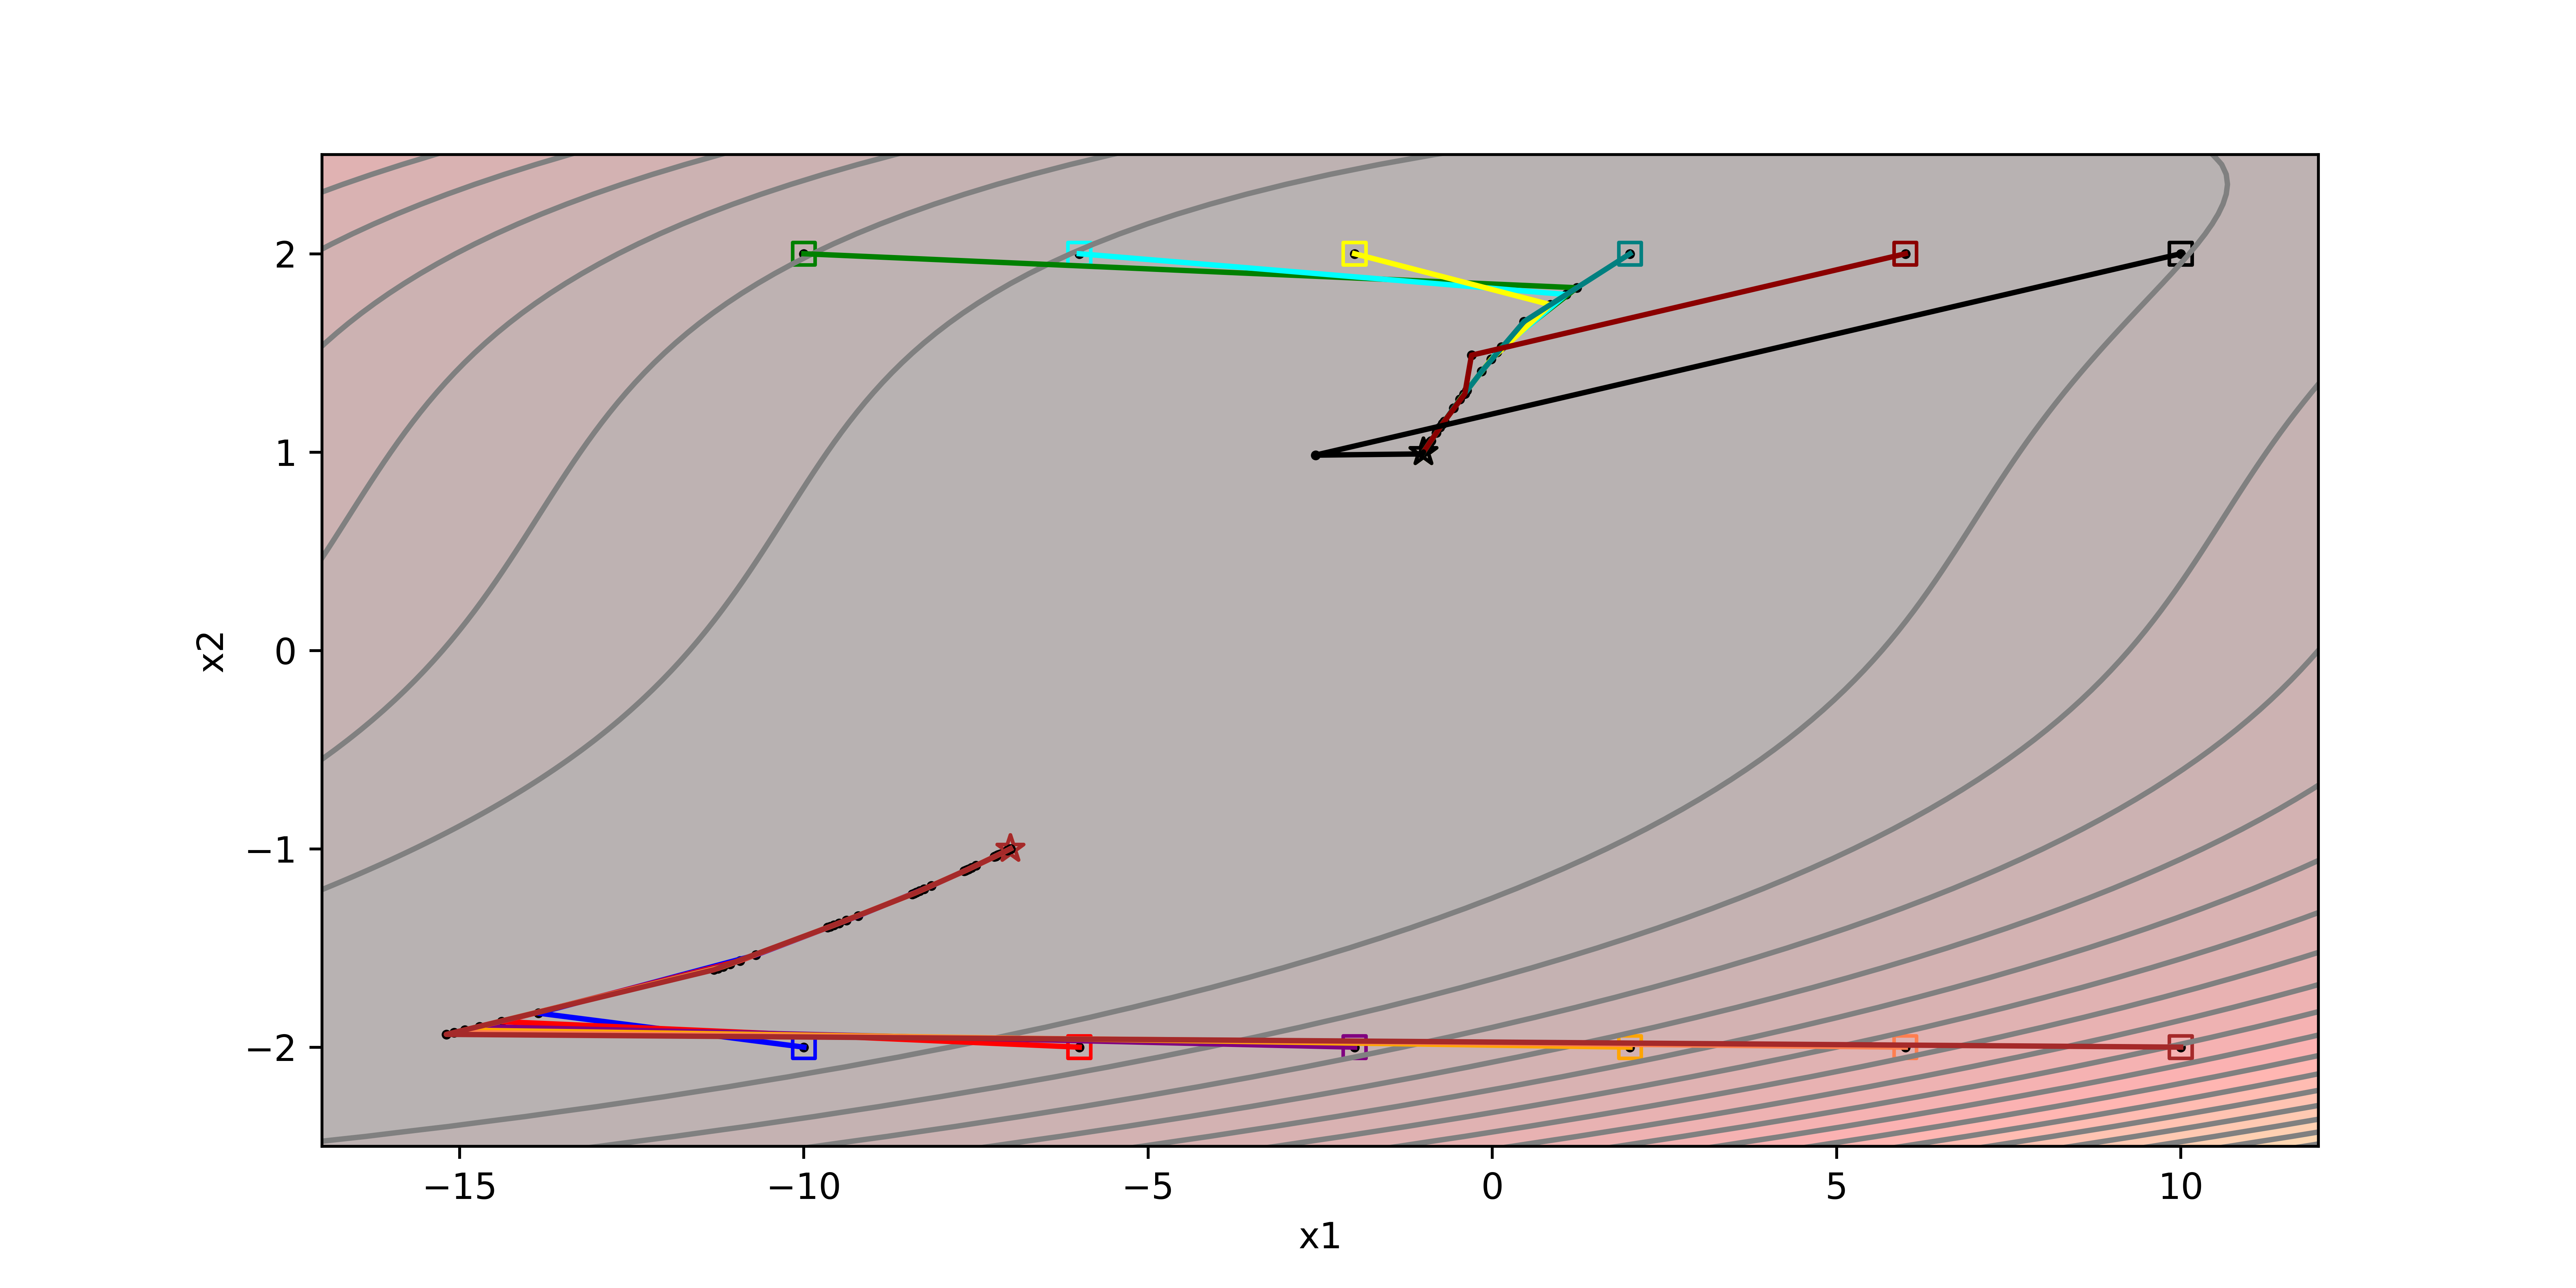
\includegraphics[width=0.6\linewidth]{A4_1_a.png}}
	\quad
	\subfigure[$\log\|x^k-x^*\|$ VS number of iteration]{\label{convergence}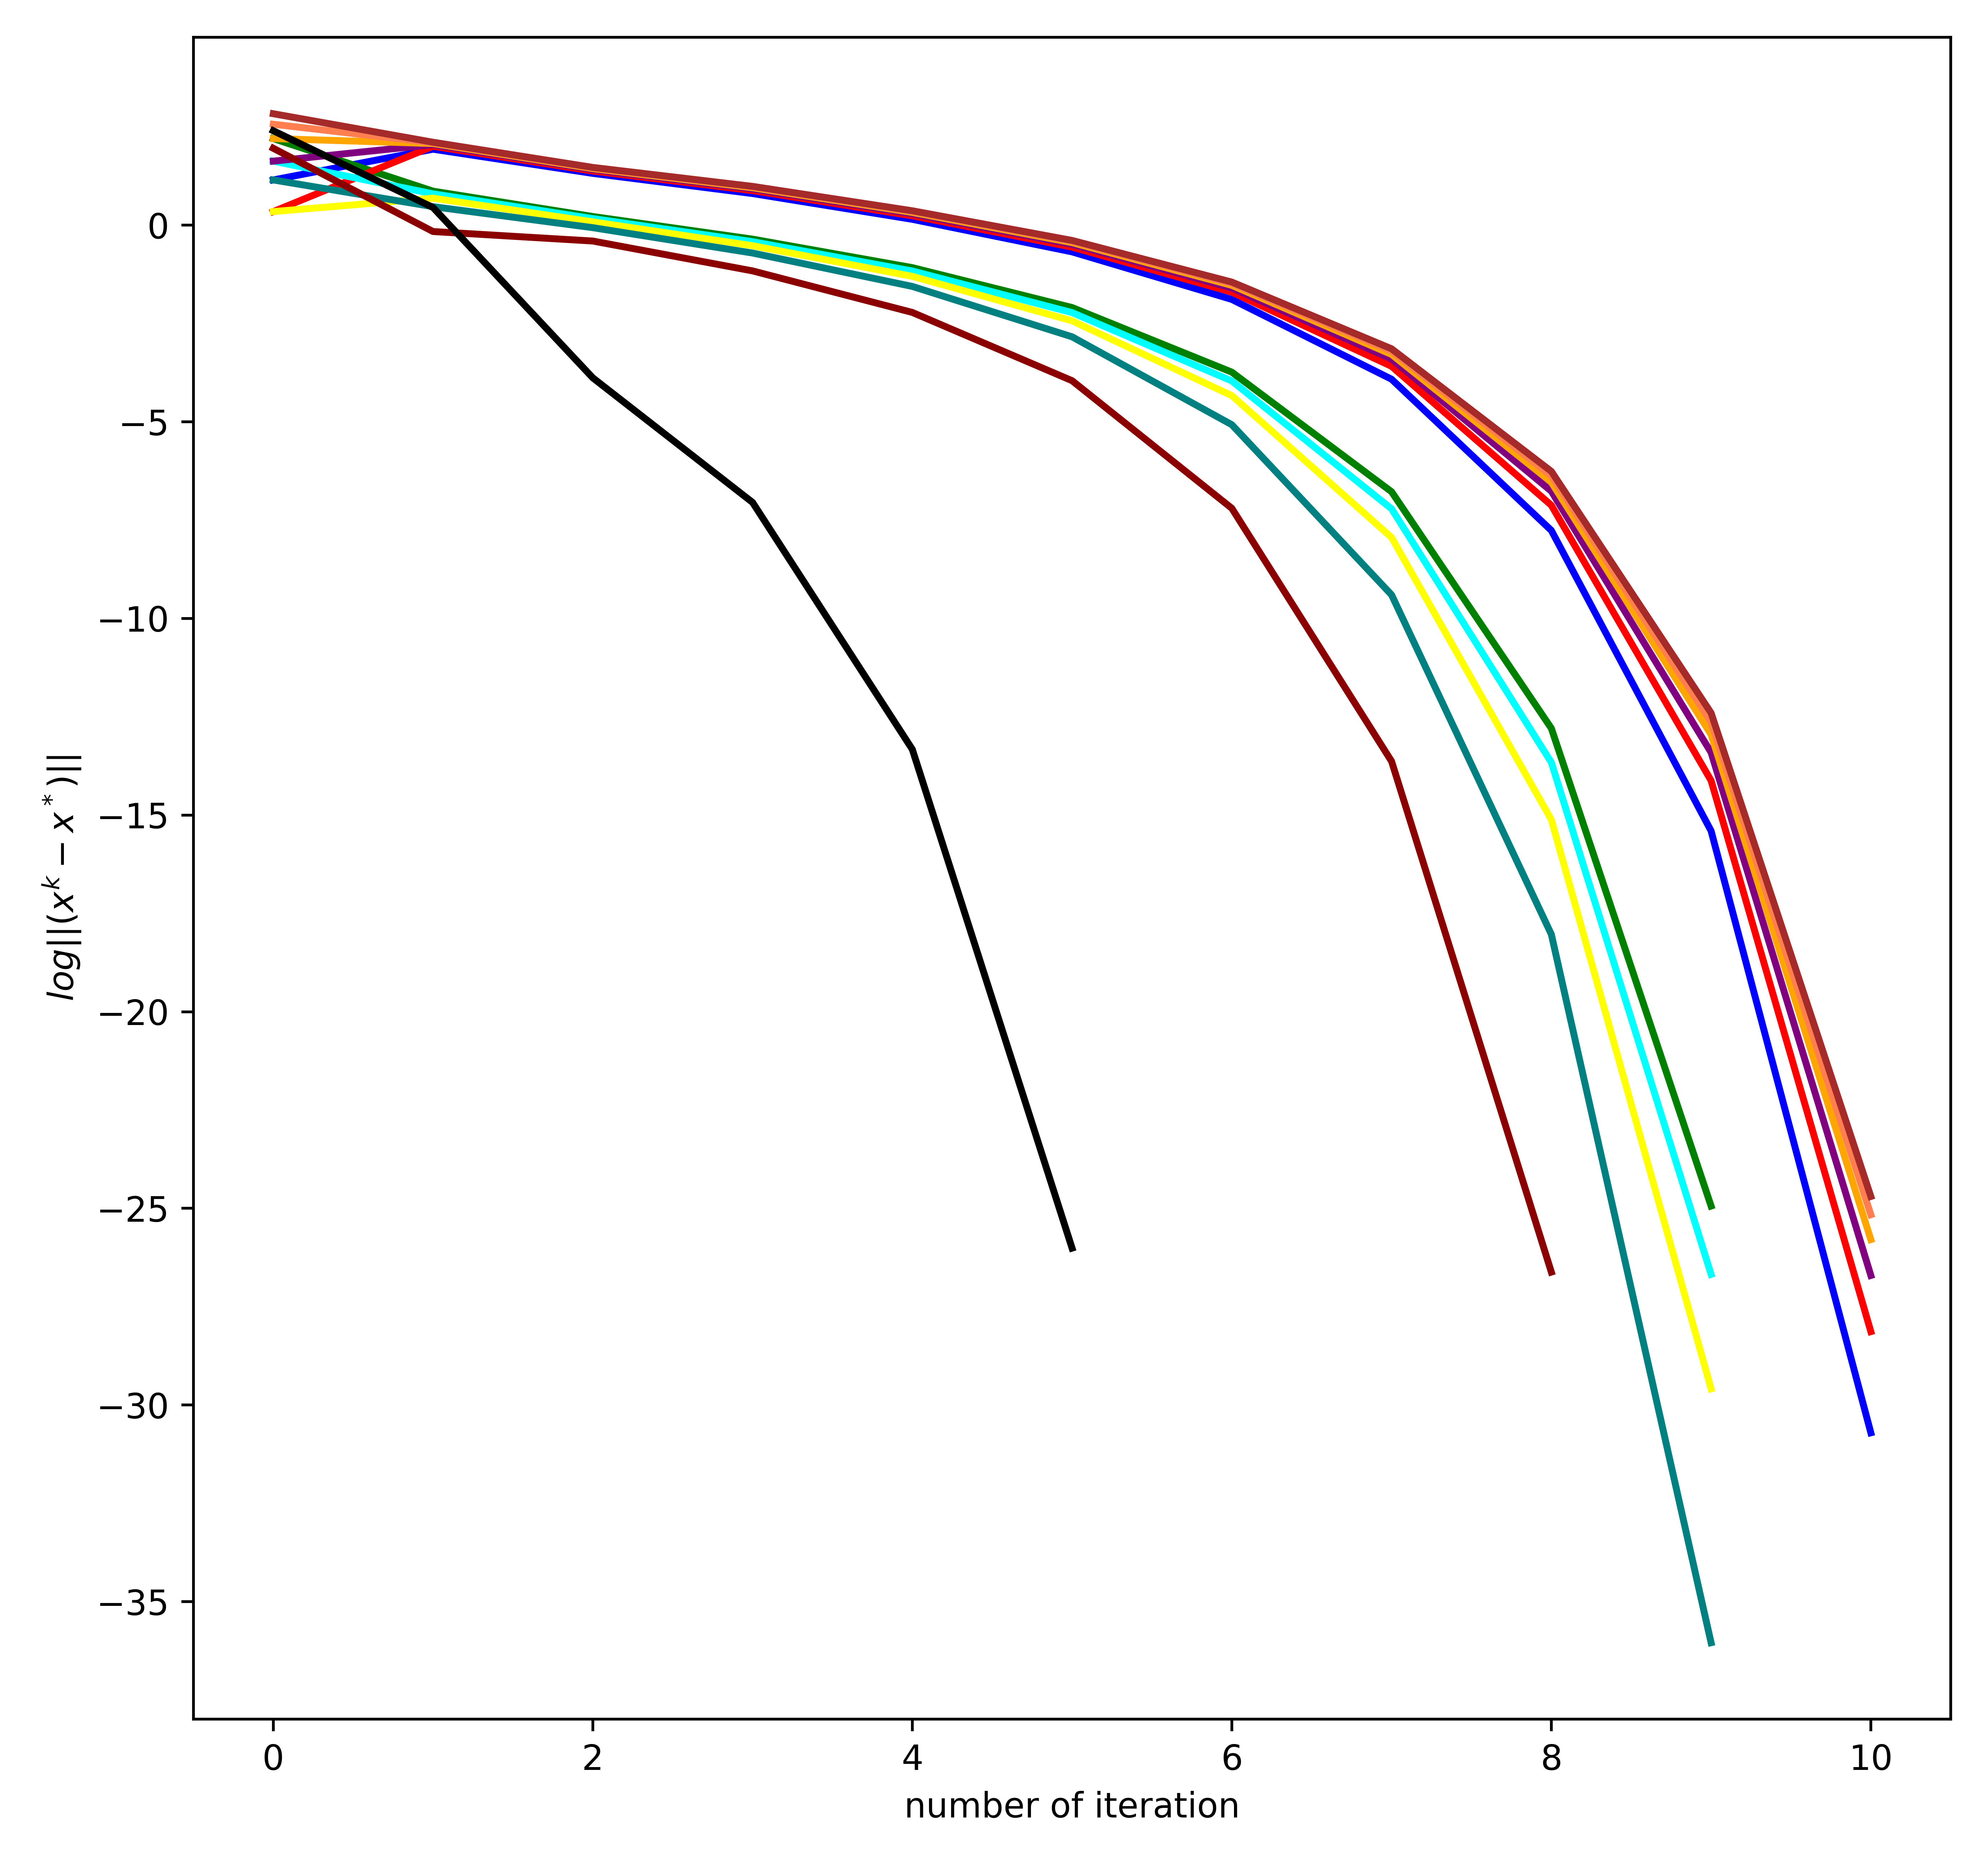
\includegraphics[width=0.35\linewidth]{A4_1_a_convergence.png}}
	\caption{The plot of iteration process}
	\label{gradient}
\end{figure}

By comparing the performance of the Newton method and gradient method tested in A3.3, we can derive Table \ref{performance}. From the table, we can see that the Newton method is much better than the gradient method. The Newton method needs smallest iterations and time.

\begin{table}[htbp]
	\centering  % 显示位置为中间
	\caption{Performance of different methods}  % 表格标题
	\label{performance}  % 用于索引表格的标签
	%字母的个数对应列数,|代表分割线
	% l代表左对齐,c代表居中,r代表右对齐
	\begin{tabular}{|l|c|r|r|}  
		\hline  % 表格的横线
		& & & \\[-6pt]  %可以避免文字偏上来调整文字与上边界的距离
		Method&tolerance&iteration&time(s) \\  % 表格中的内容,用&分开,\\表示下一行
		\hline
		& & & \\[-6pt]  %可以避免文字偏上 
		GM with backtracking &$10^{-8}$&2793&1.613 \\
		& & & \\[-6pt]  %可以避免文字偏上 
		GM with diminishing &$10^{-8}$&85266&8.516 \\
		& & & \\[-6pt]  %可以避免文字偏上 
		GM with exact line search &$10^{-8}$&695&1.007\\
		& & & \\[-6pt]  %可以避免文字偏上 
		Newton method &$10^{-8}$&9&0.035 \\
		\hline
	\end{tabular}
\end{table}

The python code to solve this problem is showing below. 
\begin{python}
import numpy as np
import matplotlib.pyplot as plt
import time

def f1(x):
    x = x.reshape(x.size)
    return 3 + x[0] + ((1 - x[1]) * x[1] - 2) * x[1]
def f2(x):
    x = x.reshape(x.size)
    return 3 + x[0] + (x[1] - 3) * x[1]
def f(x):
    x = x.reshape(x.size)
    return f1(x) * f1(x) + f2(x) *f2(x)
def df(x):
    x = x.reshape(x.size)
    grad = np.zeros(2).reshape(2,1)
    grad[0] = 2 * f1(x) + 2 * f2(x)
    grad[1] = 2 * f1(x) * (2*x[1] - 3*(x[1]**2) - 2) + 2 * f2(x) * (2*x[1] - 3)
    return grad
def Hessian(x):
    x = x.reshape(x.size)
    hessian = np.zeros((2,2))
    hessian[0][0] = 4
    hessian[0][1] = 8*x[1]-6*(x[1]**2)-10
    hessian[1][0] = 8*x[1]-6*(x[1]**2)-10
    hessian[1][1] = 2*f1(x)*(-6*x[1]+2) + 2*(2*x[1]-3*(x[1]**2)-2)**2+4*f2(x)+2*(2*x[1]-3)**2
    return hessian
def norm(x):
    x = x.reshape(x.size)
    return np.sqrt(x[0]**2 + x[1]**2)

color_list = ['blue', 'green', 'red', 'cyan', 'purple', 'yellow', 'orange', 'teal',
              'coral', 'darkred', 'brown', 'black']
Number_iterations = []

def plot_contour():
    X = np.arange(-17.5,12.5,0.05)
    Y = np.arange(-3, 3, 0.05)
    X,Y = np.meshgrid(X,Y)
    Z = np.zeros((X.shape[0], X.shape[1]))
    for i in range(X.shape[0]):
        for j in range(X.shape[1]):
            x = []
            x.append(X[i][j])
            x.append(Y[i][j])
            x = np.array(x)
            Z[i][j] = f(x)
    plt.contourf(X, Y, Z, 30, alpha=0.3, cmap=plt.cm.hot)
    plt.contour(X, Y, Z, 30, colors='grey')
    
def plot_line(xk_list, subfig_num):
    plt.figure(1)
    x = []
    y = []
    for i in range(xk_list.shape[0]):
        x.append(xk_list[i][0][0])
        y.append(xk_list[i][1][0])
    plt.plot(x,y, color = color_list[subfig_num-1], linewidth=1.5)
    plt.scatter(x, y, s=3, color='black')

def plot_convergence(y, subfig_num):
    plt.figure(2, figsize=(8,10))
    n = y.size
    x = np.arange(n)
    y = np.log(y)
    plt.plot(x, y, color = color_list[subfig_num-1], linewidth=2)
    plt.xlabel('number of iteration')
    plt.ylabel('$log||(x^k-x^*)||$')
    plt.tight_layout()

def check_dir(dk_tocheck, xk, gradient, hessian, beta1, beta2):
    dk_norm = norm(dk_tocheck)
    factor1 = np.dot(gradient.T, dk_tocheck)[0][0] < 0
    facotr2 = -(np.dot(gradient.T, dk_tocheck)[0][0]) >= beta1 * np.min([1, dk_norm**beta2]) * dk_norm**2
    if factor1 == True and facotr2 == True:
        return True
    else:
        return False
def Global_Newton(initial, subfig_num):
    #paramaters
    s = 1
    sigma = 0.5
    gamma = 0.1
    beta1 = 1e-6
    beta2 = 0.1
    tol = 1e-8
    xk_list = []
    xk_xstar_list = []


    xk = initial
    num_iteration = 0
    xk_list.append(xk)

    
    gradient = df(xk)
    while norm(gradient) > tol:
        # deteriminate the direction
        hessian = Hessian(xk)
        dk_tocheck = np.linalg.solve(hessian, -gradient)
        good_dir = check_dir(dk_tocheck, xk, gradient, hessian, beta1, beta2)
        if(good_dir == False):
            dk = -gradient
        else:
            dk = dk_tocheck 
        
        alphak = s
        while True:
            if f(xk + alphak*dk) - f(xk) <= gamma * alphak * (np.dot(gradient.T, dk)[0][0]):
                break
            alphak = alphak * sigma
        xk = xk + alphak * dk
        xk_list.append(xk)
        
        gradient = df(xk)
        num_iteration = num_iteration + 1
    
    Number_iterations.append(num_iteration)
    
    plt.figure(1)
    plt.scatter(xk_list[-1][0], xk_list[-1][1], s=60, marker='*', 
                facecolors ='none', edgecolor= color_list[subfig_num-1])
    xk_list = np.array(xk_list)
    plot_line(xk_list, subfig_num)

    xstar_x1 = xk_list[-1][0][0]
    xstar_x2 = xk_list[-1][1][0]
    xstar = np.array([round(xstar_x1), xstar_x2]).reshape(2, 1)
    for i in range(xk_list.shape[0]):
        xk_xstar_list.append(norm(xk_list[i] - xstar))
    xk_xstar_list = np.array(xk_xstar_list)
    plot_convergence(xk_xstar_list, subfig_num)
# main begin

x1 = np.arange(-10, 11, 4)
x2 = np.arange(-2, 3, 4)

plt.figure(1, figsize=(10, 5))
plot_contour()
subfig_num = 1

time_list = []
for i in range(6):
    for j in range(2):
        initial = np.zeros(2).reshape(2,1)
        initial[0][0] = x1[i]
        initial[1][0] = x2[j]
        plt.figure(1)
        plt.scatter(initial[0], initial[1], s=40, marker='s', 
                    facecolors ='none', edgecolor= color_list[subfig_num-1])
        
        start = time.clock()
        Global_Newton(initial, subfig_num)
        end = time.clock()
        
        time_list.append(end - start)
        subfig_num = subfig_num + 1

plt.figure(1)
plt.xlabel('x1')
plt.ylabel('x2')
plt.xlim(-17, 12)
plt.ylim(-2.5, 2.5)
plt.savefig('A4_1_a', dpi=700)  

plt.figure(2)
plt.savefig('A4_1_a_convergence', dpi=700)  

print()
print('Number of iterations from different initial points:', Number_iterations)
print('Average number of iterations from different initial points:', 
      sum(Number_iterations)/len(Number_iterations))

print('Calculating time from different initial points:', time_list)
print('Average calculating time from different initial points:', 
      sum(time_list)/len(time_list))      
\end{python}

\vspace{4pt}
\textbf{Subproblem (b)}

By comparing the performance of the Newton method and gradient method with backtracking, we can derive Table \ref{performance2}. From the table, we can see that the Newton method is much better than the gradient method with backtracking. The Newton method always utilize the Newton direction. Newton method and gradient method both do not always use full step sizes $\alpha_{k}=1$. 
The figures which contains the paths is showing as Figure \ref{path}. The figure of $\left(\log\left\|x^{k}-x^{*}\right\|\right)_{k}$ can be seen in Figure \ref{convergence2}. By zooming in Figure \ref{convergence2}, we get Figure \ref{zoom}. As we can see from the figure, the gradient method is linear convergence, and the Newton method is quadratic convergence. 

\begin{table}[htbp]
	\centering  % 显示位置为中间
	\caption{Performance of different methods on Rosenbrock function}  % 表格标题
	\label{performance2}  % 用于索引表格的标签
	%字母的个数对应列数,|代表分割线
	% l代表左对齐,c代表居中,r代表右对齐
	\begin{tabular}{|l|c|r|r|c|c|}  
		\hline  % 表格的横线
		& & & & &\\[-6pt]  %可以避免文字偏上来调整文字与上边界的距离
		Method&tolerance&iteration&time(s)&always use Newton direction & $\alpha_{k} $ always = 1\\  % 表格中的内容,用&分开,\\表示下一行
		\hline
		\multirow{5}{*}{GM with backtracking}
		& & & & &\\ [-6pt]  %可以避免文字偏上 
		&$10^{-1}$&54&0.050&&False \\
		& & & & &\\[-6pt]  %可以避免文字偏上 
		&$10^{-3}$&5231&1.108&&False  \\
		& & & & &\\[-6pt]  %可以避免文字偏上 
		&$10^{-5}$&10916&2.303&&False \\
		\hline
		\multirow{5}{*}{Newton Method}
		& & & & &\\ [-6pt]  %可以避免文字偏上 
		&$10^{-1}$&19&0.166&True&False  \\
		& & & & &\\[-6pt]  %可以避免文字偏上 
		&$10^{-3}$&20&0.075&True&False  \\
		& & & & &\\[-6pt]  %可以避免文字偏上 
		&$10^{-5}$&21&0.080&True&False \\
		\hline
	\end{tabular}
\end{table}

\begin{figure}[H]
	\centering
	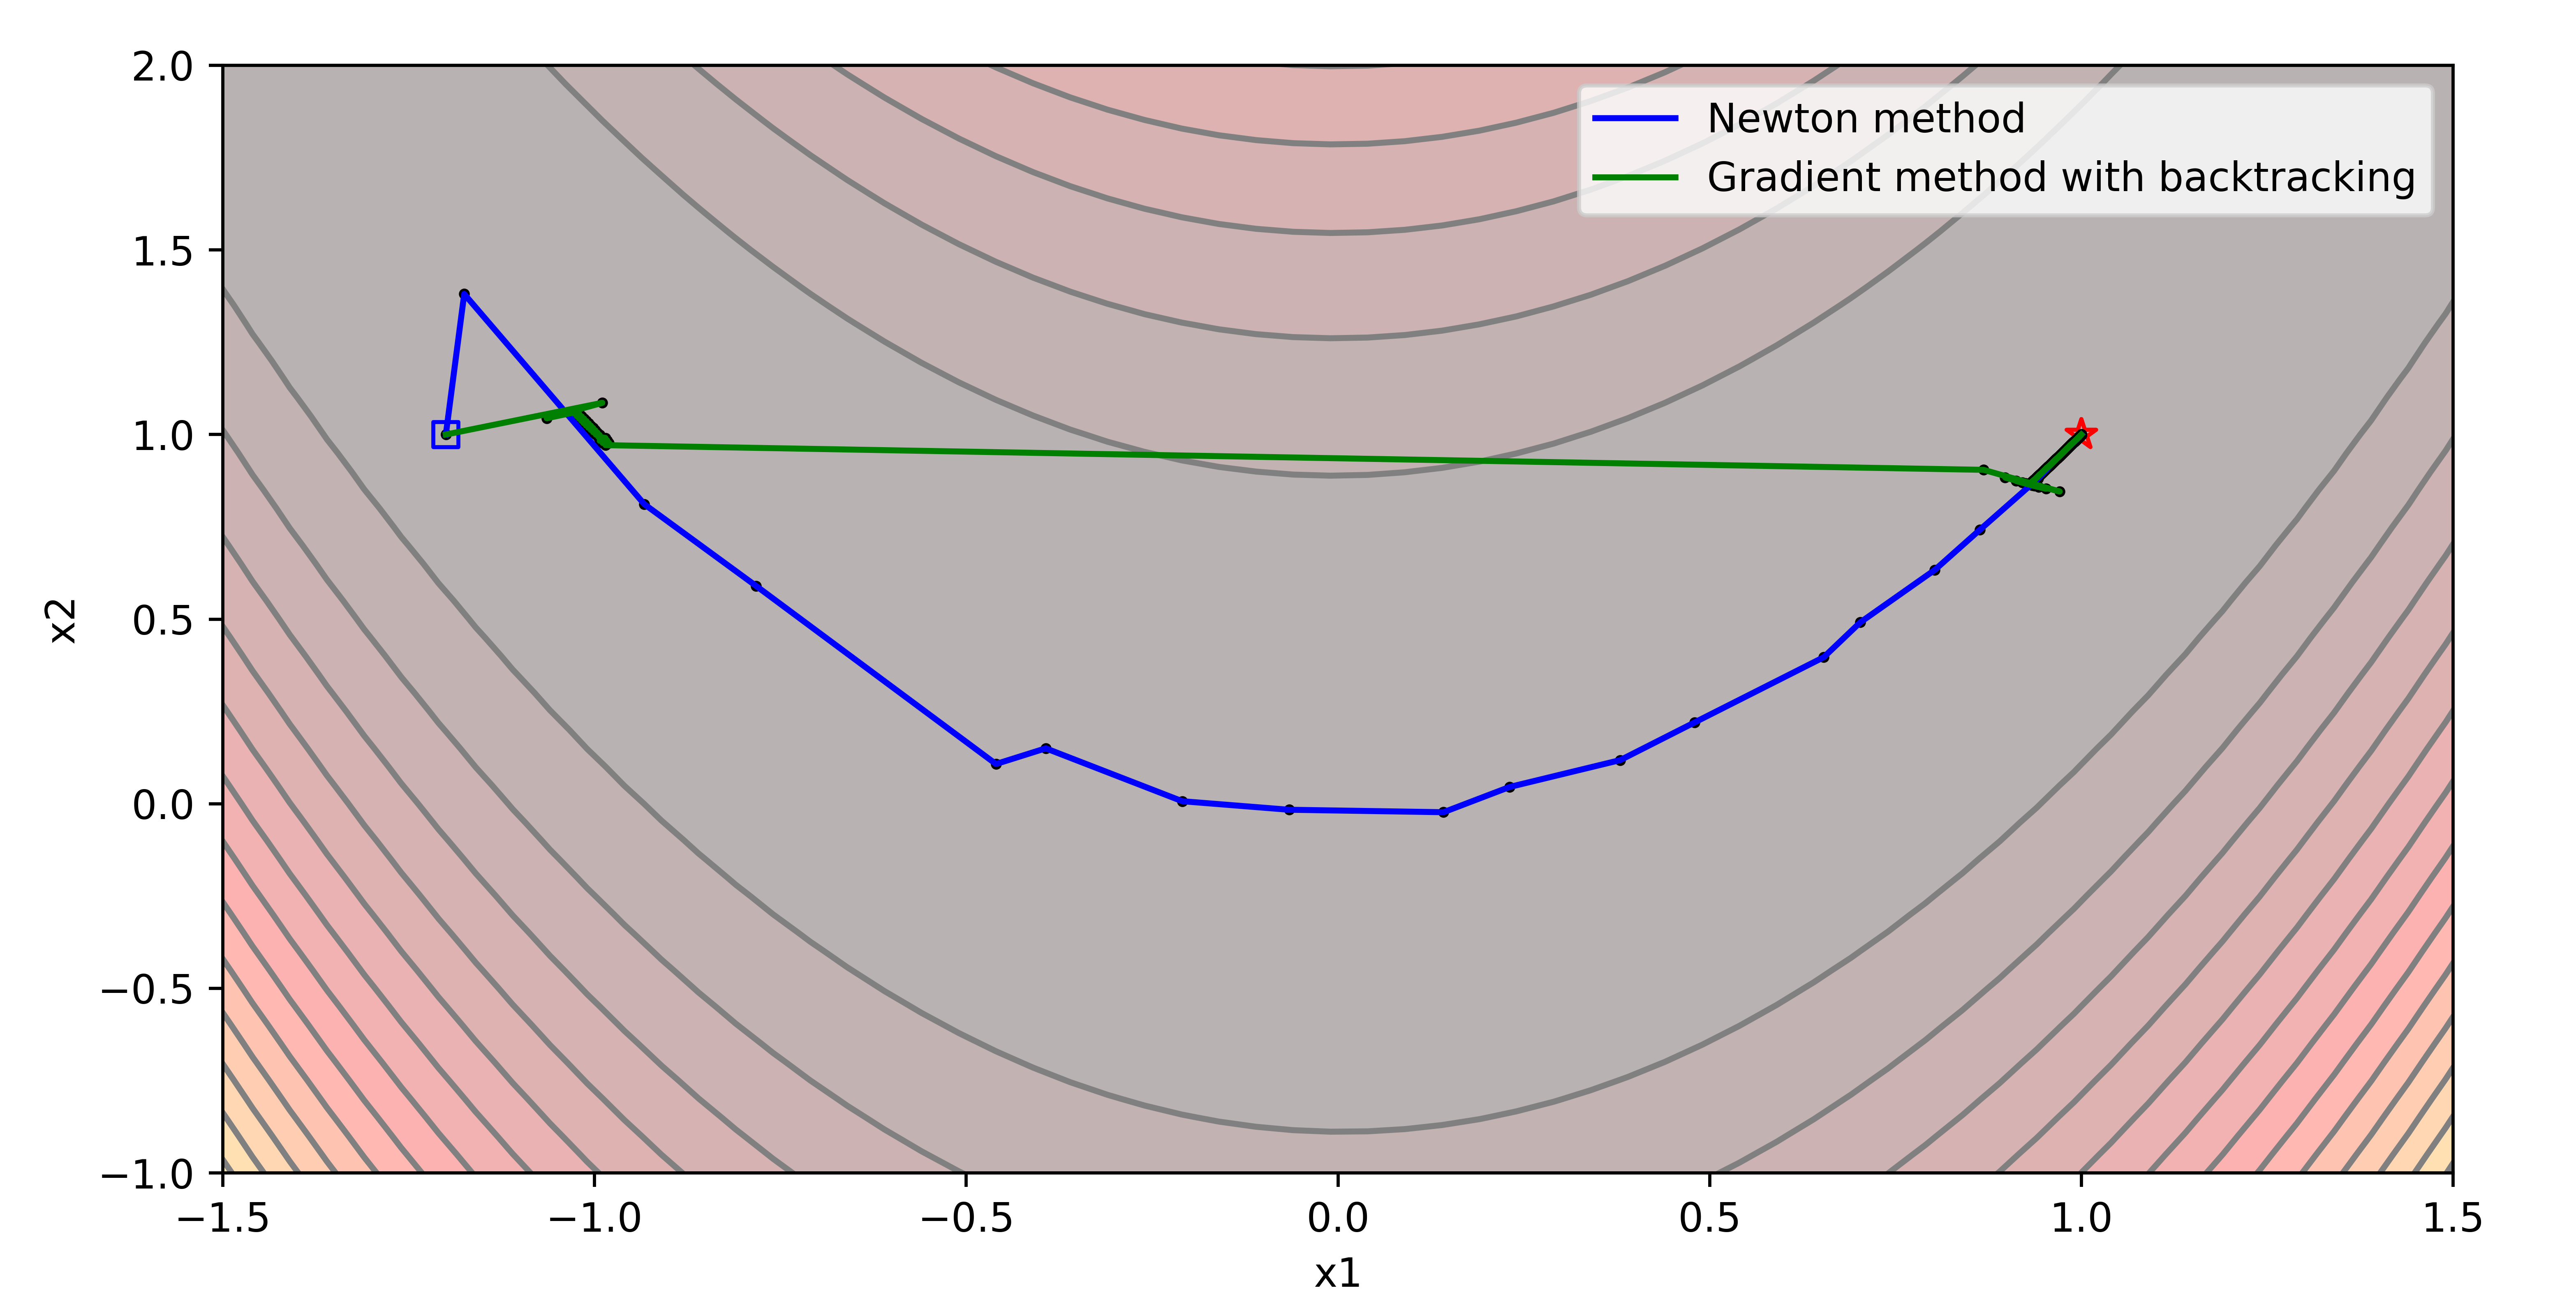
\includegraphics[width=0.7\linewidth]{A4_1_b.png}
	\vspace{-5pt}
	\caption{Paths of Newton method and gradient mothod with backtracking}
	\label{path}
\end{figure}

\begin{figure}[H]
	\centering
	\subfigure[$\log\|x^k-x^*\|$ VS number of iteration]{\label{convergence2}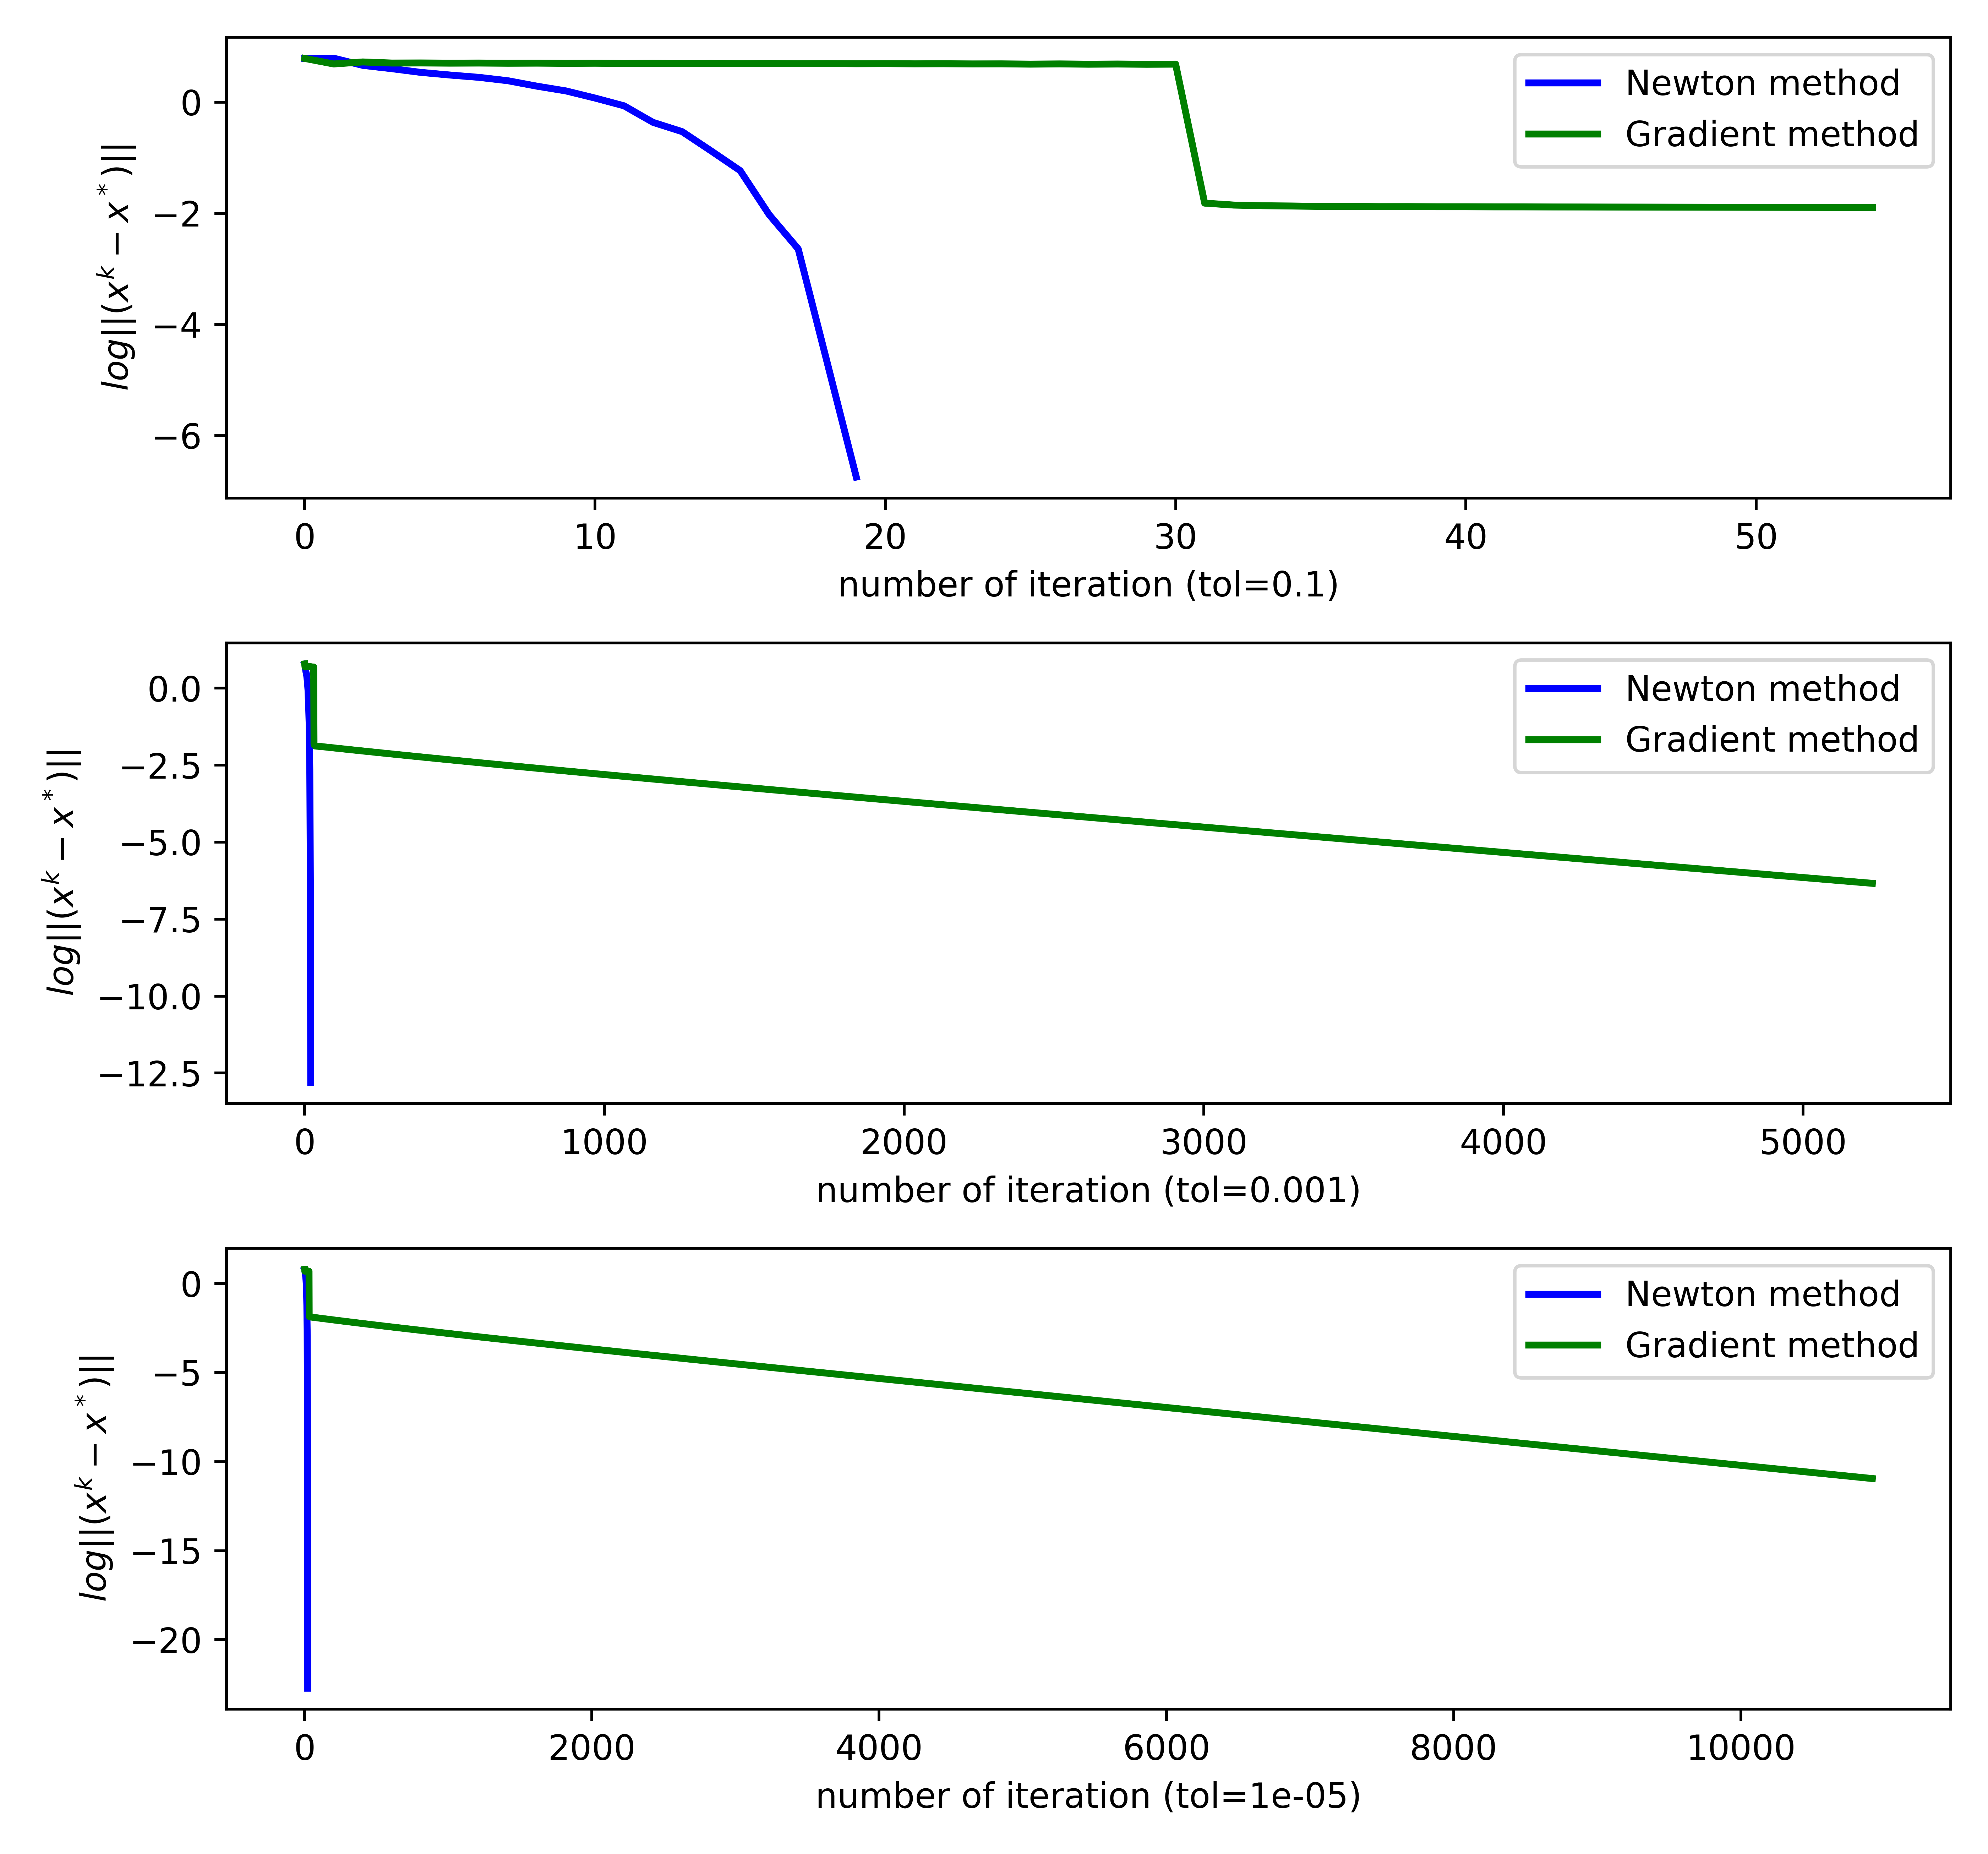
\includegraphics[width=0.41\linewidth]{convergence.png}}
	\quad
	\subfigure[$\log\|x^k-x^*\|$ VS number of iteration (zoom in)]{\label{zoom}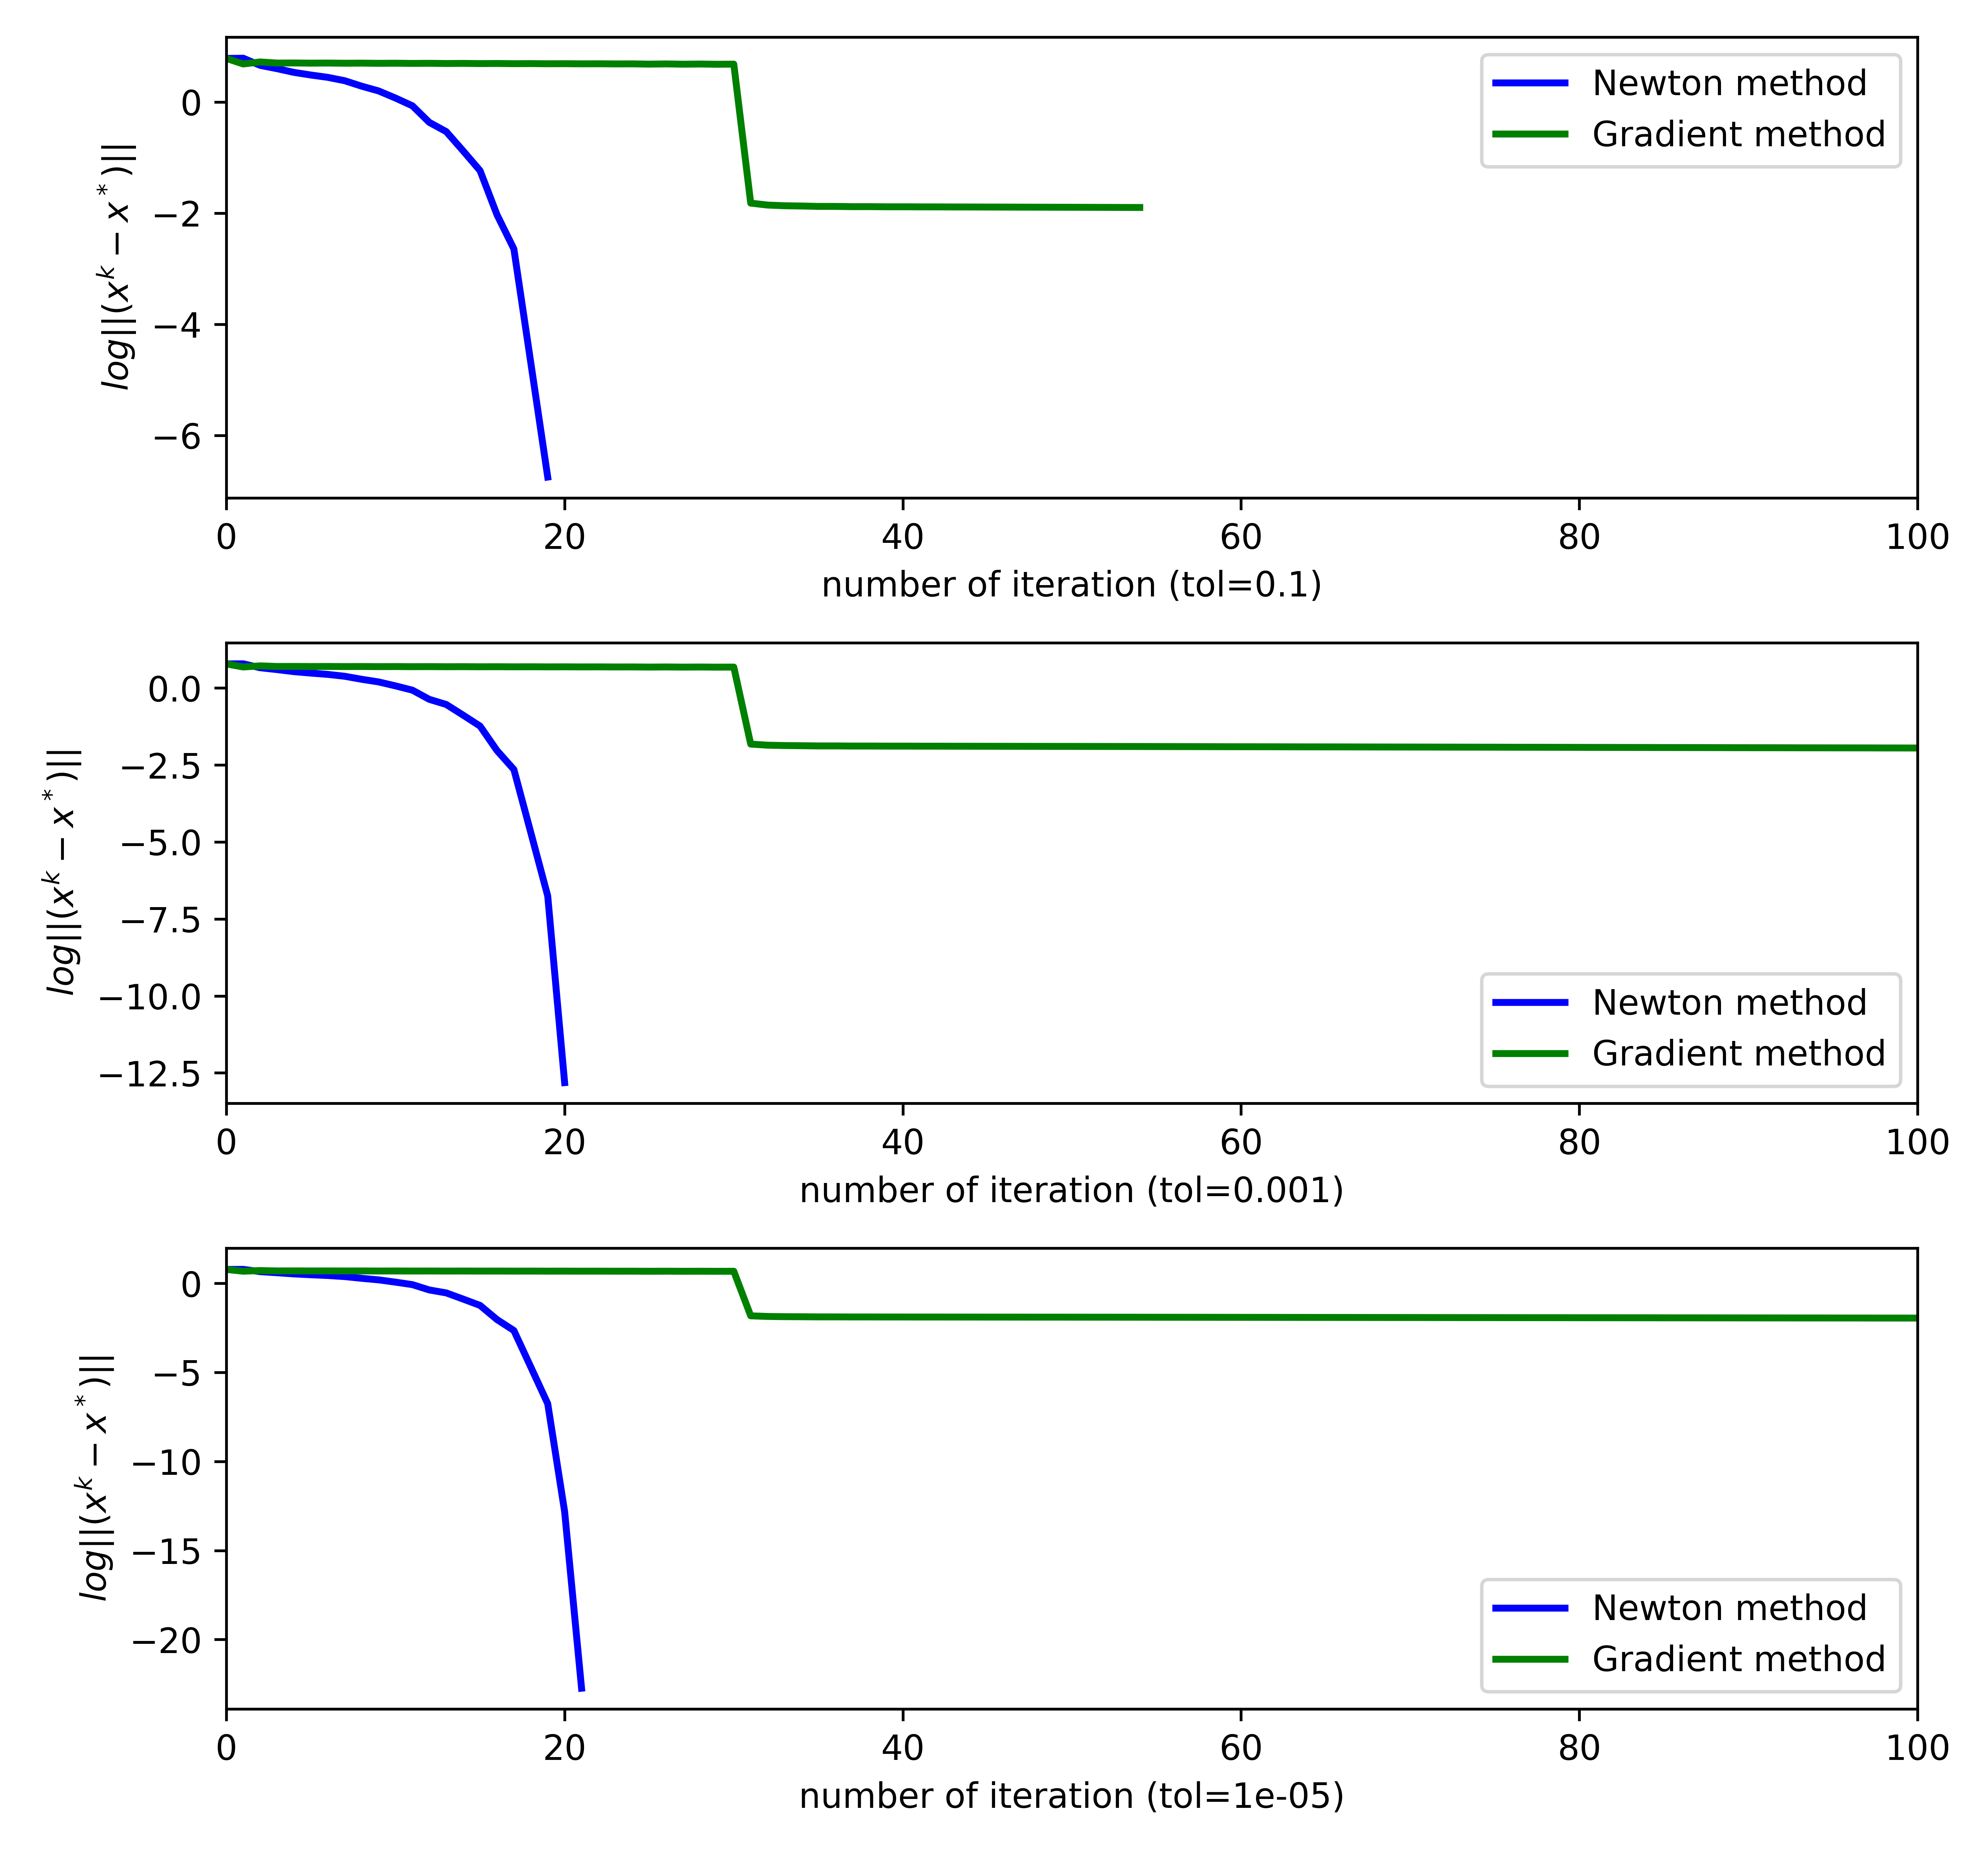
\includegraphics[width=0.41\linewidth]{convergence_zoom.png}}
	\caption{The plot of iteration process}
	\label{gradient}
\end{figure}
The python code to solve this problem is showing below.
\begin{python}
import numpy as np
import matplotlib.pyplot as plt
import time

def f(x): # Rosenbrock function
    x = x.reshape(x.size)
    return 100*(x[1] - x[0]**2)**2 + (1-x[0])**2
def df(x):
    x = x.reshape(x.size)
    grad = np.zeros(2).reshape(2,1)
    grad[0] = -400 * x[0] * (x[1] - x[0]**2) + 2 * x[0] -2
    grad[1] = 200 * (x[1] - x[0]**2)
    return grad
def Hessian(x):
    x = x.reshape(x.size)
    hessian = np.zeros((2,2))
    hessian[0][0] = -400 * (x[1] - 3*x[0]**2) + 2
    hessian[0][1] = -400 * x[0]
    hessian[1][0] =  -400 * x[0]
    hessian[1][1] = 200
    return hessian
def norm(x):
    x = x.reshape(x.size)
    return np.sqrt(x[0]**2 + x[1]**2)

color_list = ['blue', 'green', 'red', 'cyan', 'purple', 'yellow', 'orange', 'teal',
              'coral', 'darkred', 'brown', 'black']
label_list = ['Newton method', 'Gradient method with backtracking']
tol_list = [1e-1, 1e-3, 1e-5]


def plot_contour():
    X = np.arange(-1.51,1.6,0.05)
    Y = np.arange(-1.55, 2.55, 0.05)
    X,Y = np.meshgrid(X,Y)
    Z = np.zeros((X.shape[0], X.shape[1]))
    for i in range(X.shape[0]):
        for j in range(X.shape[1]):
            x = []
            x.append(X[i][j])
            x.append(Y[i][j])
            x = np.array(x)
            Z[i][j] = f(x)
    plt.contourf(X, Y, Z, 20, alpha=0.3, cmap=plt.cm.hot)
    plt.contour(X, Y, Z, 20, colors='grey')
    
def plot_line(xk_list, subfig_num):
    plt.figure(1)
    x = []
    y = []
    for i in range(xk_list.shape[0]):
        x.append(xk_list[i][0][0])
        y.append(xk_list[i][1][0])
    plt.plot(x,y, color = color_list[subfig_num], linewidth=1.5, label=label_list[subfig_num])
    plt.scatter(x, y, s=3, color='black')

def plot_convergence(y, method, subfig_num, tol_index):
    tol_index = tol_index + 1
    plt.figure(2, figsize=(8,10))
    plt.subplot(3,1,tol_index)
    n = y.size
    x = np.arange(n)
    y = np.log(y)
    plt.plot(x, y, label = method, color = color_list[subfig_num], linewidth=2)
    plt.legend()
    plt.xlabel('number of iteration (tol={})'.format(str(tol_list[tol_index-1])))
    plt.ylabel('$log||(x^k-x^*)||$')
    plt.tight_layout()
    #plt.xlim(0,100)
    
def check_dir(dk_tocheck, xk, gradient, hessian, beta1, beta2):
    dk_norm = norm(dk_tocheck)
    factor1 = np.dot(gradient.T, dk_tocheck)[0][0] < 0
    facotr2 = -(np.dot(gradient.T, dk_tocheck)[0][0]) >= beta1 * np.min([1, dk_norm**beta2]) * dk_norm**2
    if factor1 == True and facotr2 == True:
        return True
    else:
        return False
def Global_Newton(initial, subfig_num, tol, tol_index):
    #paramaters
    
    xstar = np.array([1, 1]).reshape(2, 1)
    s = 1
    sigma = 0.5
    gamma = 1e-4
    beta1 = 1e-6
    beta2 = 0.1
    xk_list = []
    xk_xstar_list = []
    alphak_list_Newton = []
    Always_Use_Newton_Dir = True
    
    xk = initial
    num_iteration = 0
    xk_list.append(xk)
    xk_xstar_list.append((norm(xk-xstar)))
    
    gradient = df(xk)
    while norm(gradient) > tol:
        # deteriminate the direction
        hessian = Hessian(xk)
        dk_tocheck = np.linalg.solve(hessian, -gradient)
        good_dir = check_dir(dk_tocheck, xk, gradient, hessian, beta1, beta2)
        if(good_dir == False):
            dk = -gradient
            Always_Use_Newton_Dir = False
        else:
            dk = dk_tocheck 
        
        alphak = s
        alphak_list_Newton.append(alphak)
        
        while True:
            if f(xk + alphak*dk) - f(xk) <= gamma * alphak * (np.dot(gradient.T, dk)[0][0]):
                break
            alphak = alphak * sigma
        alphak_list_Newton.append(alphak)
        xk = xk + alphak * dk
        xk_list.append(xk)
        xk_xstar_list.append((norm(xk-xstar)))
        
        gradient = df(xk)
        num_iteration = num_iteration + 1
    
    print('tolerance:', tol)
    print('Newton_num_iteration:', num_iteration)
    print('Always_Use_Newton_Dir:', Always_Use_Newton_Dir)
    print('alpha_k of Newton method', alphak_list_Newton)
    print()
    
    method = 'Newton method'
    xk_xstar_list = np.array(xk_xstar_list)
    plot_convergence(xk_xstar_list, method, subfig_num, tol_index)
    
    if tol == 1e-5:
        plt.figure(1)
        plt.scatter(xk_list[-1][0], xk_list[-1][1], s=60, marker='*', 
                    facecolors ='none', edgecolor= 'r')
        xk_list = np.array(xk_list)
        plot_line(xk_list, subfig_num)

def gradient_method(initial, subfig_num, tol, tol_index):
    xstar = np.array([1, 1]).reshape(2, 1)
    s = 1
    sigma = 0.5
    gamma = 1e-4
    xk_list = []
    xk_xstar_list = []
    alphak_list_GM = []

    
    xk = initial
    gradient = df(xk)
    num_iteration = 0
    xk_list.append(xk)
    xk_xstar_list.append((norm(xk-xstar)))
    
    while norm(gradient) > tol:
        alphak = s
        alphak_list_GM.append(alphak)
        
        dk = -df(xk)
        while True:
            if f(xk + alphak*dk) - f(xk) <= gamma * alphak * (np.dot(df(xk).T, dk)[0][0]):
                break
            alphak = alphak * sigma
            
        alphak_list_GM.append(alphak)
        xk = xk + alphak * dk
        xk_list.append(xk)
        xk_xstar_list.append((norm(xk-xstar)))
        
        gradient = df(xk)
        num_iteration = num_iteration + 1
    
    print('tolerance:', tol)
    print('Gradient_mothd_num_iteration:', num_iteration)
    print('alpha_k of GM method', alphak_list_GM)
    print()
    
    method = 'Gradient method'
    xk_xstar_list = np.array(xk_xstar_list)
    plot_convergence(xk_xstar_list, method, subfig_num, tol_index)
    
    if tol == 1e-5:
        plt.figure(1)
        plt.scatter(xk_list[-1][0], xk_list[-1][1], s=60, marker='*', 
                facecolors ='none', edgecolor= 'r')
        xk_list = np.array(xk_list)
        plot_line(xk_list, subfig_num)
        
# main begin

x1 = np.arange(-10, 11, 4)
x2 = np.arange(-2, 3, 4)

plt.figure(1, figsize=(10, 5))
plot_contour()

initial = np.array([[-1.2], [1]])
plt.figure(1)
plt.scatter(initial[0], initial[1], s=40, marker='s', 
                    facecolors ='none', edgecolor= 'b')

print('----------Newton Method----------')
for index, tol in enumerate(tol_list):
    
    start = time.clock()
    Global_Newton(initial, 0, tol, index)
    end = time.clock()
    
    print('time:', end - start)
    print()
    
print('----------Gradient Method----------')
for index, tol in enumerate(tol_list):
    
    start = time.clock()
    gradient_method(initial, 1, tol, index)
    end = time.clock()
    
    print('time:', end - start)
    print()

plt.figure(1)
plt.xlabel('x1')
plt.ylabel('x2')
plt.xlim(-1.5, 1.5)
plt.ylim(-1, 2)
plt.legend()
plt.show()
plt.savefig('A4_1_b', dpi=700)

plt.figure(2)
plt.savefig('convergence', dpi=700)
\end{python}
\end{homeworkProblem}

\pagebreak
\begin{homeworkProblem}
In this exercise, we consider the $\ell_{1}$ -optimization problem
$$
\min _{x} f(x)=\frac{1}{2}\|A x-b\|^{2}+\mu\|x\|_{1}
$$
where $A \in \mathbb{R}^{m \times n}, b \in \mathbb{R}^{m}$ and $\mu>0$ are given. In order to handle the nonsmoothness of the $\ell_{1}$ -norm, we substitute $\varphi(x)=\|x\|_{1}$ in (1) with one of the following smooth options:
$$
\varphi_{1}(x)=\|x\|_{2}^{2}, \quad \varphi_{2}(x)=\sum_{i=1}^{n} \varphi_{\mathrm{hub}}\left(x_{i}\right), \quad \text { and } \quad \varphi_{3}(x)=\sum_{i=1}^{n} \varphi_{\log }\left(x_{i}\right)
$$
where
$$
\varphi_{\text {hub }}(t):=\left\{\begin{array}{ll}
\frac{1}{2 \delta} t^{2} & \text { if }|t| \leq \delta \\
|t|-\frac{1}{2} \delta & \text { if }|t|>\delta
\end{array} \quad\right. \text { and } \quad\varphi_{\log }(t):=\log \left(1+t^{2} / \nu\right), \quad \delta, \nu>0
$$
The data $A$ and $b$ is generated as follows: choose $n, m, s \in \mathbb{N}$ with $s \leq m \leq n$ and create a mask mask $=$ randperm $(\mathrm{n}, \mathrm{s}) .($ The vector mask contains $s$ different integers from 1 to $n) .$ We then construct a sparse signal $x^{*} \in \mathbb{R}^{n}$ via
$$
x^{*}=\operatorname{zeros}(\mathrm{n}, 1) \quad x^{*}(\operatorname{mask})=\operatorname{randn}(\mathrm{s}, 1)
$$
Hence, $x^{*}$ is an $n$ -dimensional vector with $s$ -nonzero (randomly selected) entries that follow a Normal distribution. We choose $A=\operatorname{randn}(\mathrm{m}, \mathrm{n})$ and generate the partial measurements $b$ via $b=A x^{*}+0.01 \cdot \operatorname{randn}(\mathrm{m}, 1) .$ The goal is to reconstruct the original sparse signal $x^{*}$ from the much smaller measurements $b$ via solving the problem (1) and its smooth variants.
\begin{enumerate}[a)]
	\item  Implement the accelerated gradient method (Lecture L-09, slide 29) for problem (1) using $\varphi_{1}$ and $\varphi_{2} .$ The extrapolation parameter and step size should be chosen as follows:
	$$
	\alpha_{k}=\frac{1}{L}, \quad \beta_{k}=\frac{t_{k-1}-1}{t_{k}}, \quad t_{k}=\frac{1}{2}\left(1+\sqrt{1+4 t_{k-1}^{2}}\right), \quad t_{-1}=t_{0}=1
	$$
	Here, $L$ denotes the Lipschitz constants of the gradient mappings $\nabla f_{1}(x)=A^{\top}(A x-b)+$ $\nabla \varphi_{1}(x)$ and $\nabla f_{2}(x)=A^{\top}(A x-b)+\nabla \varphi_{2}(x),$ respectively. It can be shown that the two constants are given by
	$$
	L_{1}=2 \mu+\left\|A^{\top} A\right\|\left(\text { for } \nabla f_{1}\right) \quad \text { and } \quad L_{2}=\mu \delta^{-1}+\left\|A^{\top} A\right\|\left(\text { for } \nabla f_{2}\right)
	$$
	\item Implement the inertial gradient method (Lecture $\mathrm{L}-09,$ slide 42 ) for problem (1) using $\varphi_{1}$, $\varphi_{2},$ and $\varphi_{3} .$ Here, you can implement the following variant for unknown Lipschitz constant:
	
	\begin{tabular}{ll}
		\toprule
		 & \textbf{Algorithm 1: The Inertial Gradient Method for Unknown Lipschitz Constants}\\
		\midrule
		\textbf{1} &  Initialization: Choose an initial point $x^{0} \in \mathbb{R}^{n},$ set $x^{-1}=x^{0}, \beta \in[0,1), \ell>0,$ and calculate\\
		& $\alpha=1.99(1-\beta) / \ell$\\
		&  	\textbf{for} $k=0,1,2, \ldots$ \textbf{do}\\
		\textbf{2}& Compute $y^{k+1}=x^{k}+\beta\left(x^{k}-x^{k-1}\right)$ and set $\bar{x}^{k+1}=y^{k+1}-\alpha \nabla f\left(x^{k}\right)$\\
		\textbf{3}&\textbf{while} $f\left(\bar{x}^{k+1}\right)-f\left(x^{k}\right)>\nabla f\left(x^{k}\right)^{\top}\left(\bar{x}^{k+1}-x^{k}\right)+\frac{\ell}{2}\left\|\bar{x}^{k+1}-x^{k}\right\|^{2}$ \textbf{do}\\
		&Set $\ell=2 \cdot \ell$ and $\alpha=1.99(1-\beta) / \ell$ and recompute $\bar{x}^{k+1}=y^{k+1}-\alpha \nabla f\left(x^{k}\right)$\\
		\textbf{4}&Set $x^{k+1} = \bar{x}^{k+1}$\\
		\bottomrule
	\end{tabular}
	\item Test your implementations for $m=300, n=3000,$ and $s=30 .$ Report and compare the performance of the methods using the different sparse models. For $f_{1}$ and $f_{2}$ you can choose $\mu \in[0.1,10]$ and $\delta \in\left[10^{-5}, 10^{-3}\right] ;$ for $f_{3}$ you can set $\mu \in\left[10^{-3}, 10^{-1}\right]$ and $\nu \in\left[10^{-5}, 10^{-4}\right]$.
	You can select $x^{0}=0$ as initial point and tol $=10^{-4}$. (Performance can be measured by comparing $\left\|\nabla f\left(x^{k}\right)\right\|$ or $\left|f\left(x^{k}\right)-f^{*}\right| / \max \left\{1,\left|f^{*}\right|\right\}$ where $f^{*}$ is an approximation of the optimal objective function value).
		
	Plot the reconstructed solutions and compare them with the true solution $x^{*}$. Check whether your solutions are truly sparse - which of the models and algorithms performed best in these tasks?

\end{enumerate}

\pagebreak


\vspace{4pt}
\textbf{\large{Solution}}

\vspace{4pt}
\textbf{Subproblem (a)}

The python code to solve this problem is showing below.
\begin{python}
import numpy as np
import matplotlib.pyplot as plt
import time

def norm(x):
    x = x.reshape(x.size)
    return np.sqrt(np.sum(x**2))

def norm_square(x):
    x = x.reshape(x.size)
    return np.sum(x**2)

def huber(t):
    if np.abs(t) <= delta:
        return (t**2) / (2*delta)
    else:
        return np.abs(t) - delta/2

def d_huber(t):
    if np.abs(t) <= delta:
        return t/delta
    else:
        return t/np.abs(t)

def log_fun(t):
    return np.log(1 + t**2/v) 

def d_log_fun(t):
    return (1/(1+t**2/v)) * (2*t/v)
    
def phi_1(x):
    return norm_square(x)

def d_phi_1(x):
    grad = 2*x
    return grad

def phi_2(x):
    x = x.reshape(x.size)
    Sum = 0
    for xi in x:
        Sum = Sum + huber(xi)
    return Sum

def d_phi_2(x):
    x = x.reshape(x.size)
    grad = np.zeros((x.size,1))
    for i in range(grad.size):
        grad[i] = d_huber(x[i])
    return grad

    
def phi_3(x):
    x = x.reshape(x.size)
    Sum = 0
    for xi in x:
        Sum = Sum + log_fun(xi)
    return Sum

def d_phi_3(x):
    x = x.reshape(x.size)
    grad = np.zeros((x.size,1))
    for i in range(grad.size):
        grad[i] = d_log_fun(x[i])
    return grad

color_list = ['blue', 'green', 'red', 'cyan', 'purple', 'yellow', 'orange', 'teal',
              'coral', 'darkred', 'brown', 'black']
def plot_convergence(y, method, subfig_num, tol):
    plt.figure(1)
    plt.subplot(2,1,subfig_num)
    n = y.size
    x = np.arange(n)
    y = np.log(y)
    plt.plot(x, y, label = method, color = color_list[subfig_num], linewidth=2)
    plt.legend()
    plt.xlabel('number of iteration (tol={})'.format(tol))
    plt.ylabel('$log||gradient||$')
    plt.tight_layout()

def plt_compare_and_sparse(x_solution, subfig_num):
    plt.figure(subfig_num+1, figsize=(8,20))
    plt.subplot(2,1,1)
    plt.scatter(x_solution, x_star, color=color_list[0], s=2)
    xmin = x_solution.min()
    xmax = x_solution.max()
    
    plt.plot([x_star.min(), x_star.max()], [x_star.min(), x_star.max()], '--', color='red', linewidth=1, label='diagonal line')
    plt.xlim(xmin-0.02, xmax+0.01)
    plt.xlabel('Solution')
    plt.ylabel('$x^*$')
    plt.legend()
    
    plt.subplot(2,1,2)
    n = x_solution.size
    plt.plot([0,n], [0,0], '--', color='red', linewidth=1)
    plt.scatter(np.arange(n)+1, x_solution, color=color_list[1], s=2)
    plt.xlabel('$i$ (the $i^{th}$ unit of solution)')
    plt.ylabel('The value of $i^{th}$ unit in solution')

    plt.tight_layout()
    plt.savefig('compare_f' +str(subfig_num), dpi=700)
    
    
def f1(x):
    return 1/2 * norm_square(np.dot(A,x) - b) + mu * phi_1(x)

def f2(x):
    return 1/2 * norm_square(np.dot(A,x) - b) + mu * phi_2(x)

def f3(x):
    return 1/2 * norm_square(np.dot(A,x) - b) + mu * phi_3(x)

def df1(x):
    return np.dot(A.T, np.dot(A, x)-b) + mu * d_phi_1(x)
    
def df2(x):
    return np.dot(A.T, np.dot(A, x)-b) + mu * d_phi_2(x)

def df3(x):
    return np.dot(A.T, np.dot(A, x)-b) + mu * d_phi_3(x)

def AGM(initial, smooth_func_type):
    if smooth_func_type == 1:
        df = df1
        alpha_k = 1 / L1
        method = 'AGM method on $f_1$'
    elif smooth_func_type == 2:
        df = df2
        alpha_k = 1 / L2
        method = 'AGM method on $f_2$'
        
    tol = 1e-4  # vary
    x_minus = initial
    xk = initial
    
    tk_minus = 1
    tk = 1
    
    xk_list = []
    xk_list.append(xk)
    norm_gradient_list = []
    num_iteration = 0
     
    gradient = df(xk)
    norm_gradient_list.append(norm(gradient))
    
    while norm(gradient) > tol:
        beta_k = (tk_minus - 1)/tk
        y = xk + beta_k * (xk - x_minus)
        
        x_minus = xk
        xk = y - alpha_k * df(y)
        xk_list.append(xk)
        
        tk_minus = tk
        tk = 1/2 * (1 + np.sqrt(1+4*tk**2))
        
        gradient = df(xk)
        norm_gradient_list.append(norm(gradient))
        # print(norm(gradient))
        num_iteration  = num_iteration + 1
    
    xk_list = np.array(xk_list)
    print(xk_list.shape)
    norm_gradient_list = np.array(norm_gradient_list)
    plot_convergence(norm_gradient_list, method, smooth_func_type, tol)
    
    x_solution = xk_list[-1]
    print('norm of (xk-x_star):', norm(x_solution - x_star))
    plt_compare_and_sparse(x_solution, smooth_func_type)
    

# main begin    
#parameters

np.random.seed(2222)
n = 3000
m = 300
s = 30
mu = 1
delta = 1e-3
v = 1e-5

A = np.random.randn(m, n)
mask = np.random.choice(np.arange(1,n+1), s, replace=False)
x_star = np.zeros((n,1))
for i in range(n):
    if i+1 in mask:
        x_star[i][0] = np.random.randn(1)[0]

b = np.dot(A, x_star) + 0.01 * np.random.randn(m, 1)
L1 = 2*mu + np.linalg.norm(np.dot(A.T, A), ord = 2)
L2 = mu*(1/delta) + np.linalg.norm(np.dot(A.T, A), ord = 2)

initial = np.zeros((n,1))

plt.figure(1, figsize=(8,12))

print('----------f1----------')
start = time.clock()
AGM(initial, 1)
end = time.clock()
print('time:', end - start)
print()

print('----------f2----------')
start = time.clock()
AGM(initial, 2)
end = time.clock()
print('time:', end - start)
print()

plt.figure(1)
plt.savefig('4_2_a_convergence.png', dpi=700)
\end{python}

\vspace{4pt}
\textbf{Subproblem (b)}

The python code to solve this problem is showing below.
\begin{python}
import numpy as np
import matplotlib.pyplot as plt
import time

def norm(x):
    x = x.reshape(x.size)
    return np.sqrt(np.sum(x**2))

def norm_square(x):
    x = x.reshape(x.size)
    return np.sum(x**2)

def huber(t):
    if np.abs(t) <= delta:
        return (t**2) / (2*delta)
    else:
        return np.abs(t) - delta/2

def d_huber(t):
    if np.abs(t) <= delta:
        return t/delta
    else:
        return t/np.abs(t)

def log_fun(t):
    return np.log(1 + t**2/v) 

def d_log_fun(t):
    return (1/(1+t**2/v)) * (2*t/v)
    
def phi_1(x):
    return norm_square(x)

def d_phi_1(x):
    grad = 2*x
    return grad

def phi_2(x):
    x = x.reshape(x.size)
    Sum = 0
    for xi in x:
        Sum = Sum + huber(xi)
    return Sum

def d_phi_2(x):
    x = x.reshape(x.size)
    grad = np.zeros((x.size,1))
    for i in range(grad.size):
        grad[i] = d_huber(x[i])
    return grad

def phi_3(x):
    x = x.reshape(x.size)
    Sum = 0
    for xi in x:
        Sum = Sum + log_fun(xi)
    return Sum

def d_phi_3(x):
    x = x.reshape(x.size)
    grad = np.zeros((x.size,1))
    for i in range(grad.size):
        grad[i] = d_log_fun(x[i])
    return grad
def f1(x):
    return 1/2 * norm_square(np.dot(A,x) - b) + mu * phi_1(x)

def f2(x):
    return 1/2 * norm_square(np.dot(A,x) - b) + mu * phi_2(x)

def f3(x):
    return 1/2 * norm_square(np.dot(A,x) - b) + mu * phi_3(x)

def df1(x):
    return np.dot(A.T, np.dot(A, x)-b) + mu * d_phi_1(x)
    
def df2(x):
    return np.dot(A.T, np.dot(A, x)-b) + mu * d_phi_2(x)

def df3(x):
    return np.dot(A.T, np.dot(A, x)-b) + mu * d_phi_3(x)

color_list = ['brown', 'green', 'red', 'blue', 'cyan', 'purple', 'yellow', 'orange', 'teal',
              'coral', 'darkred', 'black']
def plot_convergence(y, method, subfig_num, tol, knownL):
    plt.figure(2-knownL)
    
    if knownL == True:
        sum_fig = 2
    else:
        sum_fig = 3
    plt.subplot(sum_fig, 1, subfig_num)
    n = y.size
    x = np.arange(n)
    y = np.log(y)
    plt.plot(x, y, label = method, color = color_list[subfig_num], linewidth=2)
    plt.legend()
    plt.xlabel('number of iteration (tol={})'.format(tol))
    plt.ylabel('$log||gradient||$')
    plt.tight_layout()

def plt_compare_and_sparse(x_solution, subfig_num, knownL):
    if knownL == True:
        Type = 'knwonL'
        fignum_begin = 3
    else:
        Type = 'UnknownL'
        fignum_begin = 5
        
    plt.figure(fignum_begin + subfig_num - 1, figsize=(8,20))
    plt.subplot(2,1,1)
    plt.scatter(x_solution, x_star, color=color_list[3], s=2)
    xmin = x_solution.min()
    xmax = x_solution.max()
    
    plt.plot([x_star.min(), x_star.max()], [x_star.min(), x_star.max()], '--', color='red', linewidth=1, label='diagonal line')
    plt.xlim(xmin-0.02, xmax+0.01)
    plt.xlabel('Solution')
    plt.ylabel('$x^*$')
    plt.legend()
    
    plt.subplot(2,1,2)
    n = x_solution.size
    plt.plot([0,n], [0,0], '--', color='red', linewidth=1)
    plt.scatter(np.arange(n)+1, x_solution, color=color_list[1], s=2)
    plt.xlabel('$i$ (the $i^{th}$ unit of solution)')
    plt.ylabel('The value of $i^{th}$ unit in solution')

    plt.tight_layout()
    plt.savefig('compare_f' +str(subfig_num)+'_'+Type, dpi=700)
    
def IGM_Known_L(inital, smooth_func_type):
    if smooth_func_type == 1:
        df = df1
        L = L1
        method = 'IGM method on $f_1$ with known L'
    elif smooth_func_type == 2:
        df = df2
        L = L2
        method = 'IGM method on $f_2$ with known L'
    
    tol = 1e-4
    beta = 0.5
    alpha = 1.99 * (1-beta) / L
    
    x_minus = initial
    xk = initial
    xk_list = []
    xk_list.append(xk)
    norm_gradient_list = []
    num_iteration = 0
    
    gradient = df(xk)
    norm_gradient_list.append(norm(gradient))
    while norm(gradient) > tol:
        y = xk + beta * (xk - x_minus)
        x_minus = xk
        xk = y - alpha * df(xk)
        
        xk_list.append(xk)
        
        gradient = df(xk)
        norm_gradient_list.append(norm(gradient))

        num_iteration  = num_iteration + 1
            
    xk_list = np.array(xk_list)
    print(xk_list.shape)
    x_solution = xk_list[-1]
    
    print('norm of (xk-x_star):', norm(x_solution - x_star))
    norm_gradient_list = np.array(norm_gradient_list)
    knownL = True
    plot_convergence(norm_gradient_list, method, smooth_func_type, tol, knownL)
    plt_compare_and_sparse(x_solution, smooth_func_type, knownL)
    
def IGM_Unknown_L(initial, smooth_func_type):
    if smooth_func_type == 1:
        df = df1
        f = f1
        method = 'IGM method on $f_1$ with unknown L'
    elif smooth_func_type == 2:
        df = df2
        f = f2
        method = 'IGM method on $f_2$ with unknown L'
    else:
        df = df3 
        f = f3
        method = 'IGM method on $f_3$ with unknown L'
        
    tol = 1e-4  # vary
    beta = 0.5  # vary
    l = 1  #vary
    alpha = 1.99 * (1-beta) / l
    
    x_minus = initial
    xk = initial
    
    xk_list = []
    xk_list.append(xk)
    
    num_iteration = 0
    norm_gradient_list = []
    gradient = df(xk)
    norm_gradient_list.append(norm(gradient))

    while norm(gradient) > tol:
        y = xk + beta * (xk - x_minus)
        xk_bar = y - alpha * df(xk)
        while f(xk_bar) - f(xk) > np.dot(df(xk).T, xk_bar-xk) + l/2 * norm_square(xk_bar-xk):
            l = 2 * l 
            alpha = 1.99 * (1-beta) / l
            xk_bar = y - alpha * df(xk)
        
        x_minus = xk
        xk = xk_bar
        xk_list.append(xk)
        
        gradient = df(xk)
        norm_gradient_list.append(norm(gradient))

        num_iteration  = num_iteration + 1
    
    xk_list = np.array(xk_list)
    print(xk_list.shape)
    x_solution = xk_list[-1]
    
    print('norm of (xk-x_star):', norm(x_solution - x_star))
    norm_gradient_list = np.array(norm_gradient_list)
    knownL = False
    plot_convergence(norm_gradient_list, method, smooth_func_type, tol, knownL)
    plt_compare_and_sparse(x_solution, smooth_func_type, knownL)
    
# main begin    
#parameters

np.random.seed(2222)
n = 3000
m = 300
s = 30
delta = 1e-3
v = 1e-4

mask = np.random.choice(np.arange(1,n+1), s, replace=False)
x_star = np.zeros((n,1))
for i in range(n):
    if i+1 in mask:
        x_star[i][0] = np.random.randn(1)[0]
A = np.random.randn(m, n)
c = 0.01 * np.random.randn(m, 1)
b = np.dot(A, x_star) + c

initial = np.zeros((n,1))

print('----------Known L----------')

# for known L: f1 and f2
plt.figure(1, figsize=(8, 12))
mu = 1
L1 = 2*mu + np.linalg.norm(np.dot(A.T, A), ord = 2)
start = time.clock()
IGM_Known_L(initial, 1)
end = time.clock()
print('f1 time:', end-start)

mu = 1
L2 = mu*(1/delta) + np.linalg.norm(np.dot(A.T, A), ord = 2)
start = time.clock()
IGM_Known_L(initial, 2)
end = time.clock()
print('f2 time:', end-start)

plt.figure(1)
plt.savefig('KnownL.png', dpi=700)

print('----------Unknown L----------')
# for unknown L: f1, f2, f3
plt.figure(2, figsize=(8, 18))

mu = 1
start = time.clock()
IGM_Unknown_L(initial, 1)
end = time.clock()
print('f1 time:', end-start)

mu = 1
start = time.clock()
IGM_Unknown_L(initial, 2)
end = time.clock()
print('f2 time:', end-start)

mu = 0.1
start = time.clock()
IGM_Unknown_L(initial, 3)
end = time.clock()
print('f3 time:', end-start)

plt.figure(2)
plt.savefig('UnknownL.png', dpi=700)
\end{python}

\vspace{4pt}
\textbf{Subproblem (c)}

\begin{enumerate}[(1)]
\item AGM

For AGM method, we applied it into $f_1$ and $f_2$. For $f_1$, we choose the parameters as: $\mu = 1$. For $f_2$, we choose the parameters as: $\mu = 1, \delta = 10^{-3}$. We select $x^0=0$ as the initial point and tol$=10^{-4}$. The performance is measured by comparing $\|\nabla f(x^k)\|$. The result is showed in Figure \ref{AGM1}. Then, we reconstruct solution and compate them with $x^*$, the result is showed as Figure \ref{compare_AGM}.
\begin{figure}[H]
	\centering
	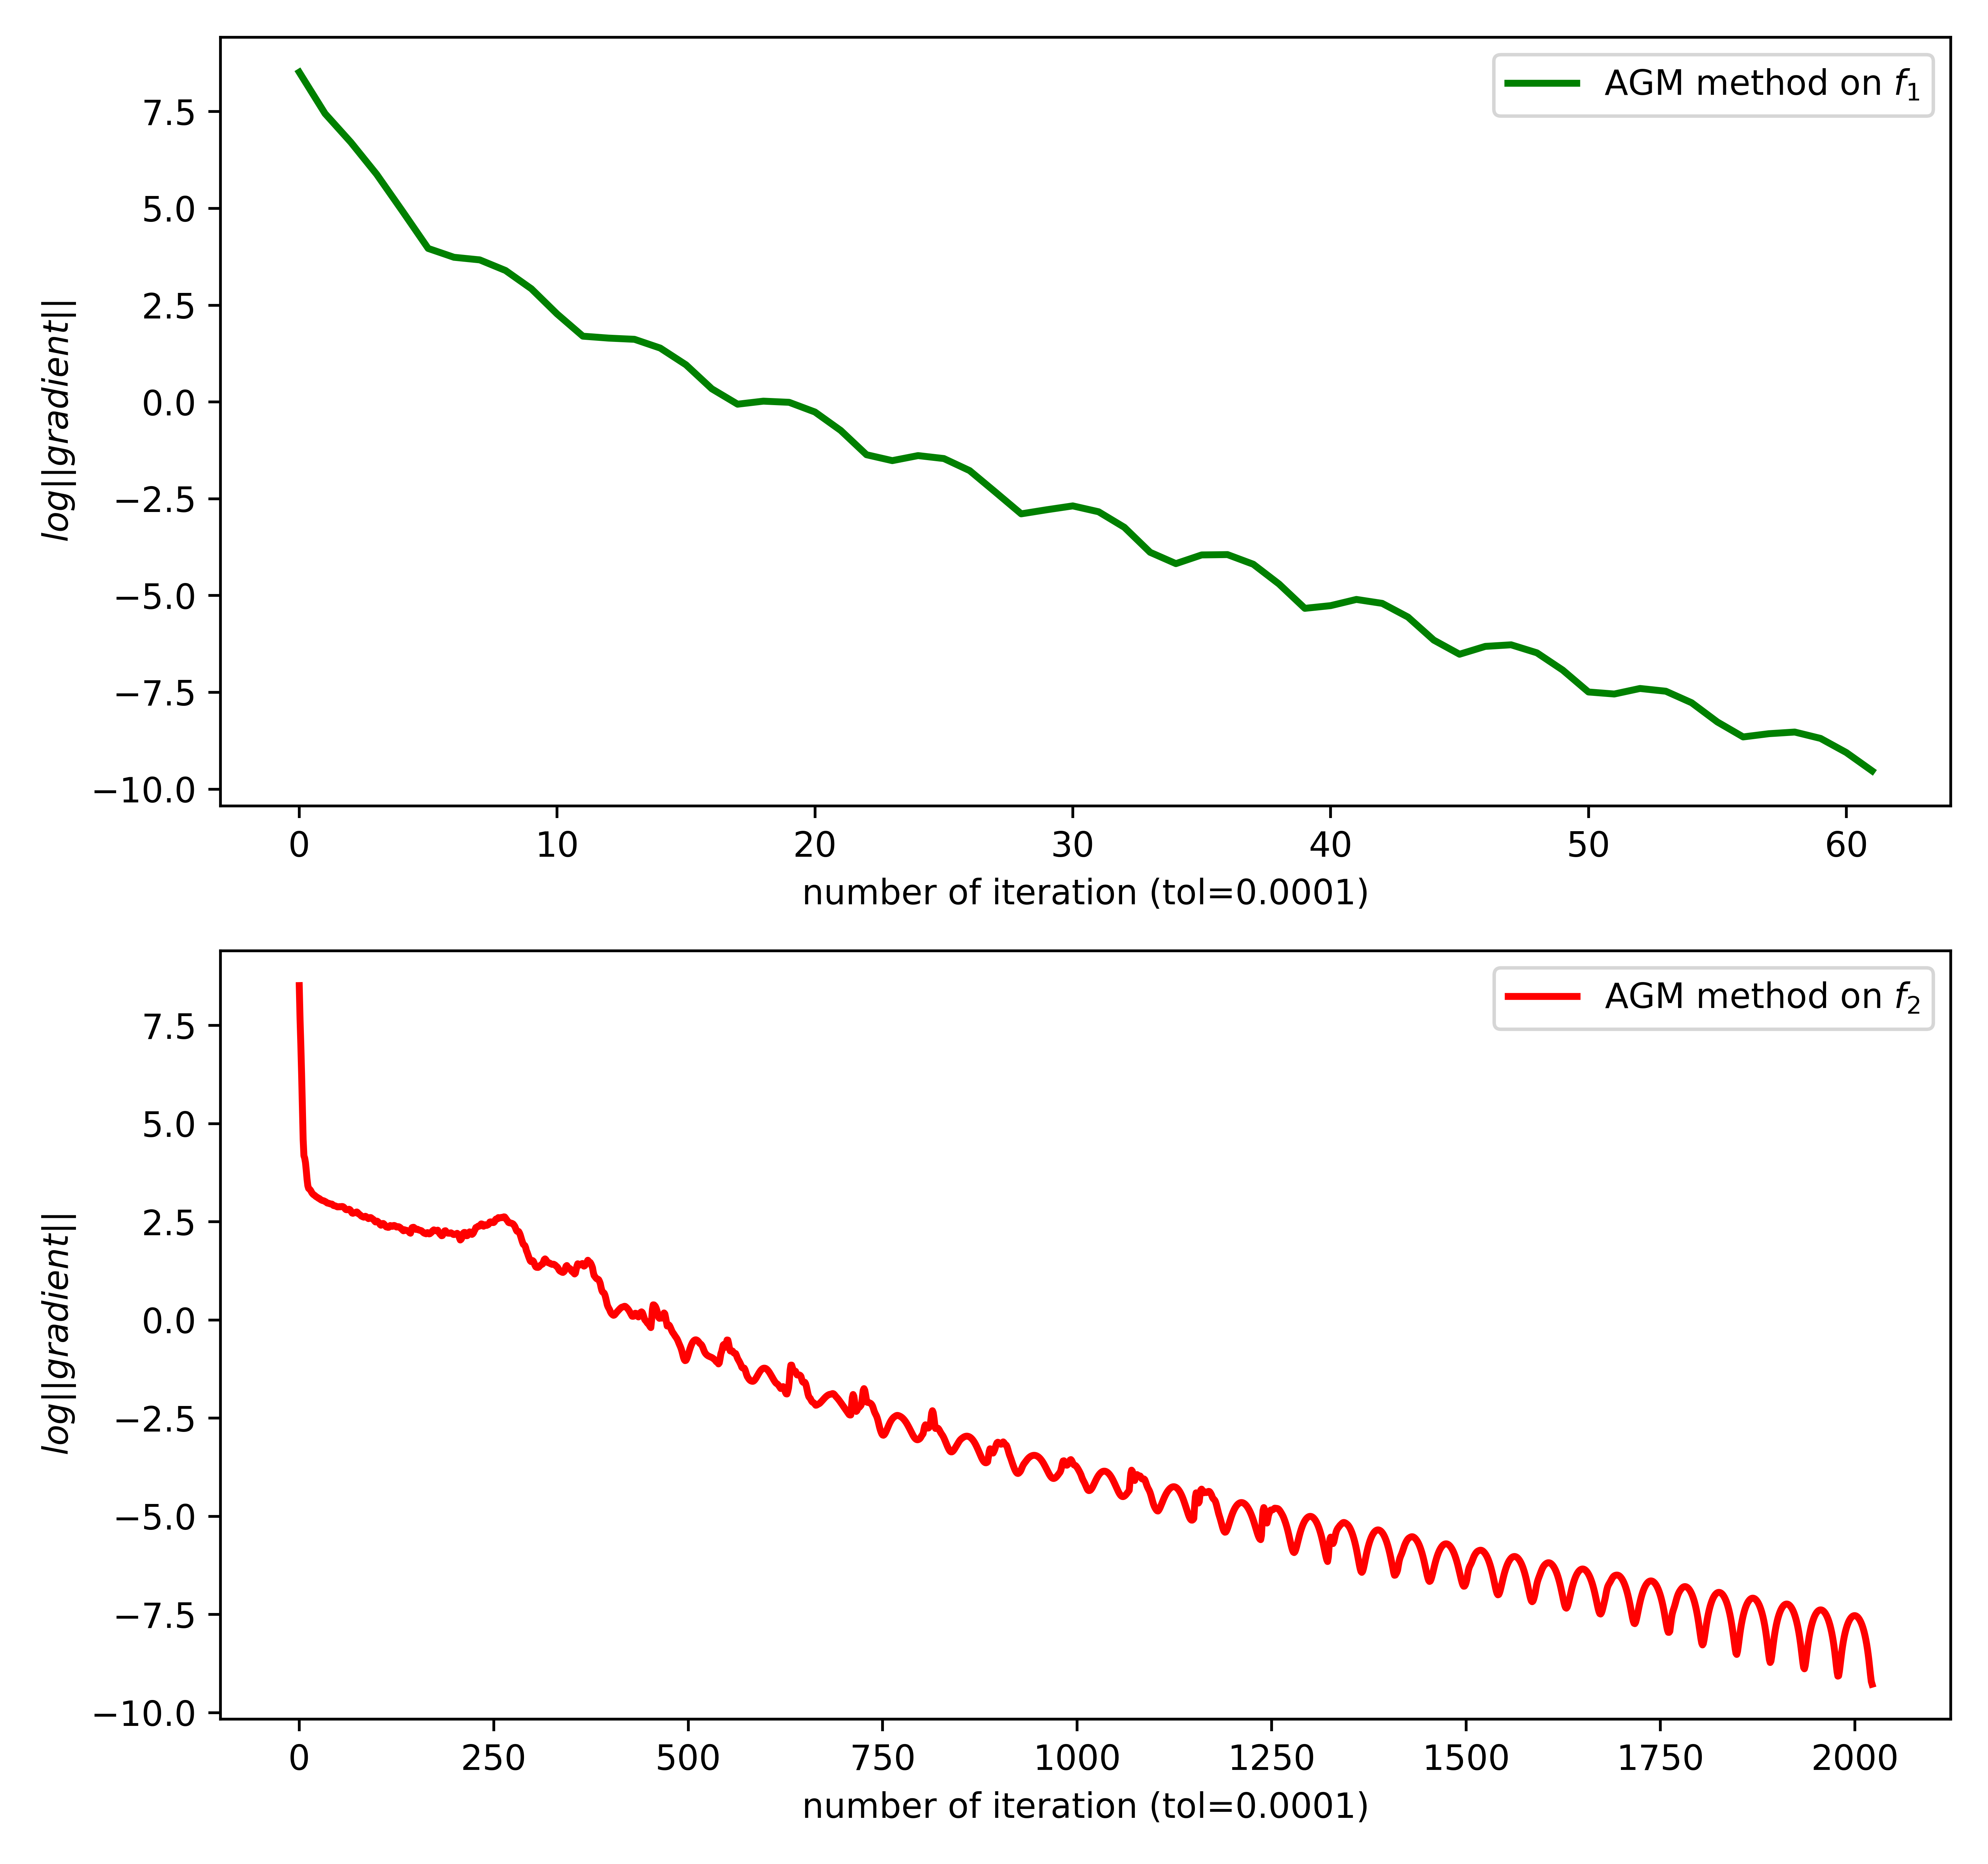
\includegraphics[width=0.5\linewidth]{4_2_a_convergence}
	\vspace{-5pt}
	\caption{The plot of iteration process by AGM}
	\label{AGM1}
\end{figure}

\begin{figure}[htbp]
	\centering
	\subfigure[AGM on $f_1$]{\label{AGMf1}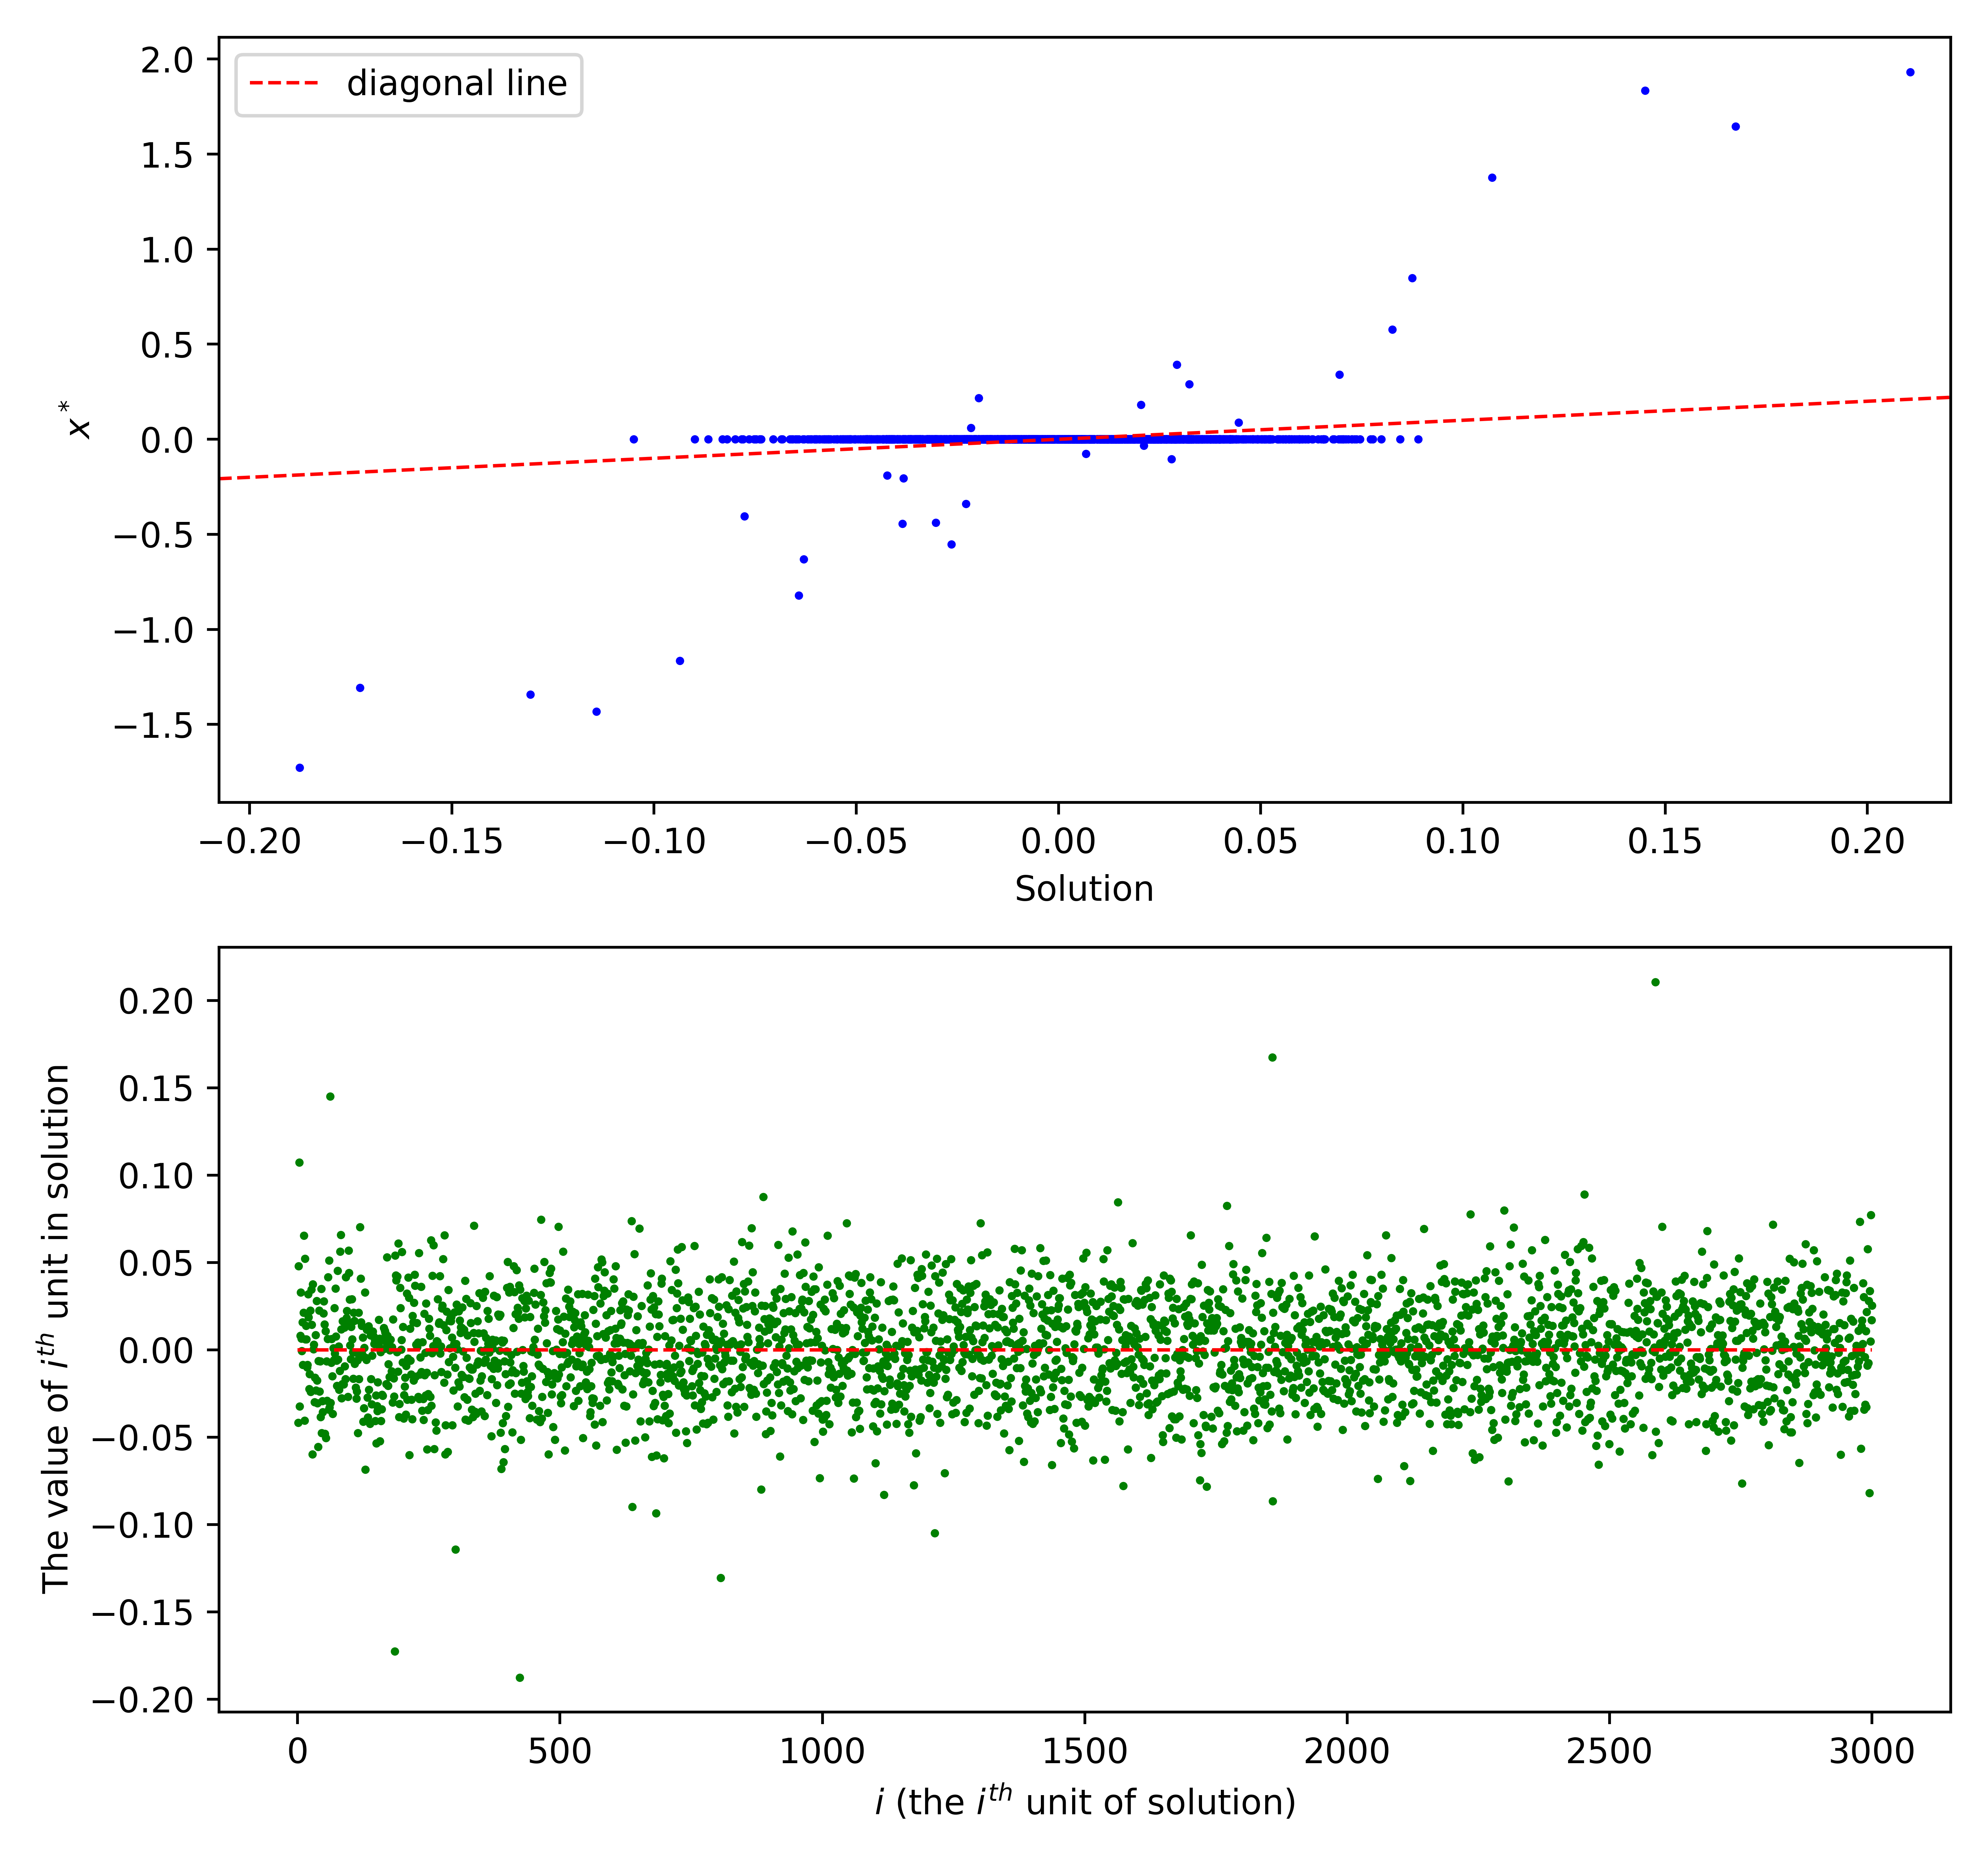
\includegraphics[width=0.4\linewidth]{AGM_compare_f1}}
	\quad
	\subfigure[AGM on $f_2$]{\label{AGMf2}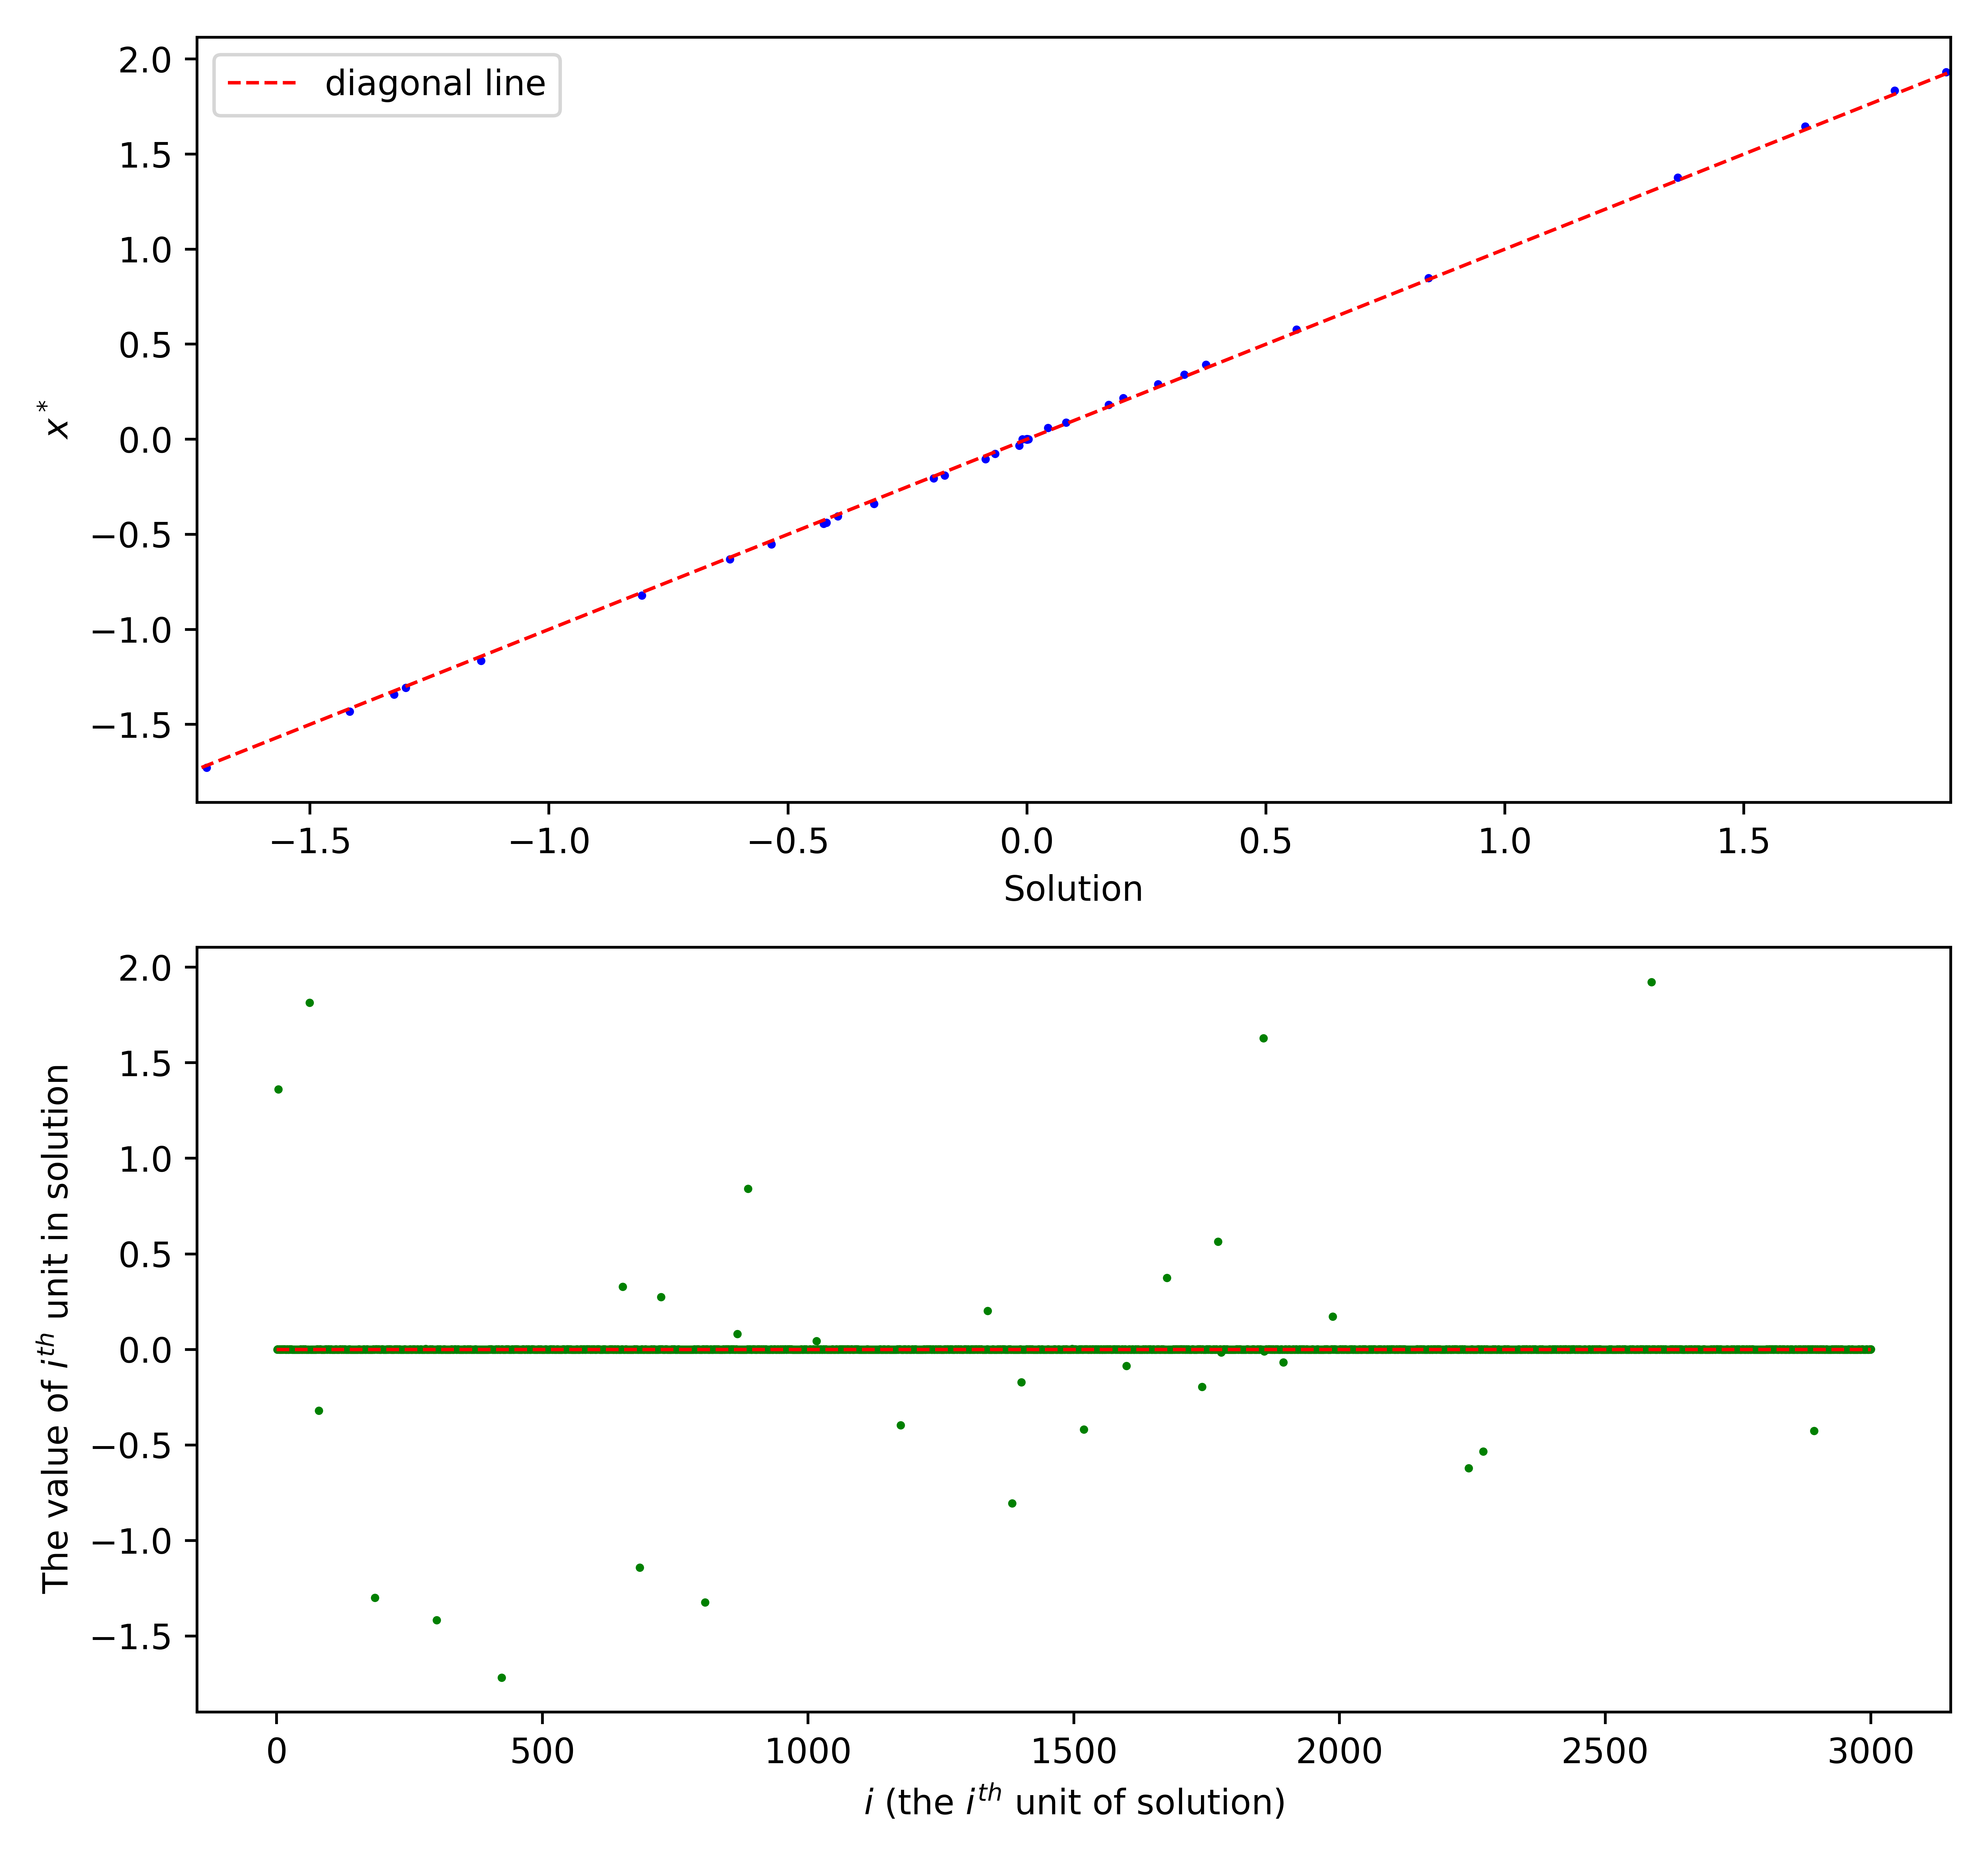
\includegraphics[width=0.4\linewidth]{AGM_compare_f2}}
	\caption{The comparison between solutions and $x^*$, and check the sparse of solutions}
	\label{compare_AGM}
\end{figure}

As we can see from Figure \ref{AGM1}. When we apply AGM to $f_1$, the gradient can converge in 62 times, which is much smaller than that in $f_2$ (2023 times). As we can see from Figure \ref{AGMf1}, When using AGM, $f_1$ is not a good model. This is because the solution is far away from $x^*$, which means the solution is not what we want. Besides, the solution is not sparse, there are small number of 0 in the solution's units actually. On the contrary, as we can see from Figure \ref{AGMf2}, when using AGM, $f_2$ is really a good model. The solution is very close to $x^*$, because they are almost totally on the diagonal line. Besides, the solution is also sparse, there are just small number of units in the solution are not 0, but most units of them are 0, which means the solution is sparse.
\item IGM

For IGM method, we applied it into $f_1$, $f_2$ and $f_3$. We seperated the experiments into two parts: "Know Lipschitz constant" and "Not know Lipschitz constant".
	\begin{enumerate}[$\bullet$ (a):]
		\item Know Lipschitz constant
		\begin{figure}[H]
			\centering
			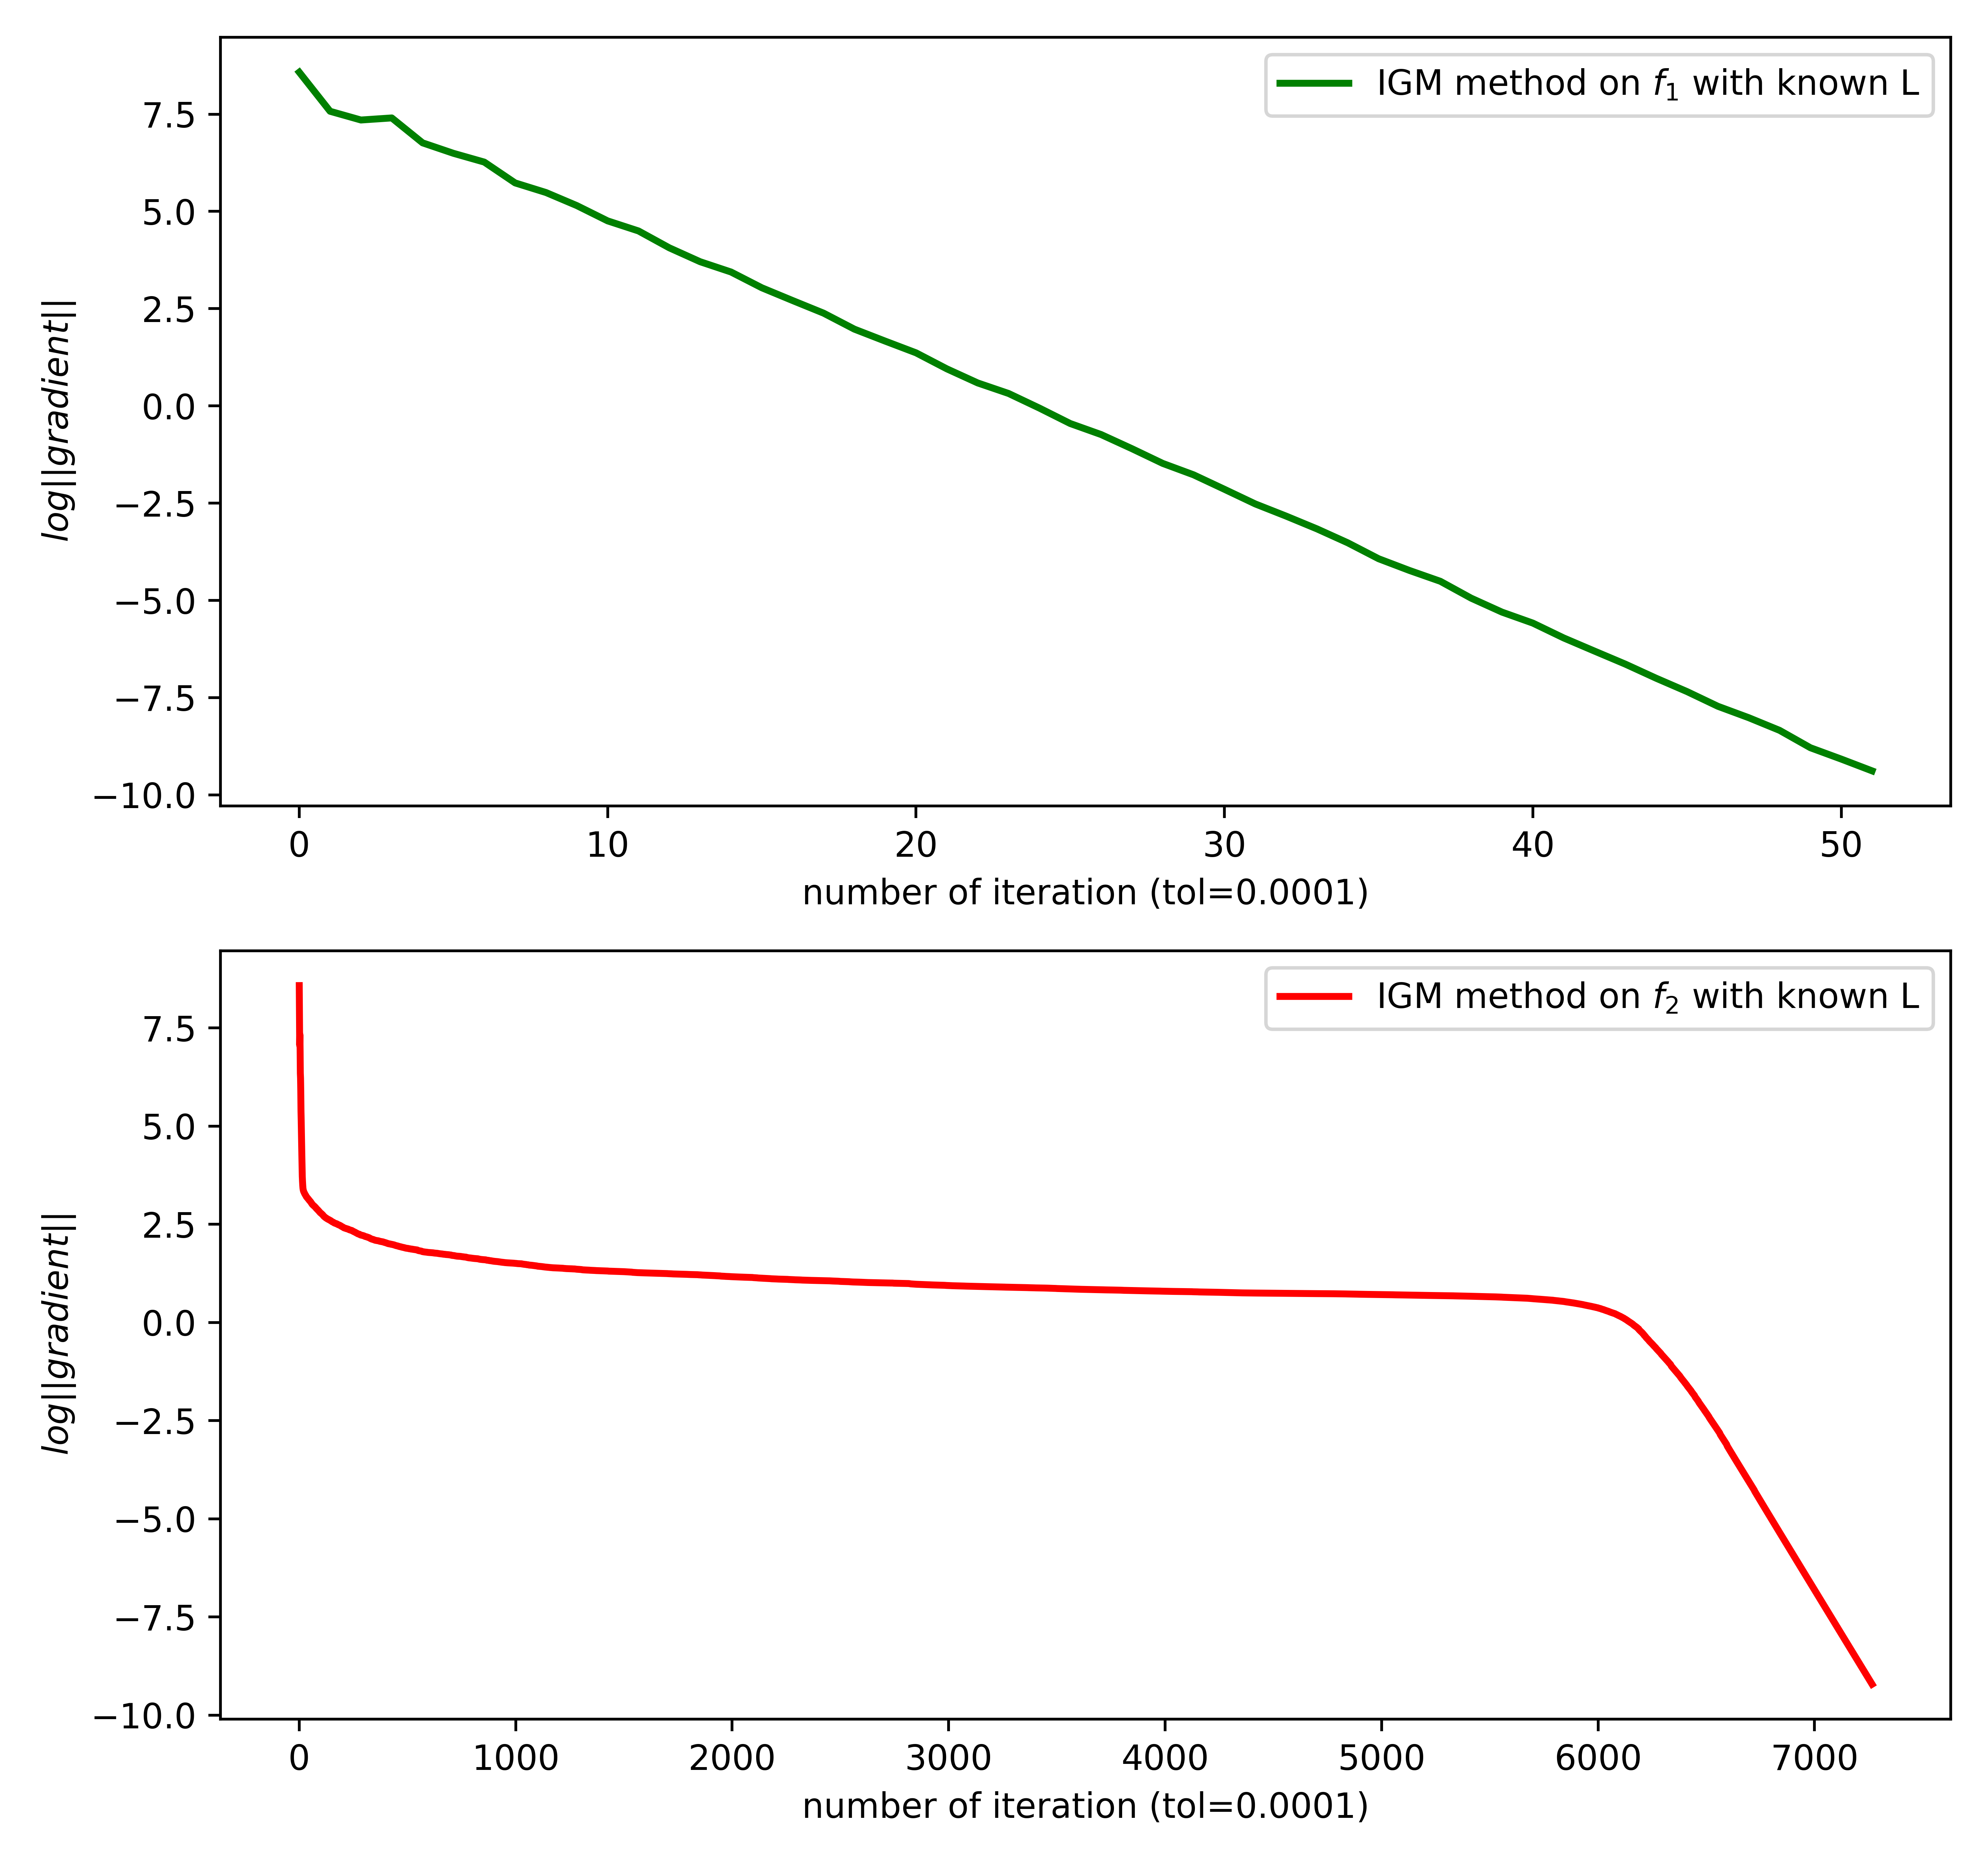
\includegraphics[width=0.5\linewidth]{KnownL}
			\vspace{-5pt}
			\caption{The plot of iteration process by IGM with known $L$}
			\label{IGM1}
		\end{figure}
		
		\begin{figure}[htbp]
			\centering
			\subfigure[IGM on $f_1$ with known $L$]{\label{IGMf1_knwoL}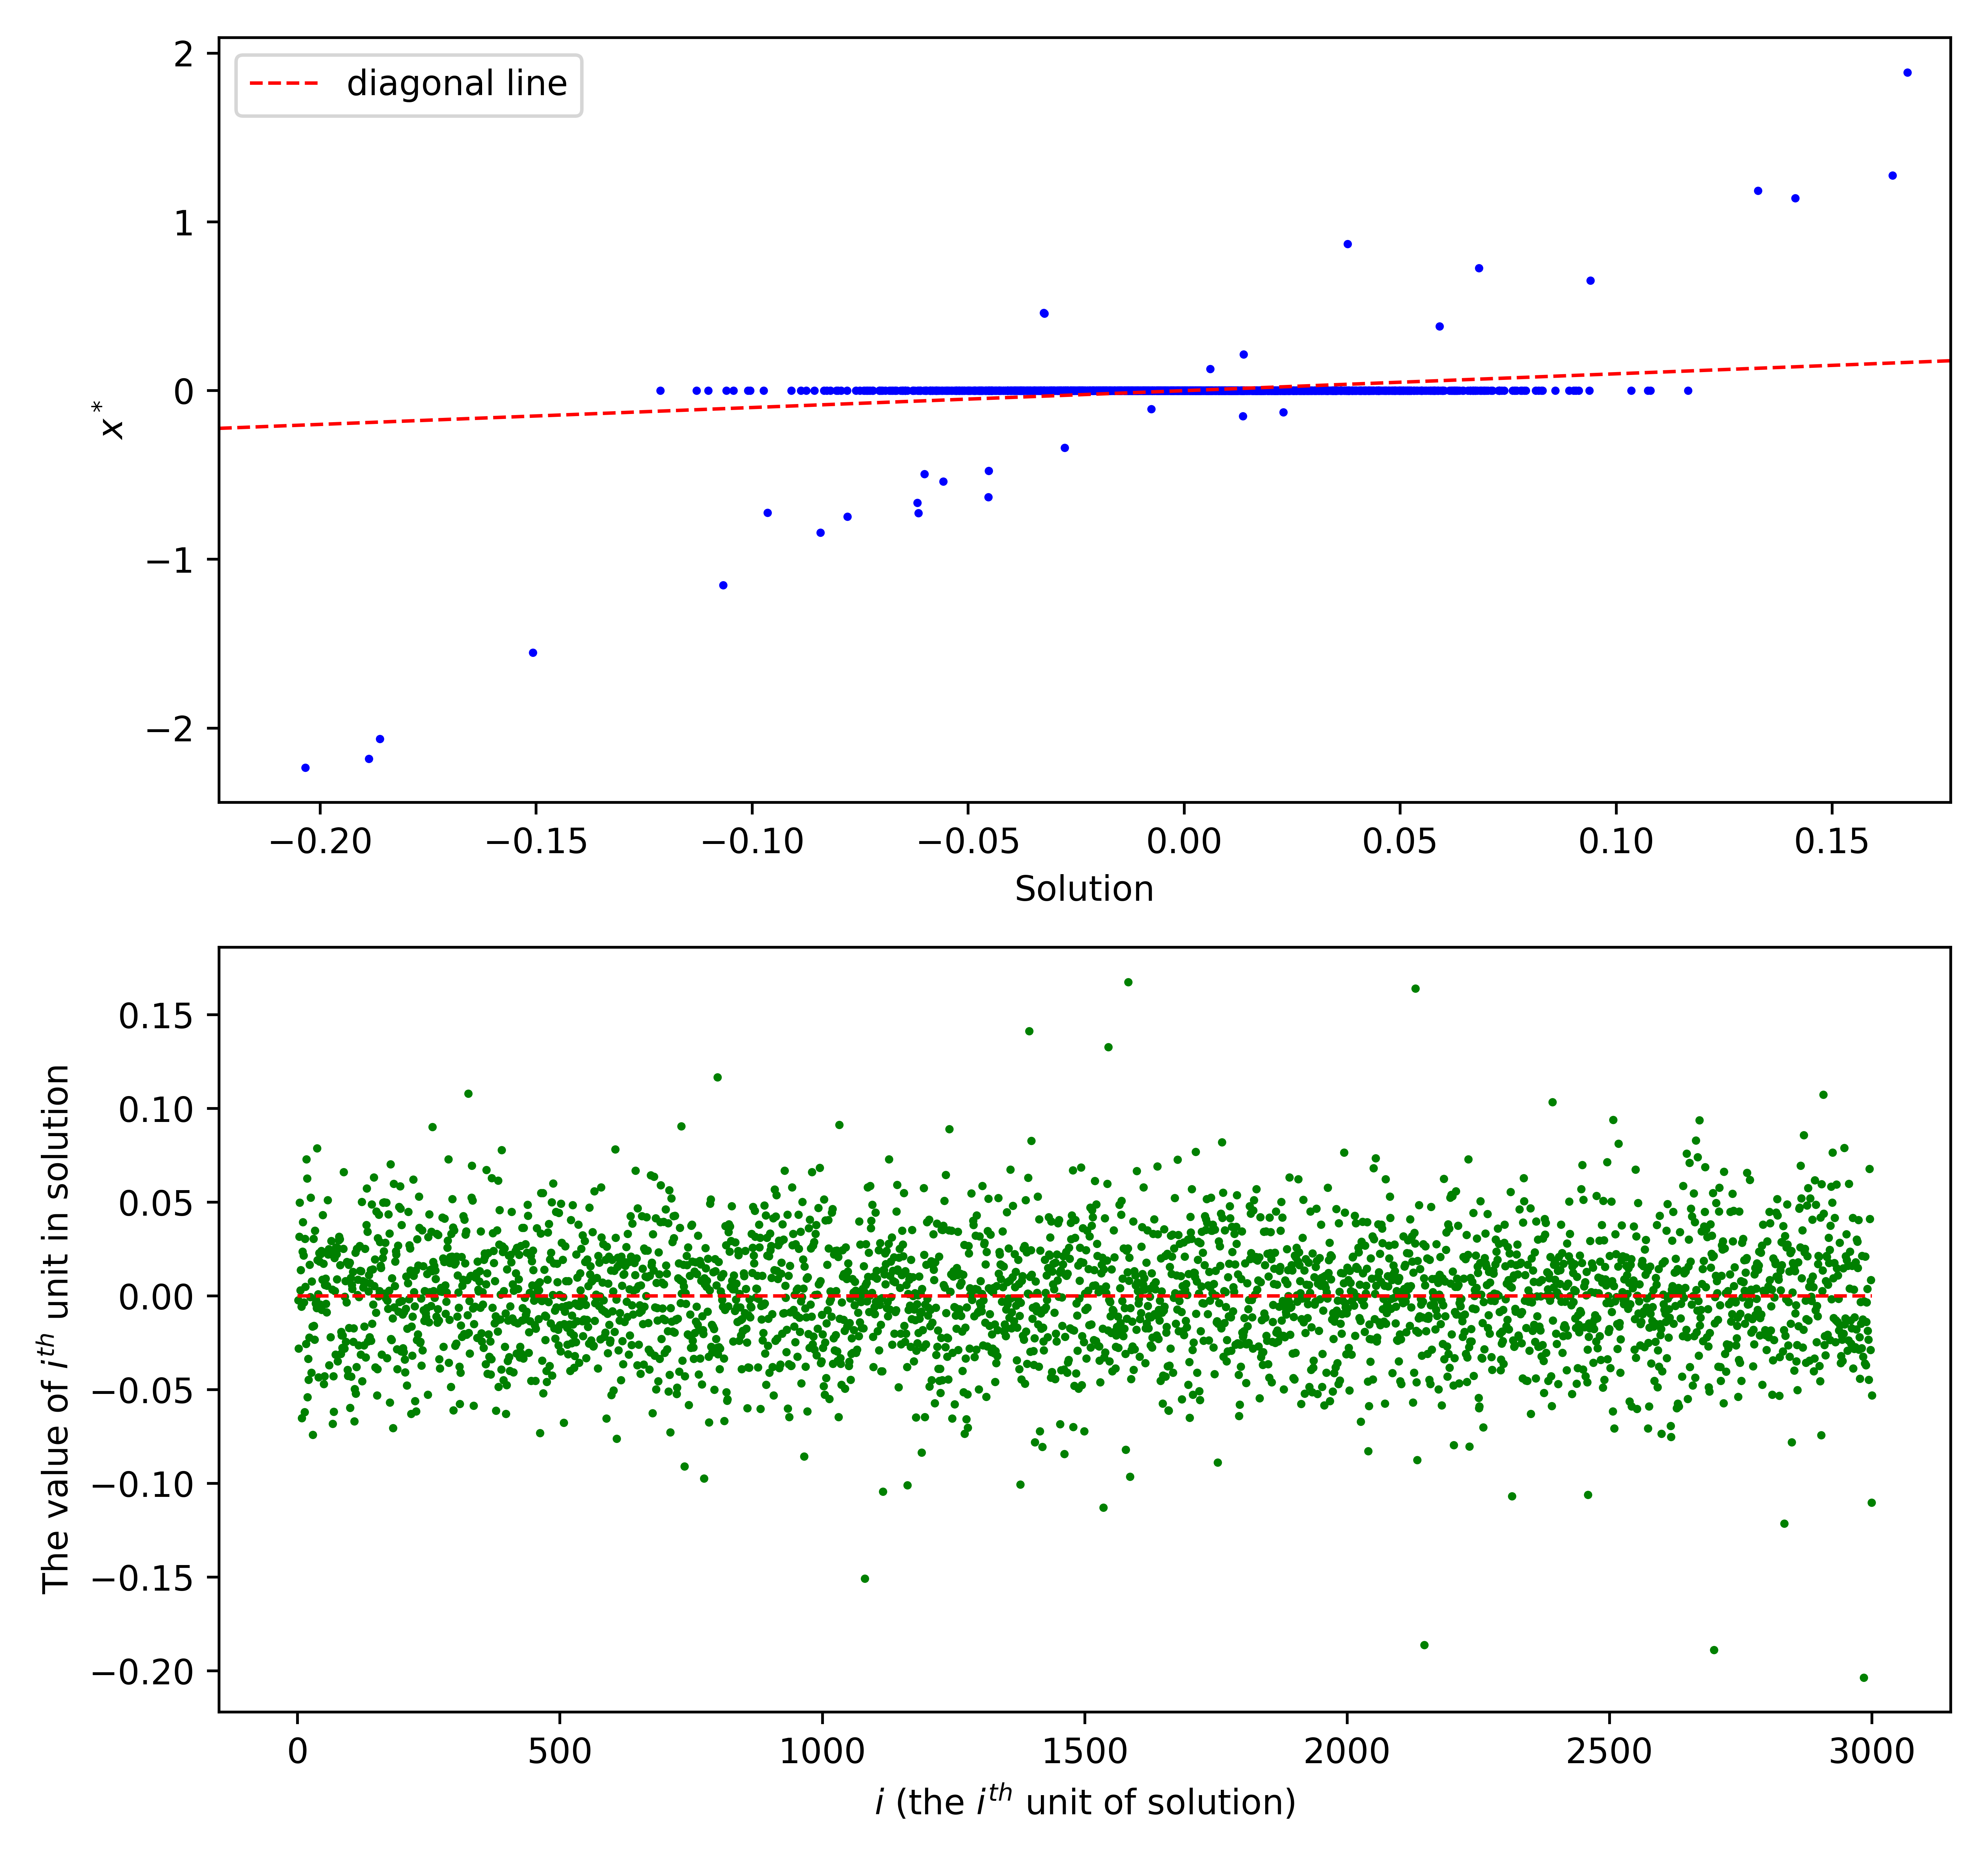
\includegraphics[width=0.47\linewidth]{compare_f1_knwonL}}
			\quad
			\subfigure[IGM on $f_2$ with known $L$]{\label{IGMf2_knowL}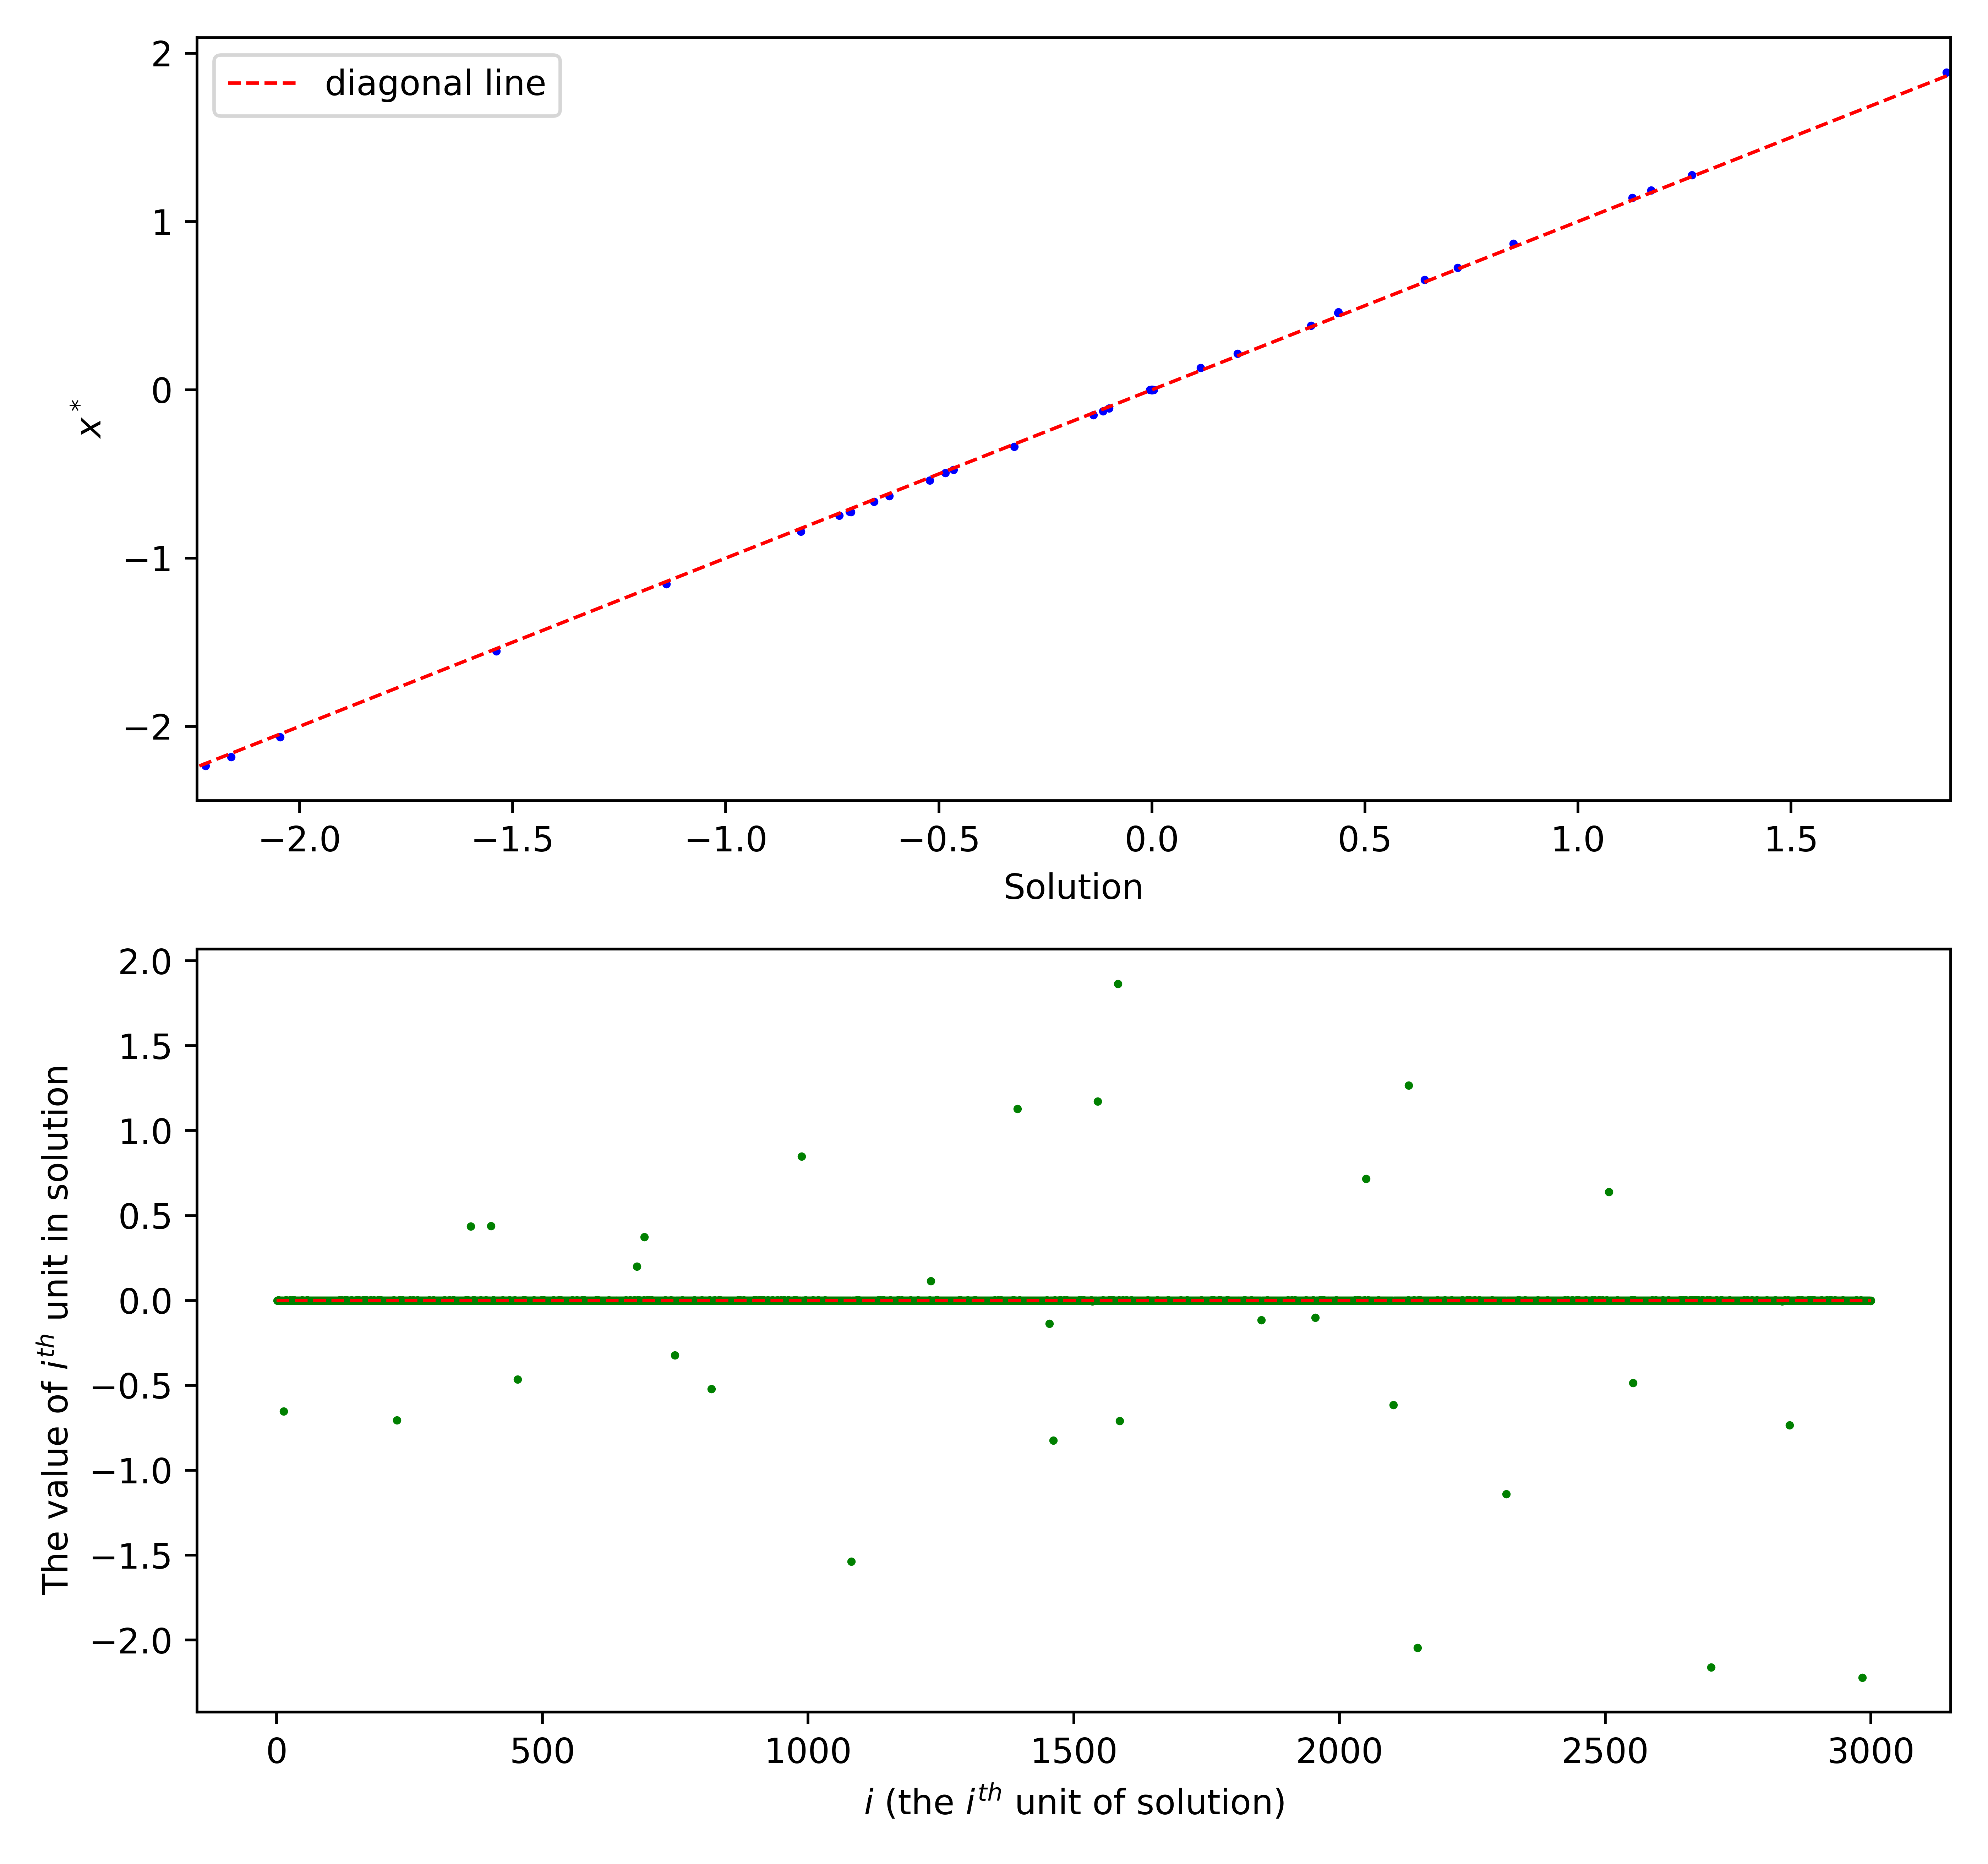
\includegraphics[width=0.47\linewidth]{compare_f2_knwonL}}
			\caption{The comparison between solutions and $x^*$, and check the sparse of solutions)}
			\label{compare_IGMknowL}
		\end{figure}
		
		In this part, we applied IGM into $f_1$ and $f_2$, we computed $L_1$ and $L_2$ explicitly. For $f_1$, we choose the parameters as: $\mu = 1$. For $f_2$, we choose the parameters as: $\mu = 1, \delta = 10^{-3}$. We select $x^0=0$ as the initial point and tol$=10^{-4}$. The performance is measured by comparing $\|\nabla f(x^k)\|$. The result is showed in Figure \ref{IGM1}. Then, we reconstruct solution and compate them with $x^*$, the result is showed as Figure \ref{compare_IGMknowL}.
		
		As we can see from Figure \ref{IGM1}, when we apply IGM with known $L$ to $f_1$, the gradient can converge in 52 times, which is much smaller than that in $f_2$ (7267 times). And we can see that there is a plateau period in the convergence process of the gradient of $f_2$. 
		
		As we can see from Figure \ref{IGMf1_knwoL}, When using IGM with known $L$, $f_1$ is not a good model. This is because the solution is far away from $x^*$, which means the solution is not what we want. Besides, the solution is not sparse, there are small number of 0 in the solution's units actually. On the contrary, as we can see from Figure \ref{IGMf2_knowL}, when using IGM with known $L$, $f_2$ is really a good model. The solution is very close to $x^*$, because they are almost totally on the diagonal line. Besides, the solution is also sparse, there are just small number of units in the solution are not 0, but most units of them are 0, which means the solution is sparse.
		
		\item Not know Lipschitz constant
		
		In this part, we applied IGM into $f_1$, $f_2$ and $f_3$, we do not compute $L_1$, $L_2$ and $L_3$ explicitly. On the contrary, we treat the Lipschitz constant as unknown, and we use Algorithm 1 (mentioned before) as a variant to do IGM. For $f_1$, we choose the parameters as: $\mu = 1$. For $f_2$, we choose the parameters as: $\mu = 1, \delta = 10^{-3}$. For $f_3$, we choose the parameters as: $\mu = 1, \delta = 10^{-3}, \nu=10^{-4}$.We select $x^0=0$ as the initial point and tol$=10^{-4}$. The performance is measured by comparing $\|\nabla f(x^k)\|$. The result is showed in Figure \ref{IGM2}. Then, we reconstruct solution and compate them with $x^*$, the result is showed as Figure \ref{compare_IGMunknownL}. 
		\begin{figure}[H]
			\centering
			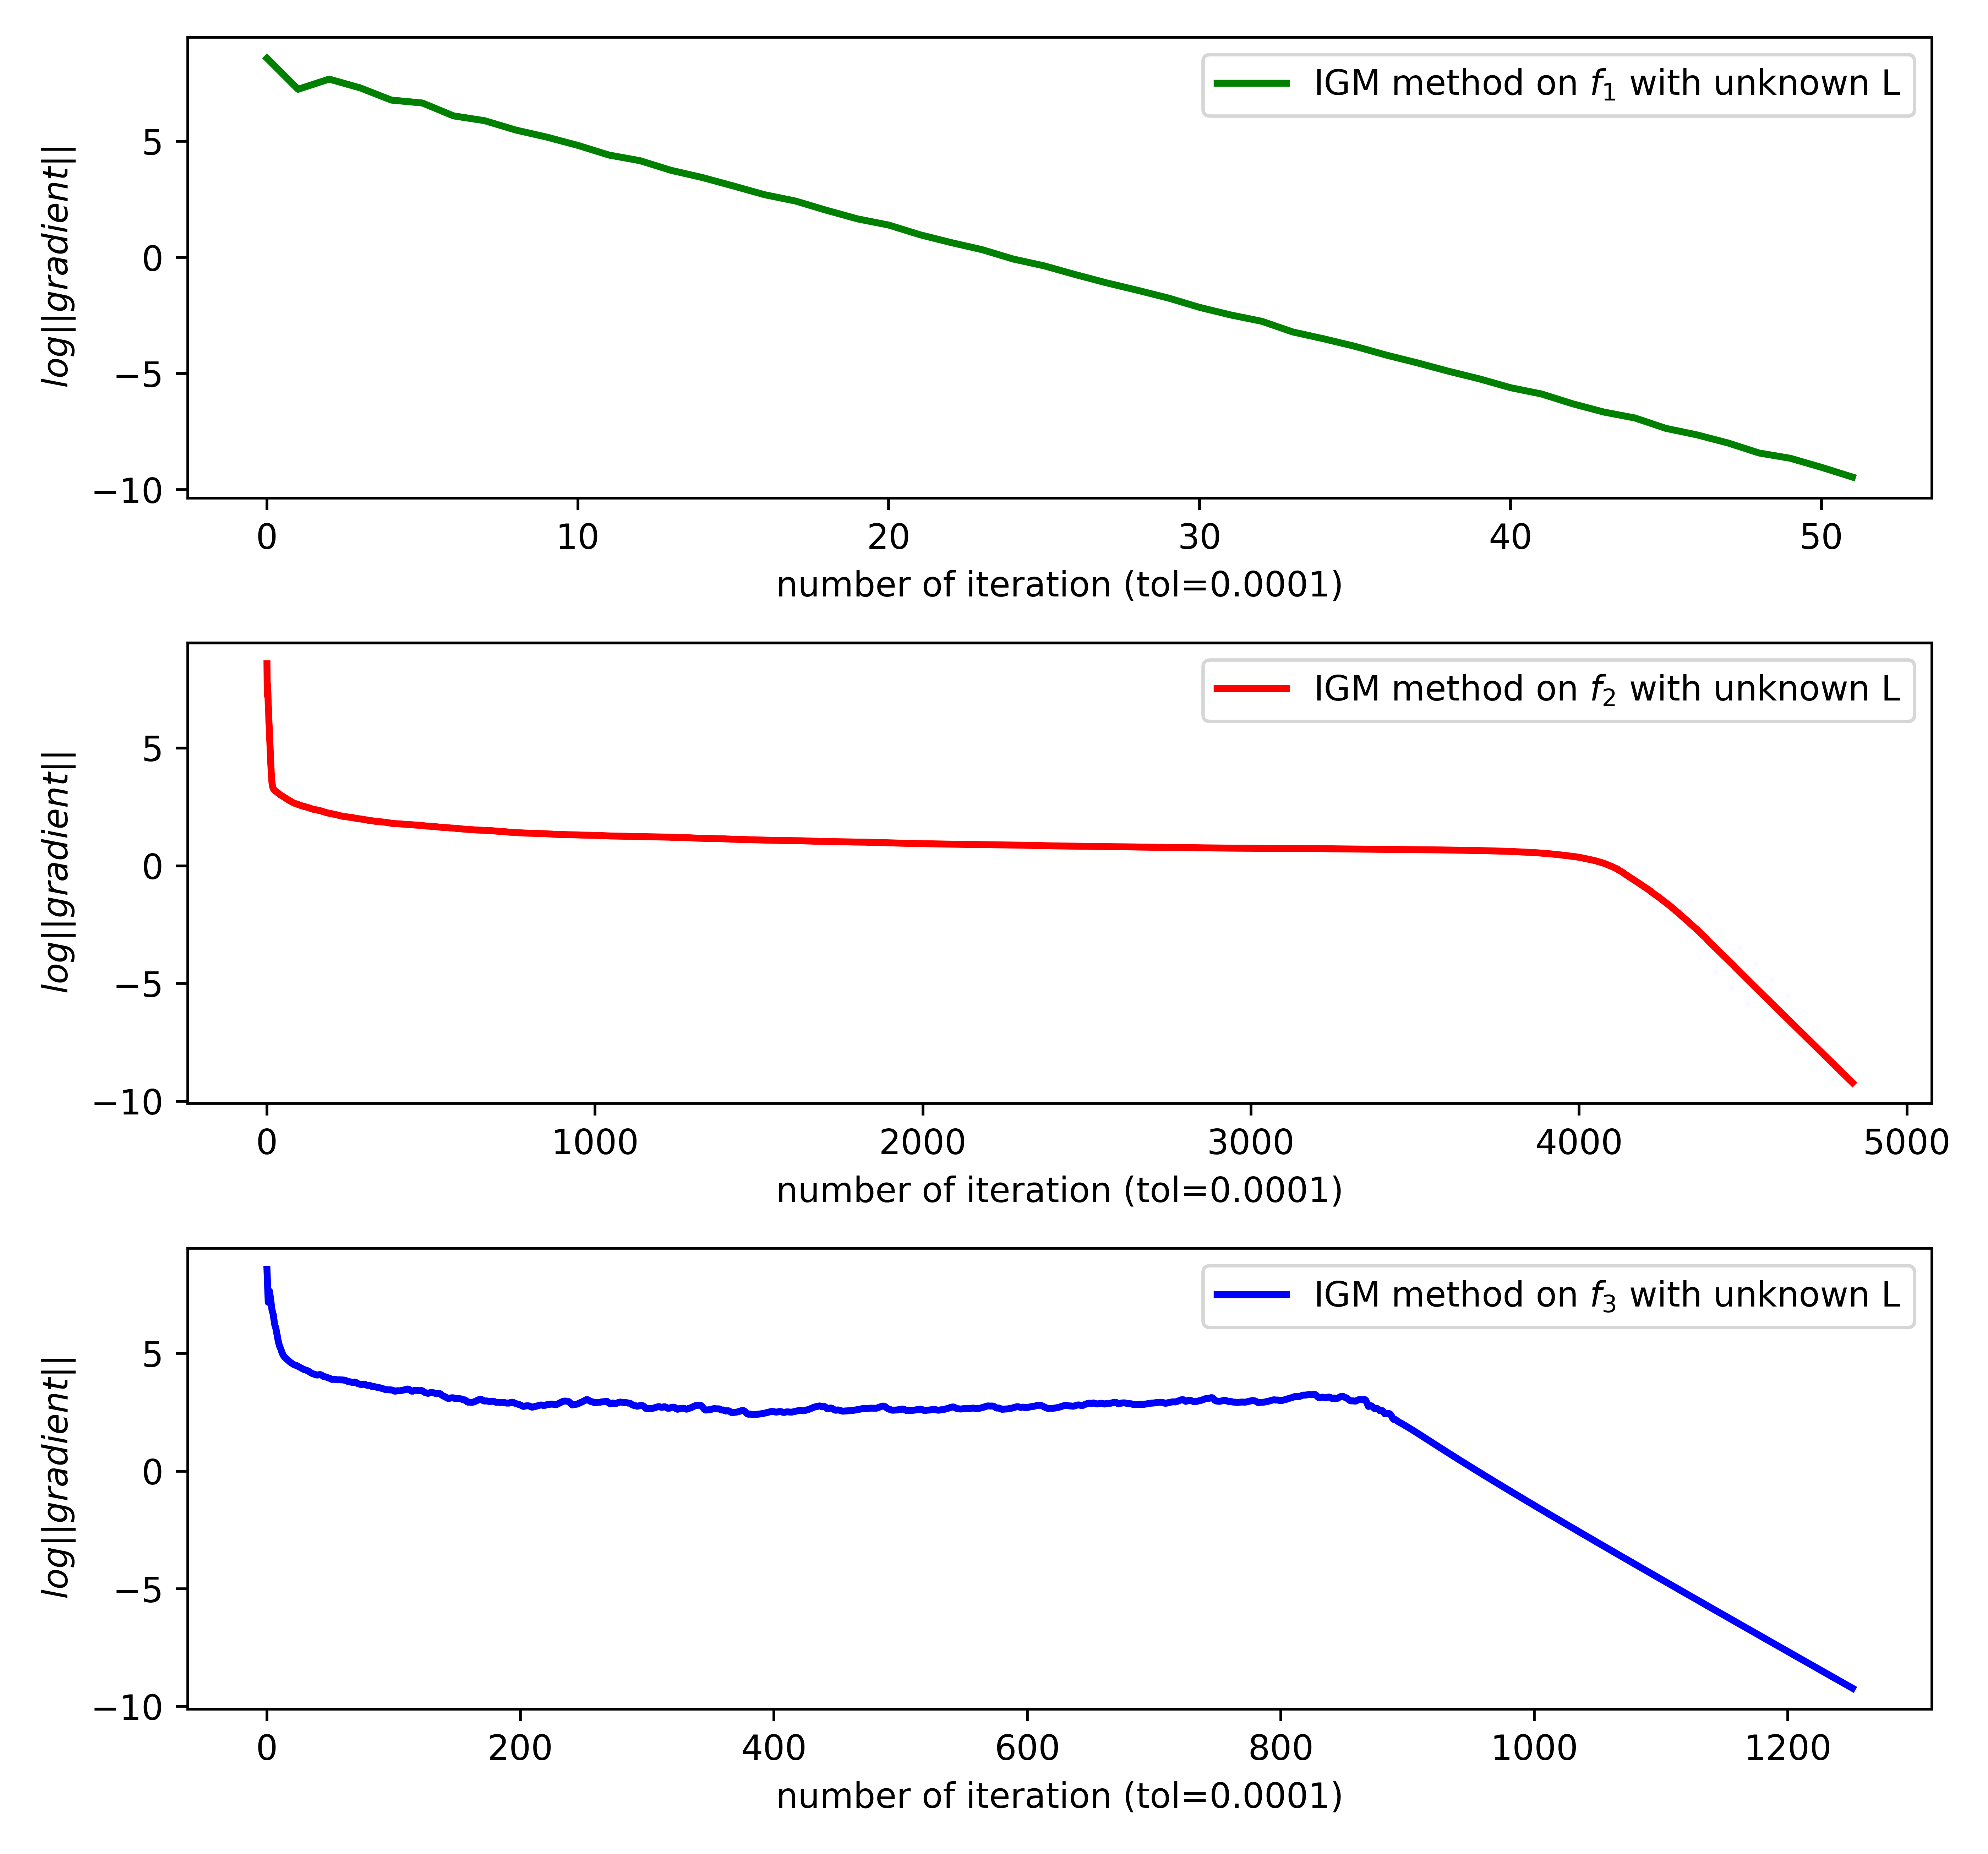
\includegraphics[width=0.55\linewidth]{UnknownL}
			\vspace{-5pt}
			\caption{The plot of iteration process by IGM with unknown $L$}
			\label{IGM2}
		\end{figure}
		
		
		\begin{figure}[htbp]
			\centering
			\subfigure[IGM on $f_1$ with unknown $L$]{\label{IGMf1_unknownL}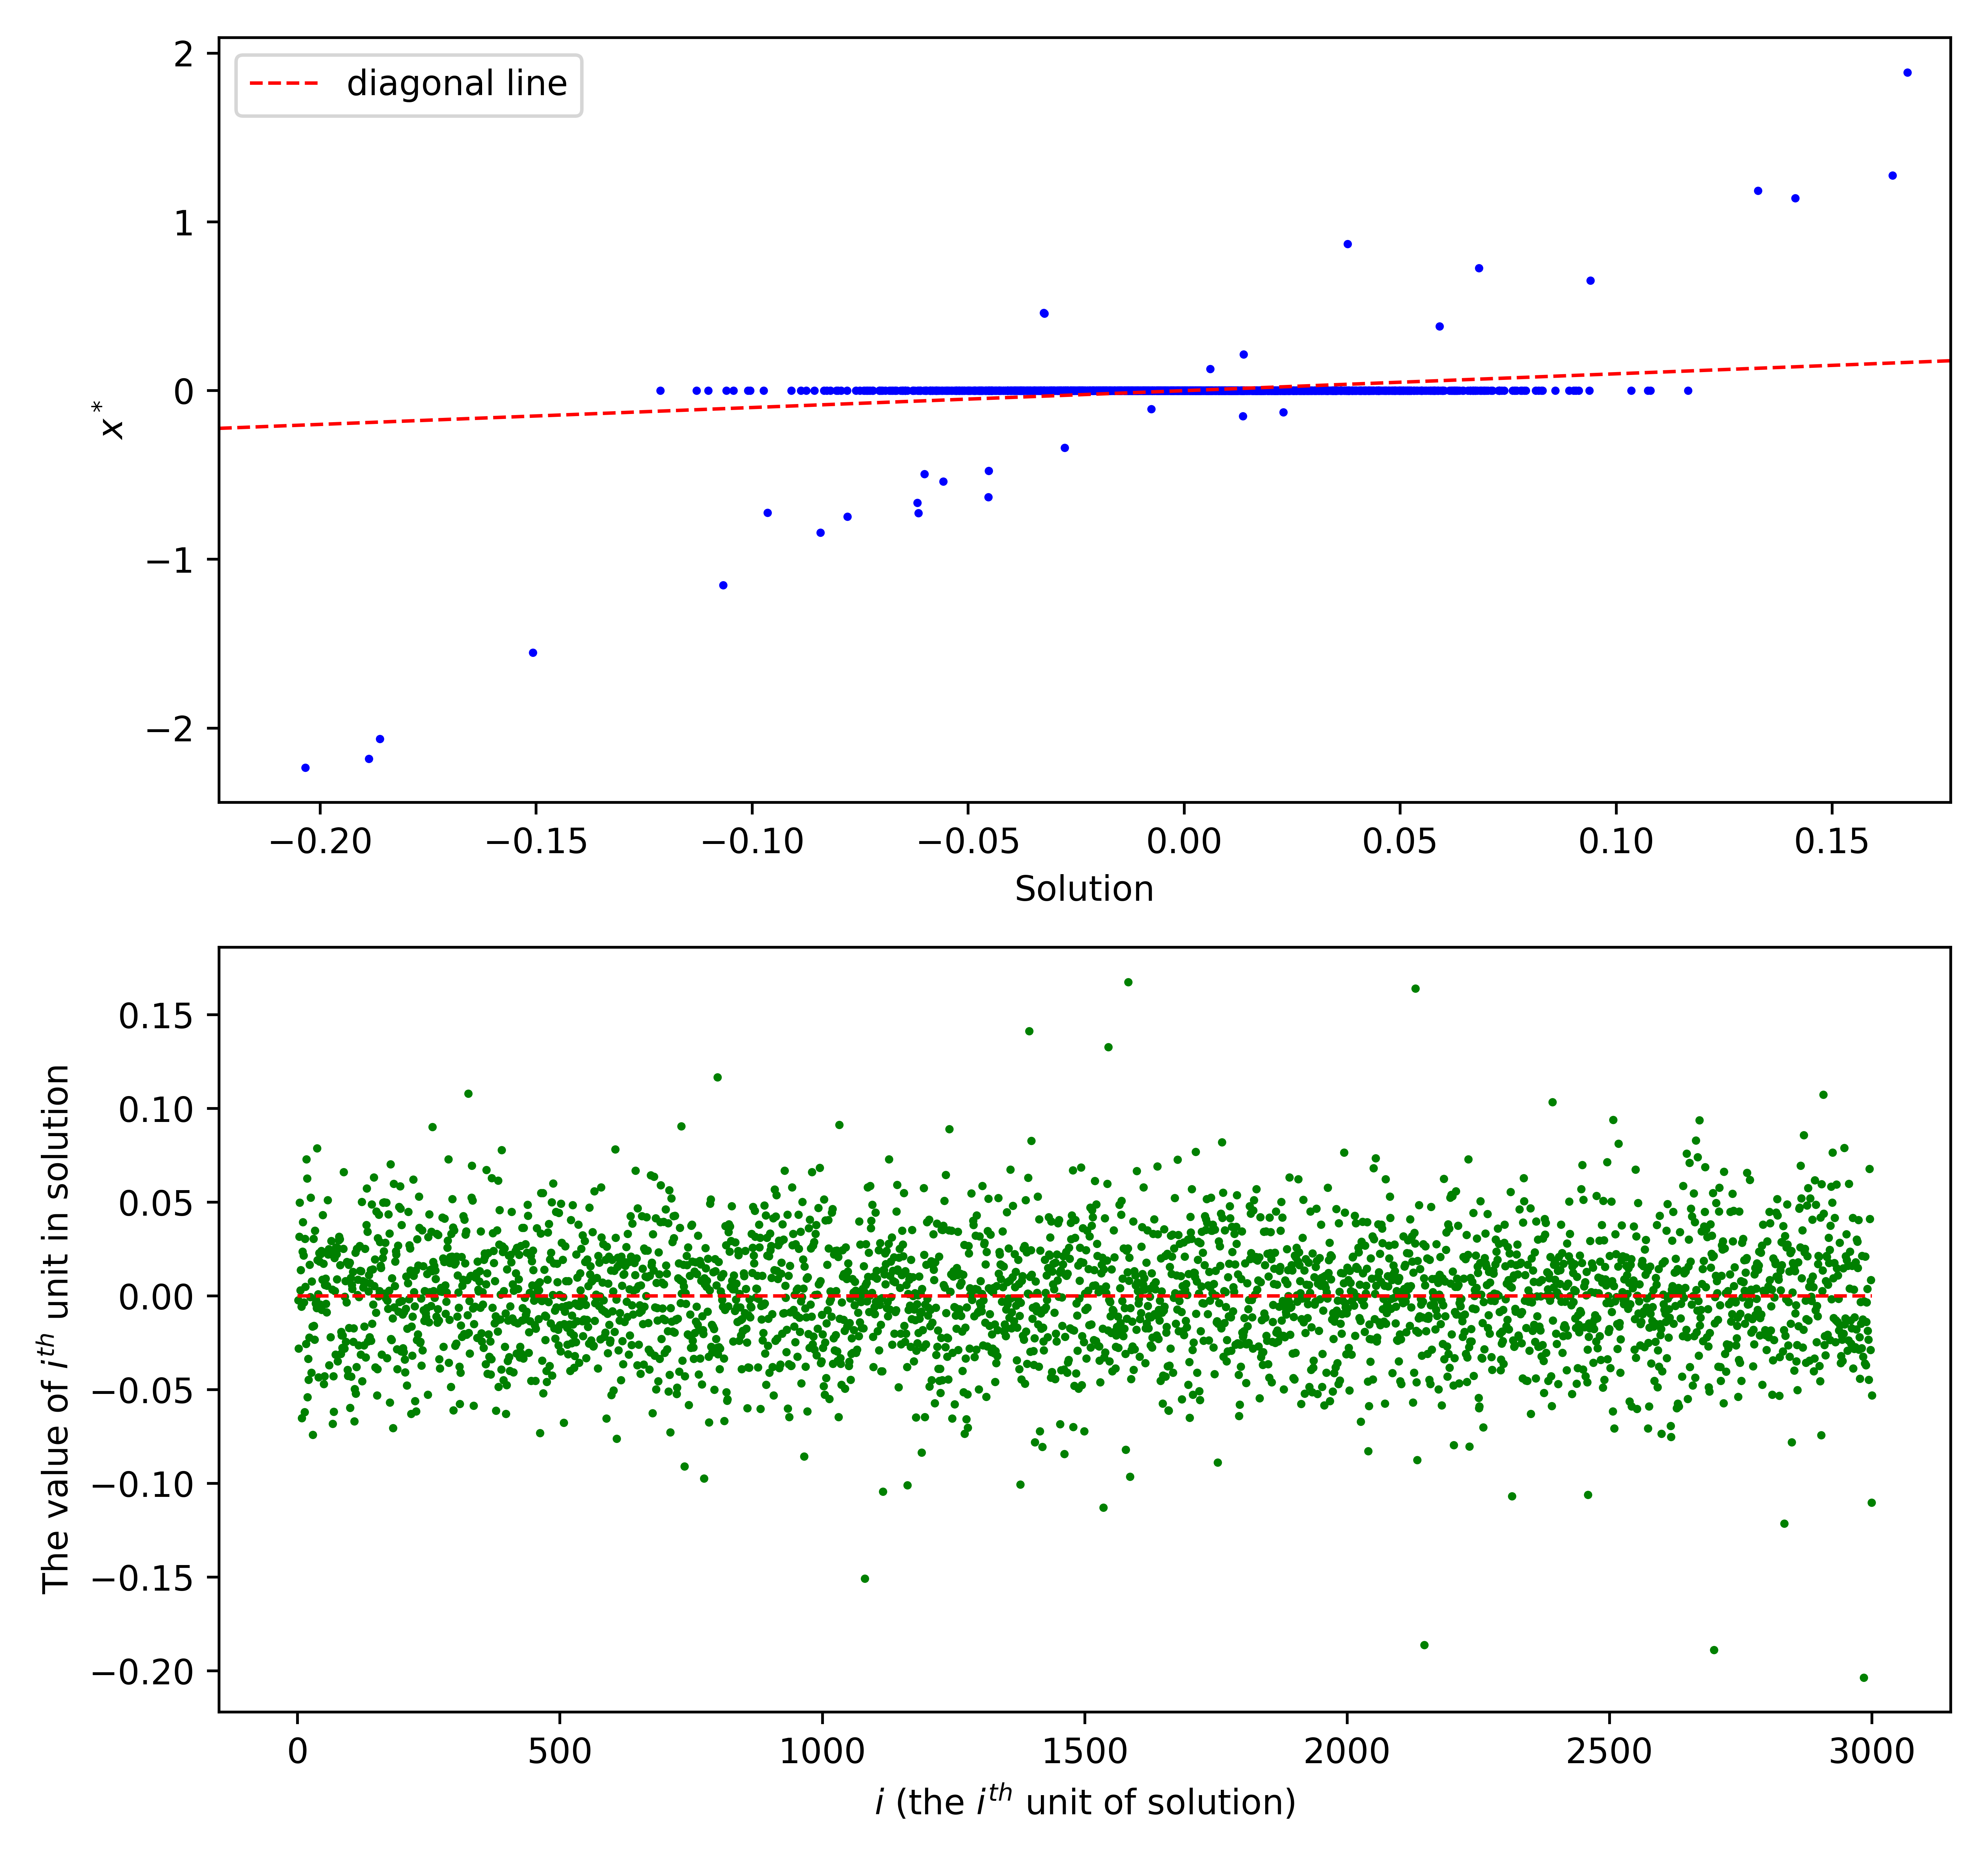
\includegraphics[width=0.3\linewidth]{compare_f1_UnknownL}}
			\quad
			\subfigure[IGM on $f_2$ with unknown $L$]{\label{IGMf2_unknownL}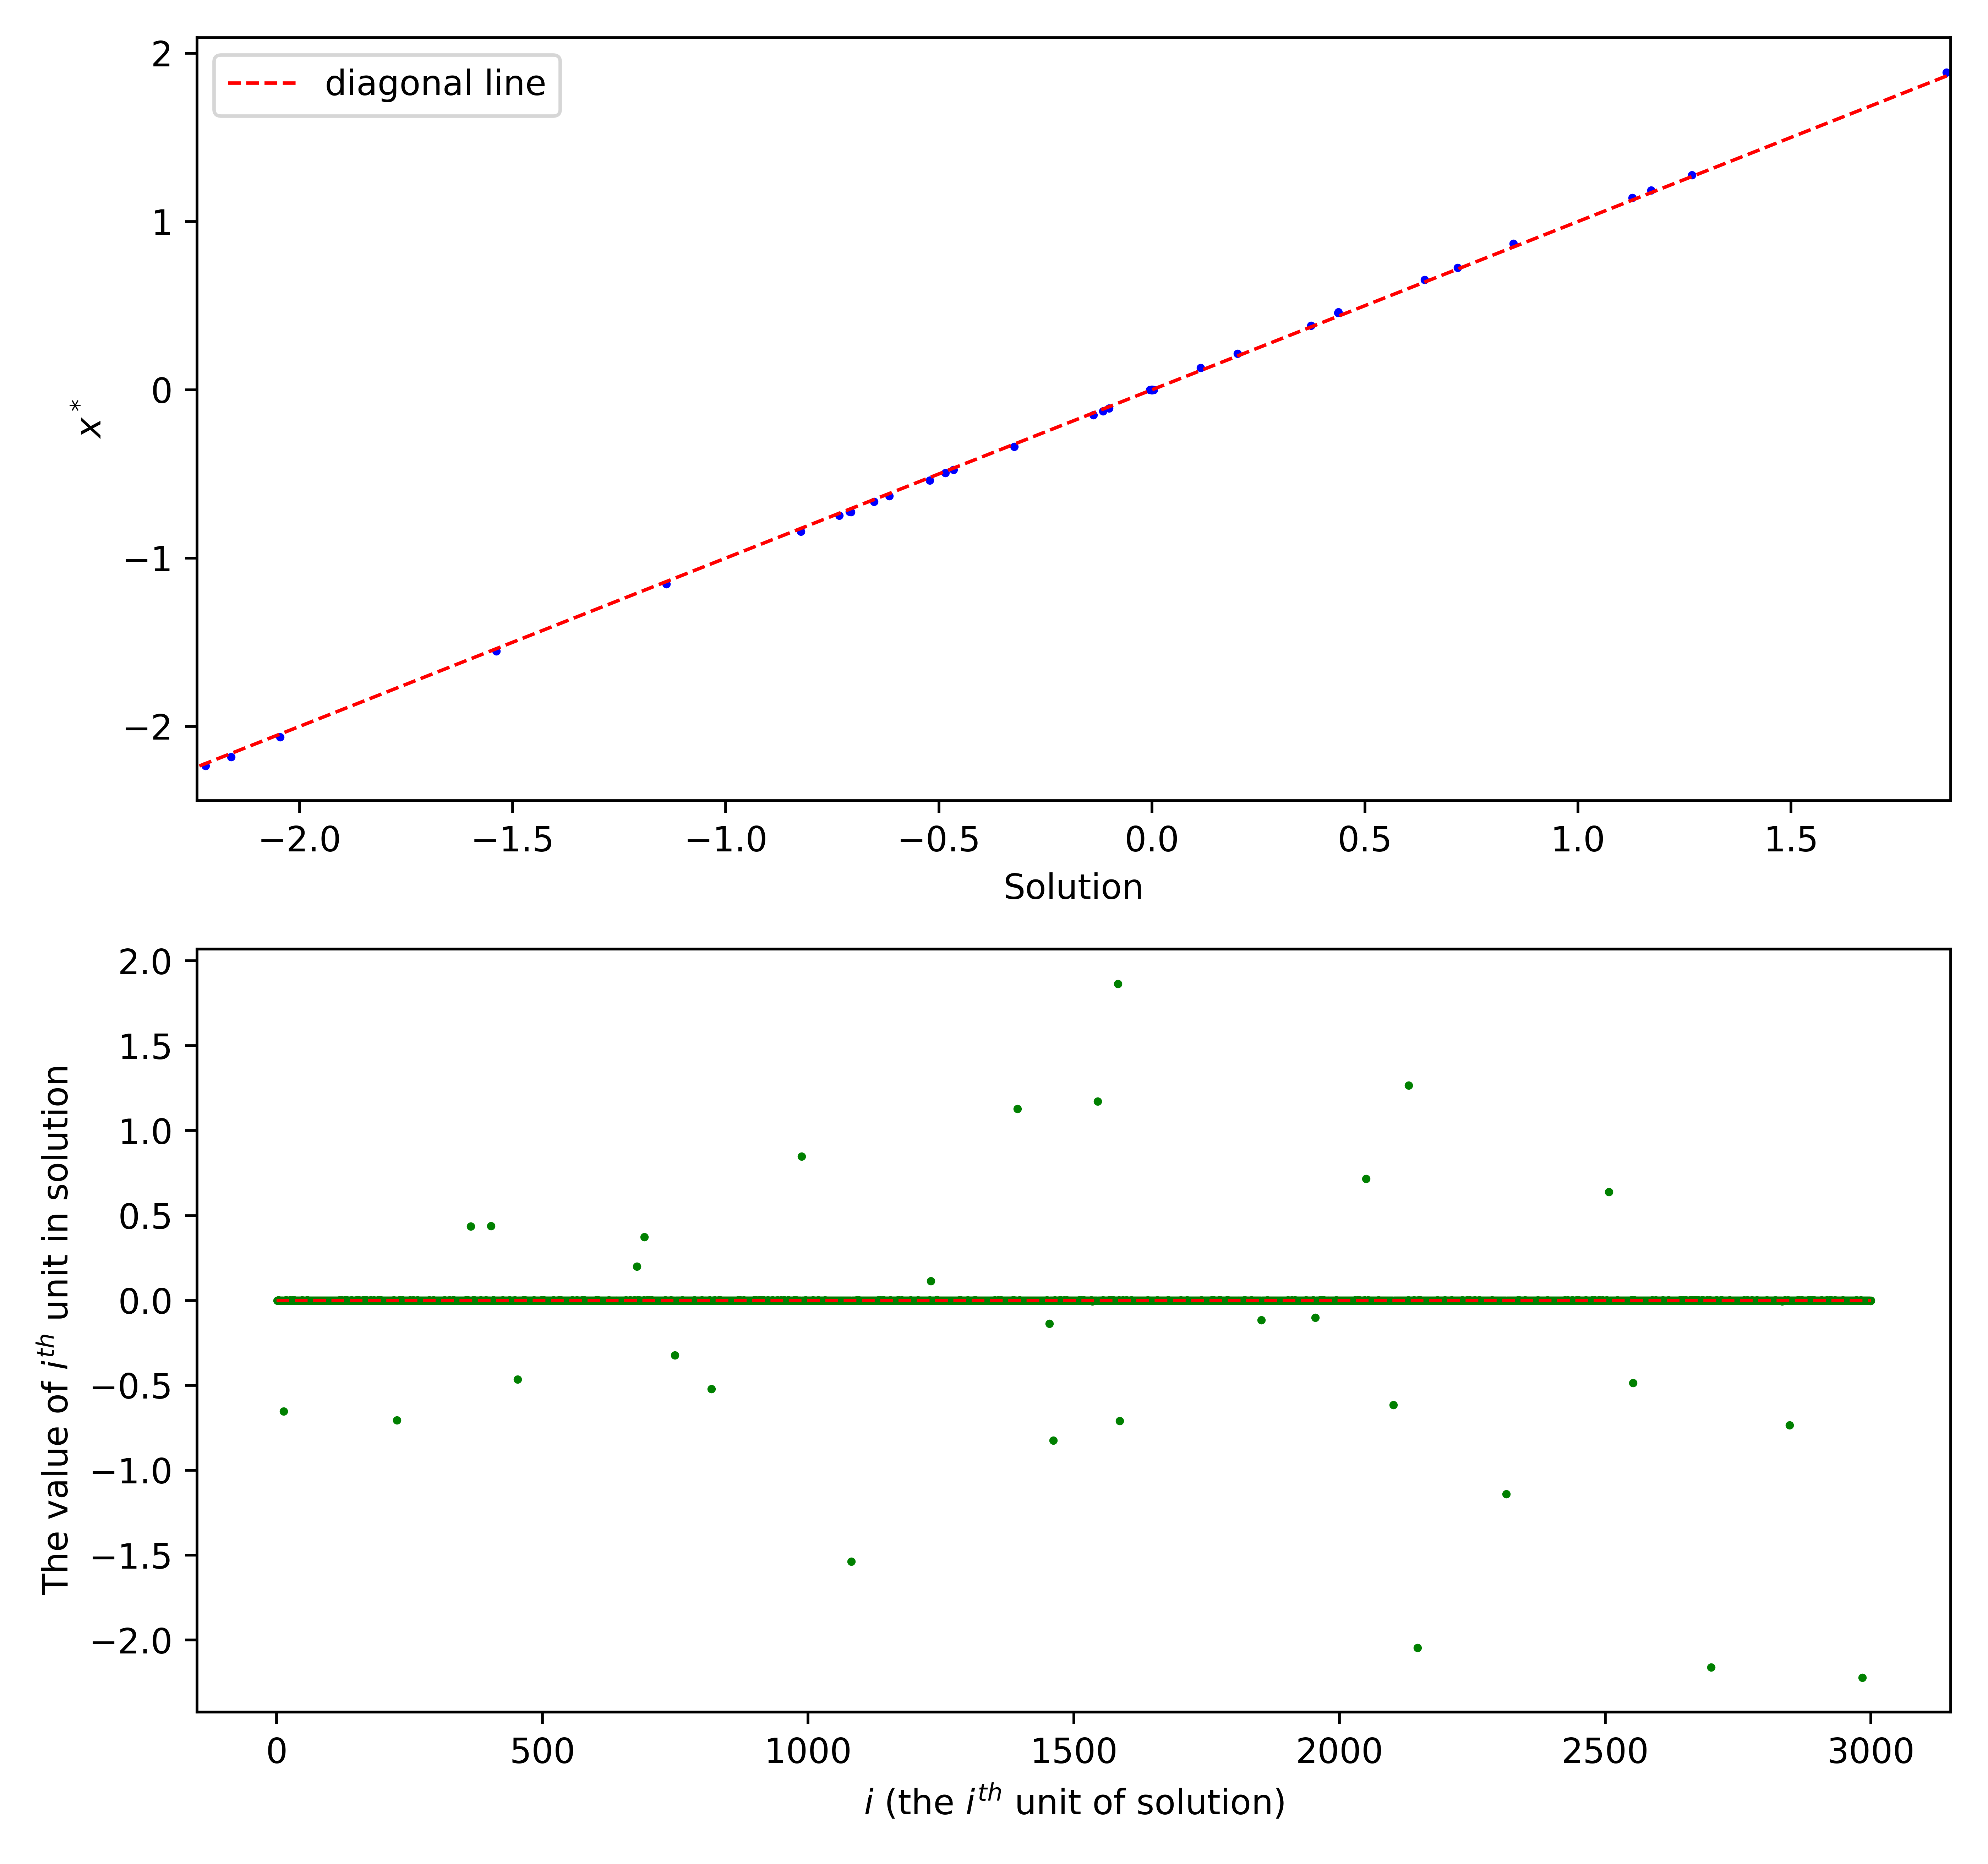
\includegraphics[width=0.3\linewidth]{compare_f2_UnknownL}}
			\quad
			\subfigure[IGM on $f_3$ with unknown $L$]{\label{IGMf3_unknownL}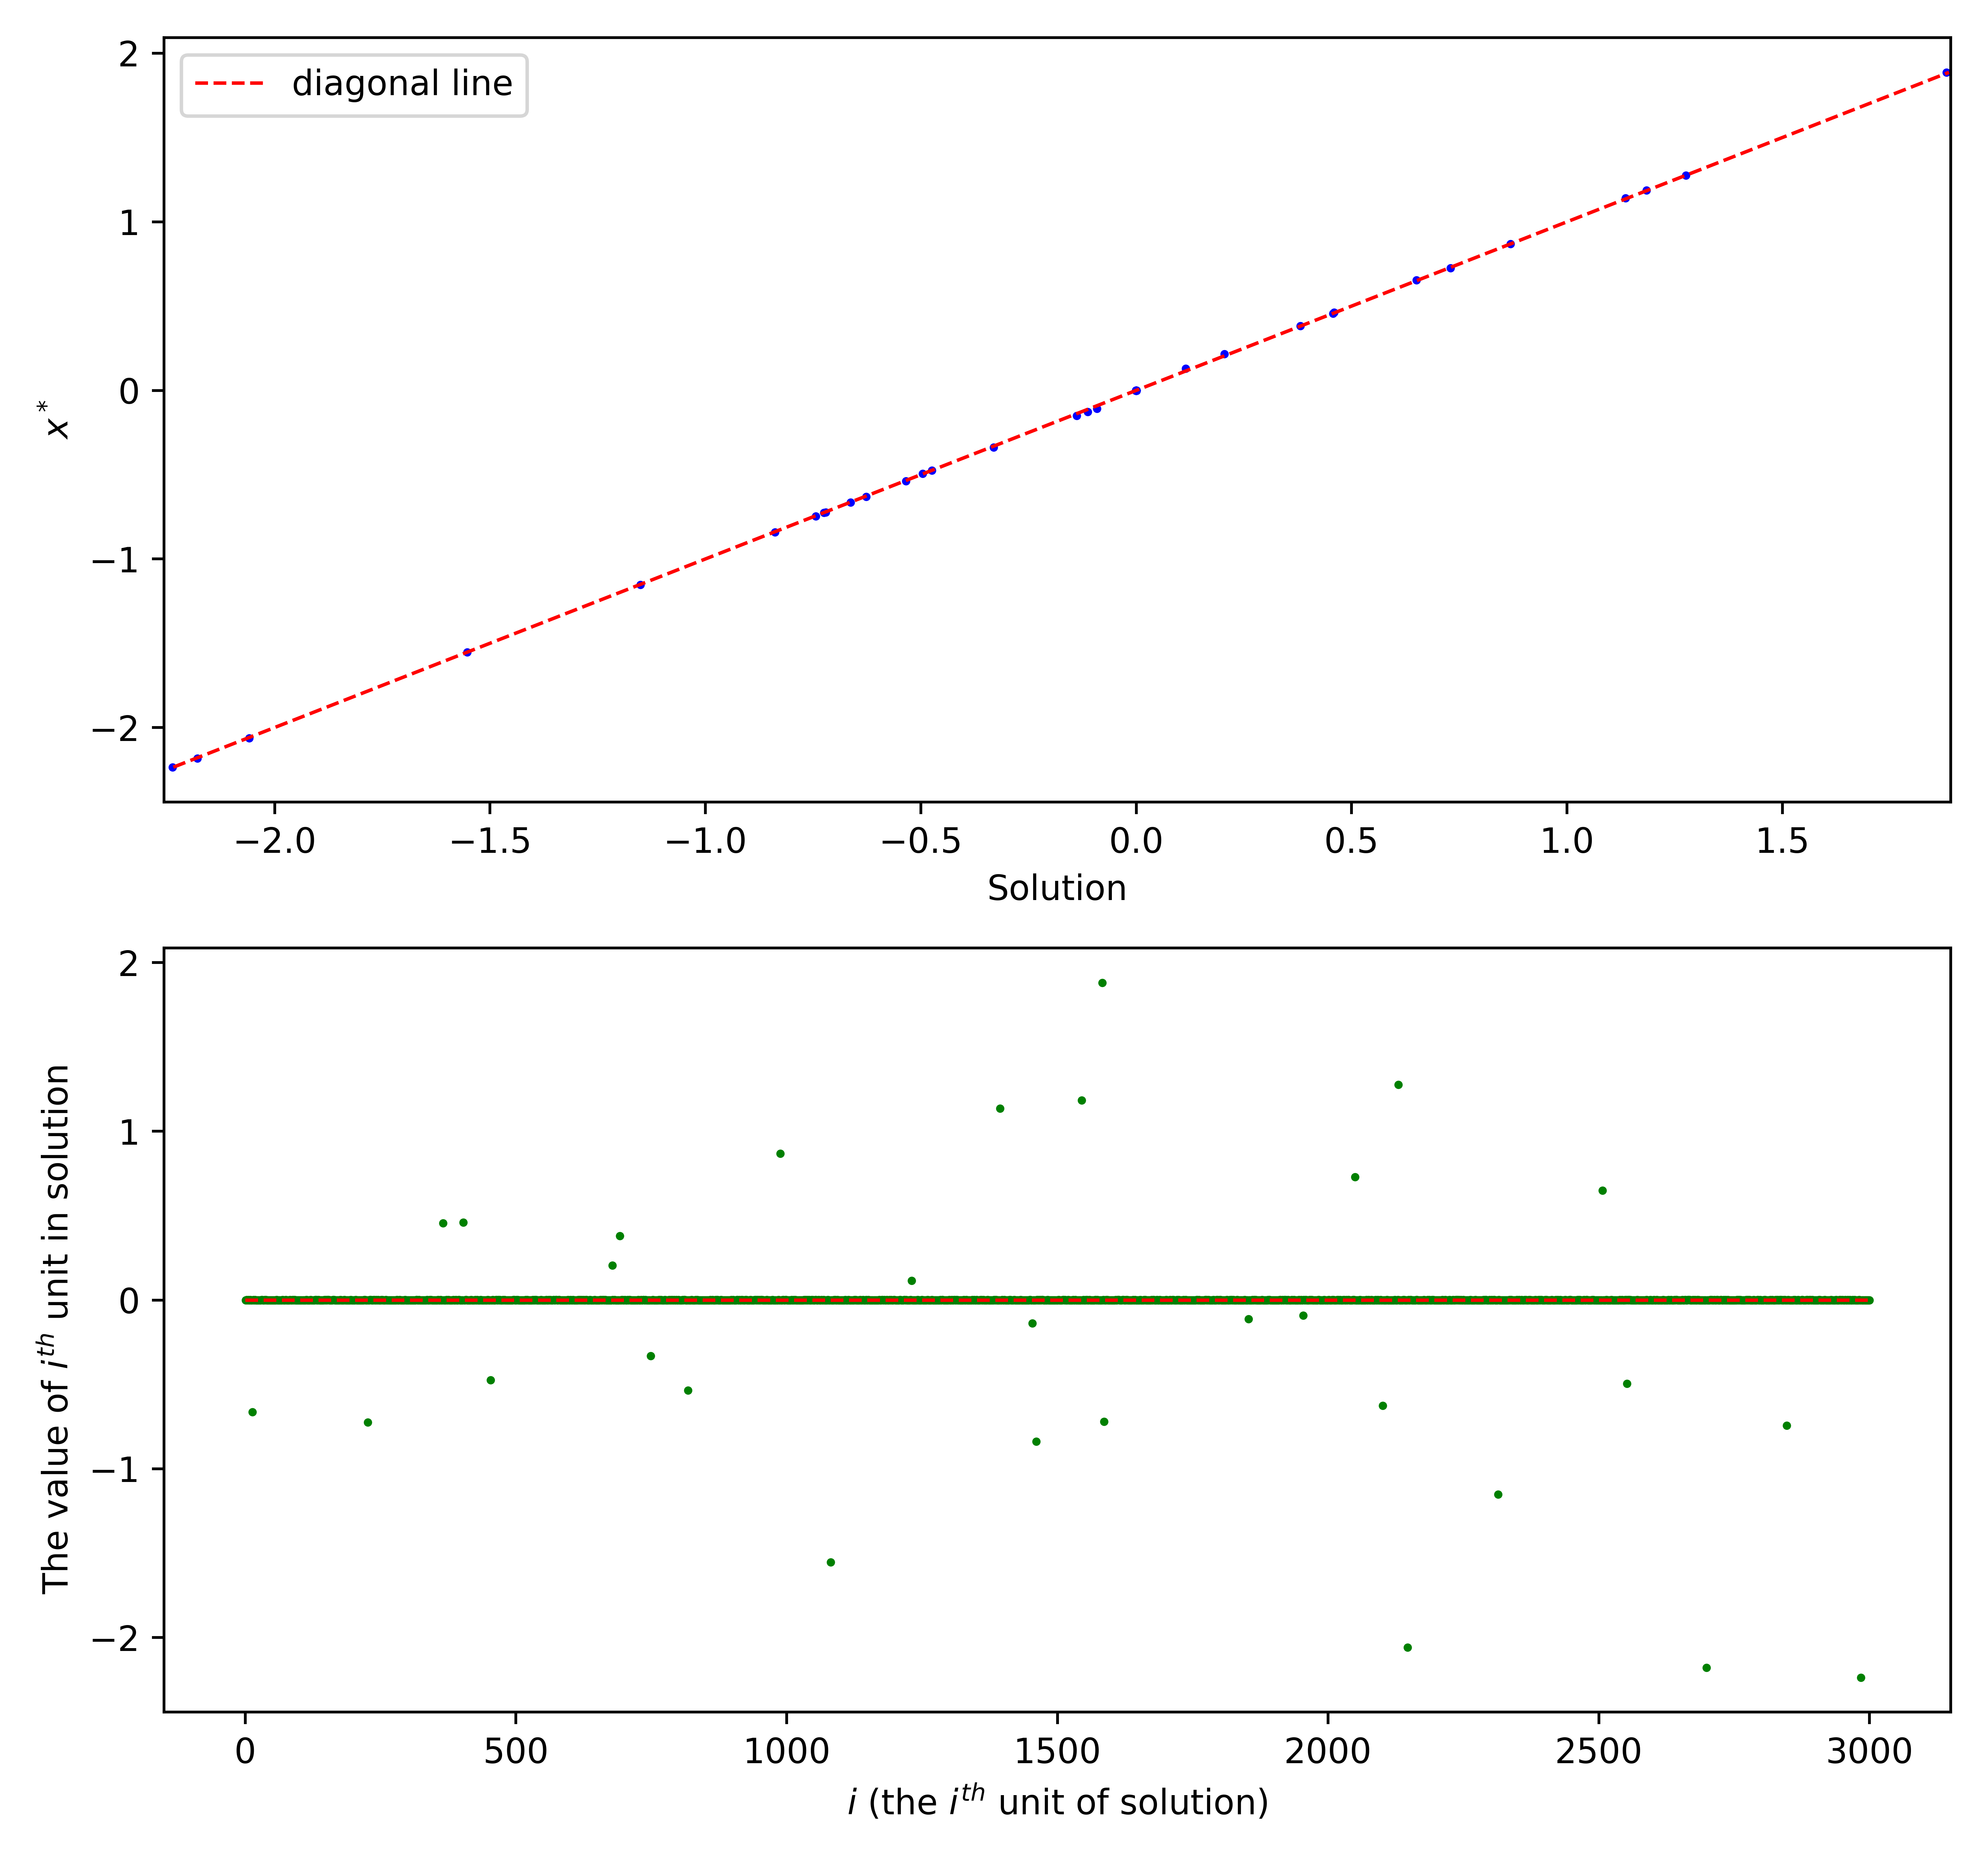
\includegraphics[width=0.3\linewidth]{compare_f3_UnknownL}}
			\caption{The comparison between solutions and $x^*$, and check the sparse of solutions}
			\label{compare_IGMunknownL}
		\end{figure}
		
		As we can see from Figure \ref{IGM2}, when we apply IGM with unknown $L$, the gradient of $f_1$ can converge in 52 times, the gradient of $f_2$ converges in 4835 times, and the gradient of $f_3$ converges in 1252 times. And we can see that there is a plateau period in the convergence process of the gradient of $f_2$ and the gradient of $f_3$.
		
		As we can see from Figure \ref{IGMf1_unknownL}, When using IGM with unknown $L$, $f_1$ is not a good model. This is because the solution is far away from $x^*$, which means the solution is not what we want. Besides, the solution is not sparse, there are small number of 0 in the solution's units actually. On the contrary, as we can see from Figure \ref{IGMf2_unknownL} and Figure \ref{IGMf3_unknownL}, when using IGM with unknown $L$, $f_2$ and $f_3$ are both good models. The solution is very close to $x^*$, because they are almost totally on the diagonal line. Besides, the solution is also sparse, there are just small number of units in the solution are not 0, but most units of them are 0, which means the solution is sparse.
		
	\end{enumerate}
	\item Summary
	
	Above all, we have applied AGM and IGM (with known $L$ and unknown $L$) method to solve $f_1$, $f_2$ and $f_3$ models respectively. The iteration times is concluded as Table \ref{performance3}.
	
	\begin{table}[htbp]
		\centering  % 显示位置为中间
		\caption{Performance of different methods on different models}  % 表格标题
		\label{performance3}  % 用于索引表格的标签
		%字母的个数对应列数,|代表分割线
		% l代表左对齐,c代表居中,r代表右对齐
		\begin{tabular}{|c|c|c|r|r|c|} 
			\hline  % 表格的横线
			& & & & &\\[-6pt]  %可以避免文字偏上来调整文字与上边界的距离
			Method&model&tolerance&iteration&time(s)& $\|x^k-x^*\|$\\
			\hline
			\multirow{3}{*}{AGM}
			& & & & &\\ [-6pt]  %可以避免文字偏上 
			&$f_1$&$10^{-4}$&62&0.978&4.775 \\
			& & & & &\\[-6pt]  %可以避免文字偏上 
			&$f_1$&$10^{-4}$&2023&115.113&0.085  \\
			\hline
			\multirow{3}{*}{IGM (know $L$)}
			& & & & &\\ [-6pt]  %可以避免文字偏上 
			&$f_1$&$10^{-4}$&52&0.406&5.392  \\
			& & & & &\\[-6pt]  %可以避免文字偏上 
			&$f_2$&$10^{-4}$&7276&417.809&0.086  \\ 
			\hline
			\multirow{5}{*}{IGM (not know $L$)}
			& & & & &\\ [-6pt]  %可以避免文字偏上 
			&$f_1$&$10^{-4}$&52&0.488&5.392  \\
			& & & & &\\[-6pt]  %可以避免文字偏上 
			&$f_2$&$10^{-4}$&4835&626.245&0.086  \\
			& & & & &\\[-6pt]  %可以避免文字偏上 
			&$f_3$&$10^{-4}$&1252&149.43&0.036  \\
			\hline
		\end{tabular}
	\end{table}
	As we can see from Table \ref{performance3}, model $f_3$ is the best in these tasks. When applied model $f_3$ with IGM and do not compute $L$ explicitly, the iteration times is 1252, which is smaller than model $f_2$. And the solution of model $f_3$ is the most close to $x^*$, as we can see the value  $\|x^k-x^*\|$ equals 0.036, which is very small.
\end{enumerate}
The python code to solve this problem is showed in subproblem(a) and subproblem(b) sections.
\end{homeworkProblem}
\end{document}

